%!TEX root=./LIVRO.tex
\hyphenation{tea-tro tea-tral so-cie-da-de}
\renewcommand{\fala}[1]{\noindent\quad\textsc{#1} ---}

\chapter[Introdução, \emph{por Larissa de Oliveira Neves}]{Introdução}
\hedramarkboth{Introdução}{Larissa de Oliveira Neves}

\begin{flushright}
\textsc{larissa de oliveira neves}
\end{flushright}

\textsc{A fortuna crítica} relacionada ao dramaturgo, contista, cronista e poeta
Artur Azevedo veio sofrendo uma transformação gradual nos últimos anos.
Batalhador incansável do teatro brasileiro, seu papel como “grande
animador”\footnote{ Expressão de Sábato Magaldi, em \textit{Panorama do teatro
brasileiro}, São Paulo, Global, 1997.} da cena nacional pouco foi contestado. No
entanto, mesmo as avaliações mais favoráveis ao seu talento cômico
mantiveram, por muito tempo, certo ar de condescendência; como se
apreciar o anedótico, o engraçado, o burlesco fosse invariavelmente
desabonador para uma pessoa culta. Felizmente, esse modo de pensar
sofreu uma gradativa reviravolta. Hoje, a obra de Artur Azevedo vem
sendo revisitada, dentro dos meios acadêmicos, a partir de leituras
menos preconceituosas, cujos resultados originaram e continuam a
originar importantes descobertas sobre nosso passado, nosso modo
de vida, nossa cultura --- cultura que, mesmo quando
realizada sob a forma de uma obra erudita, não deixa de conter traços
populares, característicos do que se passou a chamar de brasilidade.

Nesta edição, temos a honra de trazer a público cinco obras carregadas
de brasilidade. Essas peças foram escritas muito antes do surgimento
daquele famoso e polêmico grupo de escritores que surpreendeu o país
com suas obras literárias modernistas. As comédias deste volume
surgiram num momento em que vigorava um padrão literário que
privilegiava a gramática lusitana e os temas ditos elevados; um tempo em
que os intelectuais, nacionalistas a seu modo, ansiavam por ver o
Brasil se tornar um país tão civilizado, elegante e fino quanto os
países europeus, em especial a França. Não se imagine que Artur
Azevedo, por ter escrito essas peças, pensasse de modo diferente, ou
estivesse à frente de seu tempo. Não. Ele fazia parte daquele grupo de
intelectuais atuantes, cujos principais nomes foram Machado de Assis,
Olavo Bilac, Aluísio Azevedo (irmão de Artur) e Coelho Neto, entre
muitos outros. 

Artur Azevedo também se espelhava na França como fonte de uma cultura
mais refinada, e é aí que se constrói a sua figura paradoxal e
polêmica. Criticado pelos colegas fundadores da Academia Brasileira de
Letras por escrever comédias ligeiras, musicadas e populares, ele se
defendia sem proclamar uma igualdade de valor entre os gêneros
teatrais. Seu modo de pensar coadunava"-se com a visão dos demais
intelectuais de seu tempo, todos presos a padrões classicistas, que
repudiavam o teatro musicado. Tal concepção, porém, não o impedia de
realizar, na prática, o teatro para o qual seu talento o conduzia: um
teatro de diversão, em que a mistura de comicidade, de música e de uma
crítica bem"-humorada formam enredos divertidos e bem estruturados; em
que o vaivém das personagens, o ritmo acelerado e as peripécias
delineiam tramas bem urdidas e recheadas de surpresas.

Suas peças foram feitas para serem encenadas e apreciadas por uma
plateia eclética. O público que frequentava os teatros num tempo em que
não havia televisão, rádio ou cinema era composto por praticamente toda
a população do Rio de Janeiro, ricos e pobres (mais pobres do que
ricos, no caso do teatro musicado). Os ingressos mais baratos custavam
menos do que uma passagem de bonde: quase todos podiam ir ao teatro, ao
menos de vez em quando. Artur Azevedo escrevia peças pensando em
agradar toda a população, em fazer as pessoas se divertirem; para
tanto, seus textos são simples, escritos em linguagem brasileira, que
recria as características da fala coloquial da época. Ele utilizava os
próprios acontecimentos da vida real e os costumes da população para
criar as tramas; assim, a plateia identificava"-se imediatamente com as
personagens e as peripécias do enredo, e suas peças faziam grande
sucesso.

\section{A presente edição}

A presente edição contém cinco peças curtas de Artur Azevedo, sendo três
comédias de costumes em um ato: \textit{Amor por anexins}, \textit{A
pele do lobo }e \textit{O Oráculo}. Embora os estudos em torno da obra
do autor privilegiem as revistas de ano e as peças mais longas, são os
textos curtos os campeões em termos de encenação. Sem exigir um grande
número de atores ou aparatos de cena, as comédias em um ato têm sido
constantemente encenadas por grupos amadores e profissionais de todo o
país. Elas demonstram o quanto essa dramaturgia continua viva, atual,
com a capacidade de agradar espectadores mais de cem anos depois de sua
elaboração. Se a perenidade é um dos determinantes do valor de uma obra
de arte, não há dúvida de que esses textos sobreviveram ao seu tempo. 

Hoje em dia, é comum a apresentação de espetáculos teatrais curtos, de
meia hora ou quarenta minutos de duração, principalmente quando acontecem, por exemplo, em ambientes abertos, num espaço cênico
público. Assim, as comédias em um ato de Artur Azevedo têm ganhado
adaptações para a rua, sendo encenadas em praças e escolas. Se a ideia é
produzir um espetáculo mais longo, reúnem"-se dois ou três textos para
compor apresentações de uma a duas horas de duração. Quando foram
escritas, porém, sua função era outra: no século \textsc{xix}, as pecinhas
cômicas tinham espaço garantido como complemento de tragédias, dramas
ou melodramas longuíssimos. Os espetáculos se estendiam por três a
quatro horas, e os textos curtos funcionavam como momentos de
relaxamento entre os atos ou no encerramento da noite. 

Além disso, as peças curtas ganham um novo sabor nas páginas de um
livro, porque, diferentemente de textos cuja teatralidade supera a
literariedade, como é o caso das revistas de ano, é possível desfrutar
plena e prazerosamente dos enredos através de uma leitura solitária.
Não é à toa que tais textos, ainda no século \textsc{xix}, eram publicados em
jornais, revistas, livros ou brochuras, após as encenações.\footnote{
Para informações mais detalhadas, ver Orna Messer Levin, “Teatro de papel -- certa dramaturgia de Artur Azevedo”, em Orna M. Levin e Larissa O. Neves, \textit{Teatro,
literatura e imprensa na virada do século}, revista \textit{Remate de
Males }28.1, Campinas, IEL, jan.--jun.
2008.}

Junto às três comédias em um ato, este livro inclui duas outras peças,
cujo tema é o carnaval. \textit{Como eu me diverti!}, curtíssima, foi
publicada no livro \textit{Contos fora de moda}, de 1894. Classificada
pelo autor como conto"-comédia, a peça demonstra o quanto a teatralidade
está presente em toda a obra literária de Artur Azevedo, seja sob a
forma de conto, crônica ou poesia.\footnote{ Sobre a teatralidade na
poesia de Artur Azevedo, ver Pedro Marques, \textit{``Artur
Azevedo e a arte do soneto dramático''}, \textit{idem.}} Isso se comprova,
também, com a peça \textit{O Oráculo}, já que ela é nada mais nada
menos do que a transposição para a cena do conto \textit{Sabina},
escrito em 1894. Já \textit{O Cordão}, embora apenas ligeiramente mais
extensa que as outras comédias, é uma peça de complexidade maior: uma
burleta, gênero que engloba as melhores obras do autor, como \textit{A
Capital Federal} e \textit{O Mambembe}. \textit{Como eu me diverti!} e
\textit{O Cordão} são interessantíssimas por delinearem a ambiguidade
intelectual do escritor mediante uma crítica bonachona relacionada ao
carnaval. 

\section{Três pequenas comédias}

\paragraph{Amor por anexins}
\textit{Amor por anexins} é a primeira peça de Artur Azevedo, se não
levarmos em consideração uma pecinha escrita aos nove anos de idade,
cujo texto está perdido.\footnote{ Raimundo Magalhães Jr.,
\textit{Artur Azevedo e sua época}, São Paulo, Livros
Irradiantes, 1971.} Tinha ele apenas quinze anos e ainda residia
em São Luís do Maranhão, sua cidade natal, quando empreendeu a primeira
incursão séria na arte dramática (séria no sentido de que elaborou
a comédia para ir à cena, representada por duas atrizes, as irmãs
Riosa). Apenas três anos depois, em 1873, ele se mudaria para o Rio de
Janeiro, para onde se dirigiam praticamente todos os jovens com
aspirações literárias no século \textsc{xix}. Sem esquecer o Maranhão, o
comediógrafo tornou"-se um grande satirista dos costumes da capital,
cenário de quase todas as suas peças. \textit{Amor por anexins}, após
ser apresentada pelas irmãs Riosa “em quase todo o Brasil e até em
Portugal”,\footnote{ Citação de Artur Azevedo, \textit{apud } Antonio Martins Araújo, \textit{Teatro de Artur Azevedo}, Rio de Janeiro, Funarte, 2002, v. 4, p. 59.} ganhou sua primeira edição em livro no
ano de 1879, e continuou a ser encenada como entreato de peças maiores
nas décadas seguintes. 

O sucesso dessa pecinha, cujo enredo se baseia no tantas vezes explorado
tema do enamorado velho e endinheirado que persiste na conquista
amorosa de uma jovem, reside no modo como o autor caracterizou o
solteirão Isaías; o cacoete da personagem, que fala o tempo todo por
meio de anexins, torna o texto não só engraçado como extremamente
original. A habilidade com que o escritor soube enfileirar os
provérbios, posicionando"-os uns após os outros de modo a transmitir de
maneira verossímil as ideias da personagem, demonstra o quanto ele,
ainda tão jovem, possuía pleno domínio do uso da língua, além de um forte
talento para a dramaturgia popular. 

A ideia da peça pode ter surgido da leitura da obra \textit{Metáforas ou
feira dos anexins}, do escritor português Francisco Manuel de Mello.
Apesar de a primeira edição desse livro, póstuma, datar de 1875, existe
a possibilidade de o menino Artur ter tido acesso à obra por intermédio
do pai, o cônsul português David Gonçalves de Azevedo, tendo em vista
que em 1840 já se sabia de sua existência e de sua suposta utilidade,
conforme atesta a seguinte citação:

\begin{hedraquote} 
\mbox{}[\ldots{}] livro curioso, em que estão lançadas metodicamente as metáforas e
locuções populares da língua portuguesa, e que seria quase um manual
para os escritores dramáticos, principalmente do gênero cômico, que
quisessem fazer falar as suas personagens com frase conveniente, e com
as graças e toque próprio da nossa língua portuguesa e do verdadeiro
estilo dramático.\footnote{ Herculano, \textit{apud }Francisco
Manuel Mello, \textit{Metáforas ou a feira dos anexins}, www.dominiopublico.gov.br/download/texto/ub000005.pdf
(consultado em 08/01/2009.}
\end{hedraquote} 

Mesmo que Artur Azevedo tenha lido a obra e, inclusive, o conselho
transcrito acima, tendo decidido segui"-lo (fato que não passa de mera suposição), isso não diminui a importância de sua proeza, porque o
livro \textit{Feira dos anexins}, afora os anexins, pouco, ou quase
nada, tem de semelhante com a comédia \textit{Amor por anexins}. O
primeiro consiste em duas séries de contos dialogados --- nas quais
se discute o valor e a relevância de anexins de todos os tipos e, para
tanto, os contendores utilizam"-se dos próprios provérbios como recursos
de arrazoamento --- e numa série de anedotas temáticas, também
narradas por meio de trocadilhos, metáforas e ditados populares. 

Já em \textit{Amor por anexins}, o impertinente e tagarela
Isaías invade a casa de sua amada, a viuvinha Inês, disposto a não sair
de lá antes de convencê"-la a se casar com ele. A peça nada tem de
romantismo exacerbado: as duas personagens são movidas por interesses
menos nobres do que o amor sincero (este virá depois). Sem arroubos de
paixão, Isaías, cansado da vida de solteiro, simplesmente decidiu se
casar e escolheu Inês por ela ser boa dona de casa e honesta. A jovem
senhora, por seu turno, também não quer permanecer viúva, mas rejeita
Isaías, num primeiro momento, porque já tem um noivo jovem e bonito ---
que também não ama, haja vista a rapidez com que se consola após
receber a carta em que o rapaz rompe o compromisso.  Desdenha,
portanto, a oferta do velho, feio e maçante solteirão enquanto supõe
que tem um partido melhor, mas logo muda de ideia, com medo de
permanecer viúva. A despeito de suas imperfeições, as personagens são
carismáticas e a conversa que entretêm conduz, invariavelmente, ao
riso. 

Além do diálogo fluido e engraçado, a pequena comédia também se
enriquece com os versos, escritos para serem cantados pelas personagens
em momentos especialmente escolhidos. Grande mestre do teatro musicado,
cujos gêneros (a revista, a opereta e a burleta) mesclam momentos
dialogados com canções temáticas, nas quais as personagens revelam seus
sentimentos ao público ou umas às outras, Artur Azevedo mostra, em sua
primeira peça, que o talento para compor versos simples, facilmente
musicáveis, sempre fez parte de sua índole artística. A simplicidade
das estrofes de \textit{Amor por anexins} permitiu que fossem criadas
diferentes partituras para as mesmas no decorrer dos anos, sendo que a
primeira, de Leocádio Raiol, está perdida. 

Esse texto de estreia, portanto, contém inúmeros indícios do caminho a
ser percorrido pelo seu autor: a comicidade, a simplicidade, a crítica
zombeteira, o trabalho com a linguagem popular e os números musicados.

\paragraph{A pele do lobo}
Artur Azevedo escreveu \textit{A pele do lobo} em 1875, mas a peça foi
encenada pela primeira vez em 1877, como complemento da opereta
\textit{Abel, Helena}. Esta última é uma adaptação, do próprio Artur,
de \textit{La belle Helène }(de Offenbach), texto francês de gênero
musicado que fazia bastante sucesso à época. Para a festa em homenagem
ao autor, realizada no dia 10 de abril, a companhia do teatro Fênix
Dramática exibiu a inédita comédia em um ato \textit{A pele do lobo},
junto com a opereta, que já estava em cartaz.

Os textos curtos, em geral, não tinham grande repercussão na imprensa,
porque eram considerados apenas adendos do espetáculo principal.
\textit{A pele do lobo }foi publicada na \textit{Revista do Rio de
Janeiro}, periódico para o qual Artur Azevedo escrevia crônicas e
poemas, no mesmo mês em que estreou no teatro. O texto, uma típica
comédia de costumes, retrata, ao mesmo tempo em que critica, uma das
esferas do meio social da época.

Em \textit{A pele do lobo} a crítica social surge diretamente, o que não
faz essa comédia ser menos engraçada para o leitor/\,espectador de hoje.
Pelo contrário, ela demonstra que, se algumas coisas mudaram, outras
continuam sendo as mesmas. Se escarrar em público é hoje uma prática
inconcebível, uma tremenda falta de educação --- fato que torna ainda
mais cômica a cena em que Jerônimo suja a casa de Cardoso porque “a
casa da autoridade é uma repartição pública” ---, a falta de
reconhecimento do trabalho público, de um lado, \mbox{e o} interesse pessoal
por trás daqueles que “metem"-se a servir o país”, de outro, continuam
sendo atuais.

O enredo, por si só, é bastante divertido: a personagem principal, o
subdelegado Cardoso, tenta sair com sua esposa, Amália, para ir a uma
cerimônia de batizado, na qual serão os padrinhos, mas são
interrompidos continuamente pelas pessoas que chegam para “dar parte”
de pequenos crimes ou irregularidades. O casal, cada vez mais nervoso,
só consegue sair após três horas de contrariedades, com direito a
correria e confusão.

Na segunda metade do século \textsc{xix}, homens notáveis na sociedade, ao serem
nomeados pelo poder imperial, por meio dos presidentes das províncias,
exerciam, gratuitamente, as funções de delegado e de subdelegado. Cabia
a eles zelar pela manutenção da ordem pública, bem como desempenhar
funções administrativas e, após 1871, preparar inquéritos policiais. A
indicação envolvia jogos de interesse e politicagem. A rotatividade de
delegados e subdelegados era intensa: poucos se mantinham por muito
tempo nos cargos. 

\begin{hedraquote} 
O serviço não"-remunerado muitas vezes não valia as compensações laterais
que o uso do fitão, o símbolo por excelência da autoridade policial,
proporcionavam. Assim, as queixas e pedidos de desligamento eram
igualmente copiosos. E, apesar da obrigatoriedade do aceite, muitas
declinações eram acolhidas pelo governo.\footnote{ André Rosemberg,
\textit{Polícia, policial e policiamento na província de São Paulo, no
final do Império: a instituição, prática cotidiana e cultura} (tese de
doutorado), São Paulo, USP, 2008, p. 44.}  
\end{hedraquote} 

Como se vê, em \textit{A pele do lobo} Artur Azevedo fez uma justa e
cômica crítica aos costumes policiais do Brasil imperial. Cardoso
solicita uma subdelegacia com vistas a uma futura promoção; trabalha
noite e dia atendendo as “partes”, a ponto de levantar"-se de madrugada
e deixar de sair para um batizado a fim de cumprir o dever; ainda
assim, publicam"-se “descomposturas” sobre ele no jornal. Tanta
dedicação de nada lhe adianta, já que perde a promoção, ao mesmo tempo
em que é demitido da subdelegacia.

A comicidade fica por conta da ingenuidade do caipira Apolinário; da
malandragem de Jerônimo; das saídas falsas do casal, a cada momento
impedido por algo ou alguém; e pelo chavão, repetido constantemente por
Cardoso:

\begin{hedraquote}
\fala{Cardoso} E metam"-se!

\fala{Amélia} Hein?

\fala{Cardoso} E metam"-se a servir o país!
\end{hedraquote}

\paragraph{O Oráculo}
O enredo da comédia \textit{O Oráculo} partiu de um conto próprio,
chamado \textit{Sabina} e publicado no jornal \textit{O País}, em 25 de
março de 1894. Em 1903, Eduardo Vitorino, empresário e dramaturgo
português que trabalhou durante muitos anos no Brasil, pediu a Artur
Azevedo uma peça em um ato para compor o programa de um espetáculo. O
comediógrafo, lembrando"-se do conto, por si só bastante teatral,
escreveu \textit{O Oráculo}, cuja personagem central, Helena, foi
criada especialmente para Georgina Pinto, primeira atriz da companhia.
A atriz, no entanto, faleceu de febre amarela antes da encenação, e
\textit{O Oráculo} ficou à espera de uma nova oportunidade. Esta surgiu
com o espetáculo em benefício do autor, ocorrido no dia 2 de abril de
1907, durante as representações de \textit{O dote}, comédia de Azevedo
que fez imenso sucesso naquele ano. Desta vez, o papel principal coube
à atriz brasileira Guilhermina Rocha. O crítico do jornal \textit{O
País} escreveu, à época, o seguinte comentário sobre o texto:

\begin{hedraquote} 
Simples, de urdidura delicada, facilmente apreensível, \textit{O Oráculo} tem 
as qualidades conhecidas da arte dramática de Artur Azevedo, cuja
penetrante observação, fluência e espontaneidade do diálogo e
propriedade de cena fizeram, há muito, dele o nosso melhor
comediógrafo.\footnote{ “Artes e Artistas. Primeiras Representações”,
em \textit{O País}, 04/04/1907.}
\end{hedraquote} 

O comentário descreve adequadamente as qualidades da peça. O enredo,
simples e curto, não permite um aprofundamento emotivo sobre o tema;
como nas outras comédias curtas do autor, a simplicidade fornece o
ritmo acelerado ao desenvolvimento da fábula, o que não significa que
esta peque por falta de continuidade ou verossimilhança: pelo
contrário, trata"-se de um texto de urdidura bastante coesa. 

A comédia é, em verdade, uma bela transposição para a linguagem cênica
de \textit{Sabina}, conto que narra a história do romance entre o
solteiro Figueiredo e a viúva Sabina (Nélson e Helena na comédia); no
começo do namoro, ela recusa o pedido de casamento, pois acredita que
oficializar a relação esfriaria rapidamente o amor de Figueiredo; após
dois anos (três na peça), no entanto, ele se sente cansado da viúva,
independentemente de ter permanecido solteiro e, querendo pôr fim ao
namoro, pede conselhos ao velho solteirão Matos (Frederico, na comédia),
considerado um oráculo em questões de amor. O amigo aconselha
Figueiredo a acusar Sabina de algum “mau passo”, mesmo sabendo da
honestidade de sua amante, abandonando"-a em seguida sem maiores
explicações. Sabina, porém, usa de esperteza para “segurar” o namorado
e casar"-se com ele: ao receber a acusação, aceita e confessa a falta,
embora não o tenha de fato traído; ele, louco de ciúme, pede"-a em
casamento.

Na peça, além da inclusão da personagem José, empregado de Nélson, de
grande importância para a crítica social e para a comicidade, a única
diferença no enredo consiste no fato de que Helena, escondida, ouve a
conversa entre seu amante e Frederico. Sabendo antecipadamente o
artifício a ser utilizado por Nélson para afastar"-se dela, pode, com
argúcia, inventar um erro no passado para prendê"-lo pelo ciúme. Assim,
a fábula ganha consistência no texto dramático, em que as ações das
personagens se justificam --- podemos afirmar, inclusive, que a comédia é
superior ao conto. 

As informações fornecidas pelo narrador, no conto, são permeadas com
naturalidade na peça entre as falas das personagens, sem dar impressão
de artificialidade. Dois monólogos explicam ao leitor/\,espectador a
situação vivida pelo casal: logo na primeira cena, José, “refestelado
na poltrona com um espanador na mão, a saborear um charuto”, conversa
com o público; vangloria"-se de sua vida ociosa como empregado de
Nélson, já que o patrão vive na casa de sua amante, a “viúva de
Laranjeiras”. O monólogo é espirituoso, espontâneo e engraçado,
características que o impedem de se assemelhar a uma mera muleta
narrativa. Logo depois, Helena entra à procura de Nélson; ela está
nervosa com o descaso demonstrado pelo namorado nos últimos tempos;
sozinha, reflete em voz alta:

\begin{hedraquote} 
\fala{Helena} Não há que ver: está farto de mim! Desfez o encanto! Tudo
acabou. Já o esperava: há muitos meses noto a mudança do seu entusiasmo
de outrora. Melhor seria que nos houvéssemos casado. E dizer que fui eu
que não quis! Dei"-me tão mal com o casamento, que não me sorriu
experimentá"-lo de novo. Era bem independente para não me importar com o
que dissessem. (\textit{Senta"-se e ergue"-se logo em seguida, cada vez
mais agitada}.) Mas não! É impossível que Nélson seja ingrato. Há três
anos pertenço"-lhe, e nunca tive outro amor, nunca pensei em outro
homem.
\end{hedraquote} 

O curto monólogo informa sobre a situação do casal --- o passado, a
honestidade e hesitação de Helena, o desinteresse de Nélson --- sem se
caracterizar como um enfadonho relato. A angústia da personagem, que
fala a si mesma sobre os próprios sentimentos, justifica plenamente o
recurso; não há quebra no ritmo, no andamento da trama que se inicia;
por fim, a transposição de fatos narrados no conto em terceira pessoa
para a linguagem dramática ocorre sem qualquer artificialismo.
\textit{O Oráculo} mantém toda a graciosidade da narrativa, chegando
até a superá"-la, não só porque no texto dramático há a explicação sobre
os motivos que levam Helena a urdir seu estratagema, mas também porque
se nota uma crítica social espontânea e cômica, realizada por meio dos
comentários ferinos e recheados de humor proferidos por José.

A personalidade deste tipo cômico baseia"-se na tradição da comédia.
Desde a Antiguidade, até hoje, o empregado da casa é uma personagem
frequente das comédias, capaz de facilitar a representação dos costumes
e geralmente responsável por vários episódios engraçados do enredo. Não
raro, tal personagem centraliza as ações, conduz o enredo e manipula a
vida das demais personagens (devemos lembrar que esse tipo,
desenvolvido na comédia tradicional francesa, surgiu a partir das
personagens da antiga comédia italiana, a \textit{Commedia dell’Arte},
e pode ser encontrado também em peças clássicas de outros países
europeus). Em \textit{O Oráculo}, a influência da tradição surge de
maneira bem explícita, porque José se parece com os criados originais
da \textit{Commedia dell’Arte} (os chamados “zanni”, que compunham o
grupo de personagens mais populares da \textit{Commedia}, o que explica
sua enorme influência na comédia posterior): ele lembra o esperto e
bufão Arlequim, sempre no centro das intrigas.

Empregado de Nélson, José vive refestelado na poltrona, sem nada fazer,
a fumar os charutos de seu amo; português, quem o trouxe ao Brasil foi
o comendador Frederico, o “oráculo do amor”, mas este não aguentou
conviver com um empregado tão ladino. Numa passagem da peça, Frederico
compara seu antigo criado com personagens clássicas do teatro francês,
revelando abertamente ao leitor/\,espectador o diálogo de Artur Azevedo
com a tradição francesa, que ele conhecia tão bem:

\begin{hedraquote} 
\fala{Frederico} Convenci"-me de que tinhas espírito demais para um simples
criado. Os Scapins\footnote{ Scapin, criado na comédia \textit{Les
fourberies de Scapin} (1671), de Molière.}  e os Frontins\footnote{
Frontin, criado na comédia \textit{Marton et Frontin} (1804), de
Jean"-Baptiste Dubois.} só me agradam na \textit{Comédie} ou no Odeon.
Fora dali acho"-os detestáveis. Entretanto, ao saíres de minha casa,
poderias aspirar a coisa melhor\ldots{} Por que não te arranjaste no
comércio?

\fala{José} Não sou ambicioso\ldots{} Agrada"-me esta situação\ldots{} considero"-me
colocado melhor que o meu amo.
\end{hedraquote} 

Satisfeito com sua posição de criado de um homem solteiro, José não
ambiciona qualquer outro trabalho, em que, certamente, não poderia
passar o dia descansando, a passear pela cidade, a comer e beber do
melhor e a fumar bons charutos. A comicidade do tipo apresenta"-se não
só em sua personalidade alegre e prazenteira, mas também em suas
tiradas irônicas, relativas ao namoro do patrão e ao seu escritório de
advocacia sem clientes: 

\begin{hedraquote} 
\fala{José} O amo nunca está em casa, e eu faço de conta que tudo é nosso.
Permita Deus que tão cedo não acabem os seus amores com a tal viúva das
Laranjeiras.

\fala{Helena} Então algum cliente?

\fala{José} Seria um fenômeno, mas\ldots{} quem sabe? Tudo acontece. Não fizeram a
avenida?\footnote{ Referência à avenida Central (hoje Rio Branco),
recém construída durante as famosas reformas encetadas pelo prefeito
Pereira Passos na virada do século \textsc{xix}--\textsc{xx}. As reformas modificaram
profundamente o centro do Rio de Janeiro.}

\fala{José} Logo vi que Vossa Excelência vinha para ser consultado. Para
consultar ainda está para ser o primeiro que aqui venha.
\end{hedraquote} 

A última fala lhe pertence e fecha com graciosidade a comédia; ao saber
do casamento do patrão, cuja consequência seria uma mulher a cuidar da
casa onde ele trabalha, José se dirige à plateia:

\begin{hedraquote} 
\fala{José} (\textit{À parte}) Ele casa"-se!\ldots{} Adeus, beatitude!\ldots{}
Sua boa vida está com os dias contados\ldots{} 
\end{hedraquote} 

Nessa curta peça de costumes, Artur Azevedo demonstra toda a sua
habilidade em criar um enredo engraçado, que prende a atenção do
leitor/\,espectador, e ainda reelabora elementos da tradição literária.
Além disso, critica a ociosidade de maneira extremamente divertida:
Nélson, por ser rico, pode passar as horas a namorar, sem se preocupar
com a falta de clientes e sem ser criticado por causa disso pelas
pessoas de seu meio social; já José, o empregado, aproveita a boa vida
do patrão para, ele próprio, viver entre charutos e passeios. Como
pobre que é, no entanto, precisa fingir que trabalha, e é considerado
um malandro pelas pessoas da alta sociedade. A hipocrisia do pensamento
vigente em nossa sociedade até os dias de hoje apresenta"-se clara no
texto teatral: os ricos podem viver entre os prazeres da ociosidade; já
os pobres, se não trabalham, são considerados vagabundos.

A crítica, nesta comediazinha bem estruturada, surge nas entrelinhas,
entre as ações e diálogos, de maneira natural; a ironia presente nas
falas de José propicia o riso, retrata a sociedade e demonstra o poder
de crítica presente na comicidade. O talento do autor nesse sentido
pode ser apreciado tanto em suas melhores comédias de costumes quanto
nas peças musicadas. Grande observador de pessoas e hábitos, arguto
para tirar proveito máximo de aspectos da sociedade capazes de levar o
espectador ao riso, ele soube transpor para a linguagem cênica o Brasil
em que viveu. 

\section{Duas comédias sobre o carnaval}

\paragraph{O carnaval}

O carnaval, a maior festa popular brasileira, sempre uniu o povo nos
dias de folia. No entanto, no Rio de Janeiro do final do século \textsc{xix},
que ansiava por ser a capital de um país moderno e civilizado, havia um
grande preconceito, por parte da elite intelectual e econômica,
relativo ao carnaval brincado pela população mais pobre. Os
intelectuais consideravam os desfiles e bailes organizados pelos ricos
superiores à alegre desordem vista entre a população em geral. No
desejo de “civilizar” a nação brasileira incluía"-se o intuito de
moderar a “balbúrdia” presente na festa dos pobres. O carnaval ideal,
para os escritores, seria aquele comandado pelas sociedades
carnavalescas ricas. Os Tenentes do Diabo, Democráticos e Fenianos eram
os três grupos mais famosos, compostos por pessoas de poder aquisitivo
alto, que pagavam mensalidades caras durante o ano para desfilar com
fantasias e em carros luxuosos durante o carnaval.

Quem não tinha condições, porém, de participar dos desfiles das
sociedades, ou dos bailes bem"-comportados frequentados pelas famílias
ilustres, não deixava de se divertir: os cordões, ou zé"-pereiras,
compostos pelas pessoas pobres ansiosas pela diversão dos dias de
carnaval, pululavam atrás dos desfiles das ricas sociedades. A situação
nos lembra, hoje, os caros abadás, obrigatórios para os acompanhantes
oficiais dos trios elétricos, e os “pipocas”, que seguem os trios sem
pagar nada. 

A maioria dos literatos, fazendo"-se de porta"-voz das damas e senhores da
alta sociedade, criticava a dança gingada, a música de origem africana,
a bagunça, as brigas, a bebedeira dos cordões, em oposição aos belos
carros alegóricos das sociedades. A mistura das diferentes classes
sociais durante o carnaval expunha a todos a pobreza e o modo de vida
das pessoas marginalizadas. Nesses dias, tornava"-se evidente a todos,
em desfiles nas ruas centrais da capital, as expressões culturais
(música, dança, luta da capoeira) que a intelectualidade procurava
“regenerar”, ou seja, suprimir.\footnote{ Para maiores informações, ver Leonardo Affonso M. Pereira, \textit{Carnaval
das letras}, Rio de Janeiro, Secretaria Municipal de Cultura, 1994, e Nicolau Sevcenko, \textit{Literatura como missão:
tensões sociais e criação cultural na Primeira República}, São Paulo, Companhia das Letras, 2003.}

Artur Azevedo, apesar de concordar em parte com esse posicionamento,
diferenciava"-se dos demais escritores por escrever para um público
popular, para aquelas mesmas pessoas cujos hábitos eram tão criticados.
Ao aproximar"-se do povo através do teatro ligeiro, a sua posição
frente aos costumes considerados “bárbaros” adquire ares extremamente
simpáticos. Sua afinidade com a cultura popular brasileira apresenta"-se
na empatia com que caracterizou o desacordado folião de \textit{Como eu
me diverti!} e o povo da lira, isto é, os componentes do grupo “Foliões
do Itapiru”, da burleta \textit{O Cordão}.

\paragraph{Como eu me diverti!}

O conto"-comédia \textit{Como eu me diverti!}, pela extensão, é o que
hoje se denomina esquete teatral. Se encenado junto com outras peças
curtas de Artur Azevedo, ou de outros autores, pode originar um
espetáculo dinâmico e interessante.\footnote{ Em 2008, o projeto
Clássicos do Teatro, da cidade do Rio de Janeiro, apresentou a leitura
dramatizada de quatro peças de Artur Azevedo: \textit{Amor por
anexins}, \textit{Entre o vermute e a sopa}, \textit{Uma noite em claro
}e \textit{Como eu me diverti!}, realizada pelo grupo Teatro de Roda.}
Tudo indica, porém, que o autor escreveu o texto para ser publicado, e
não encenado, não obstante sua teatralidade --- presente, aliás, em
diversos de seus contos (dialogados ou narrados).

Além de ser engraçada e ter um final inusitado, essa pecinha revela a
ambiguidade do escritor em relação ao carnaval. Um rapaz, após uma
noite de diversão durante o carnaval, retorna, bêbado e passando mal, à
pensão onde mora. Em virtude de seus excessos, acaba perdendo a noiva e
o emprego, porque seu chefe e o padrinho da moça (o médico que, por
coincidência do destino, vem examiná"-lo a pedido da dona da pensão)
descobrem o deslize. O jovem em torno do qual o esquete se desenvolve
tem apenas uma fala, aquela que fecha o enredo. Essa frase --- por,
ao mesmo tempo, encerrar e intitular a obra --- propicia um sorriso
no rosto do leitor/\,espectador e transmite, ainda que nas entrelinhas, a
simpatia do autor pela festa popular. 

A crítica severa dos dois senhores moralistas que, com tanta indignação,
repreendem as loucuras cometidas pelo jovem nos dias de carnaval perde
a força e torna"-se, apenas, cômica, quando o jovem, ao final, entreabre
os olhos, sorri e “exclama com voz rouca e sumida”, sem saber das
dificuldades que o aguardam quando a ressaca passar: “Como eu me
diverti!”. Não há como não simpatizarmos com o protagonista, tão
defendido por Dona Maria, a dona da pensão, até porque são poucos os
brasileiros que nunca cometeram suas pequenas ou grandes loucuras
durante o carnaval. E, por transmitir essa simpatia, o mais provável é
que o escritor também a sentisse.

\paragraph{O Cordão}
A hipótese acima ganha força quando analisamos a burleta \textit{O
Cordão}, encenada durante o carnaval de 1908. As burletas são peças de
um gênero que engloba, num mesmo texto, as diferentes manifestações do
teatro musicado: enredo cômico de temática brasileira, permeado por
números musicais, com muitas personagens e variadas mudanças de
cenário. \textit{O Cordão}, apesar de ser a burleta mais curta e uma
das menos conhecidas de Artur Azevedo, chama a atenção por diversos
motivos: a inclusão, em primeiro plano, de personagens oriundas da
periferia urbana do Rio de Janeiro; a linguagem repleta de gírias e
oralidades, que caracteriza cada personagem; a ambiguidade na abordagem
da temática do carnaval, que, de modo mais saliente que em \textit{Como
eu me diverti!}, demonstra o perfil intelectual de seu autor.

O enredo dessa burleta teve origem em um episódio da revista de ano
\textit{Comeu!}, de 1902. O segundo quadro de \textit{O Cordão}
consiste na transposição quase idêntica do quarto quadro de
\textit{Comeu!}, publicado no jornal \textit{O País}, em 28 de julho de
1904. Artur Azevedo acrescentou alguns episódios, de modo a formar um
enredo coeso: Remígio, um praça reformado do exército, participa
assiduamente dos cordões nos dias de folia; suas filhas, Florinda e
Rosa, educadas por um padrinho, são avessas à festa. Os namorados das
moças, Alfredo e Gastão, funcionários de repartição, desejam afastá"-las
desse ambiente --- considerado, por eles, maléfico à sua “pureza”. O
namoro serve de pretexto para a exposição dos costumes e para a crítica
social, que decorre da diferença nos modos de pensar, agir e falar
entre as personagens instruídas (os namorados e o chefe da repartição
na qual trabalham, chamado de Conselheiro) e as personagens da
periferia (os participantes costumeiros do cordão \textit{Foliões do
Itapiru}, do qual faz parte Remígio).

A partir da oposição existente entre as personagens da burleta, é
possível dividi"-las em dois grupos. No primeiro incluem"-se as
personagens formalmente educadas, com emprego fixo: os dois rapazes,
Gastão e Alfredo; as moças, Florinda e Rosa (educadas por um padrinho
General), e o Conselheiro. Do “grupo do Cordão” fazem parte os
membros assíduos do “Cordão Carnavalesco Foliões do Itapiru”:
Remígio e seus companheiros de folia, pobres e analfabetos. À primeira
vista, sobressai no texto a crítica aos costumes do “grupo do Cordão”,
expressa pelas personagens externas àquele meio --- Alfredo e Gastão, os
rapazes instruídos, empregados, com renda fixa, representam os olhos da
sociedade culta frente aos “bárbaros” do Catumbi. No entanto, um outro
posicionamento transparece à medida que a fábula se desenvolve,
conforme veremos.

Alfredo e Gastão participam de um ensaio do cordão carnavalesco, a fim
de observar o ambiente e retirar suas namoradas dali. As moças também
acham incorreto participar do ensaio, e o fazem apenas porque são
obrigadas pelo pai. Ao chegar à casa de Salustiano, o presidente do
Cordão, os rapazes espantam"-se com as atitudes dos membros do grupo.
Eles bebem vorazmente cachaça pelo gargalo de uma mesma garrafa, narram
brigas em que seus companheiros de folia foram presos, dançam e cantam
em ritmo alegre: 
``Ai ai ai! Eu ai!/
Deixa as cadeira/
Da negra boli!''.

Ao ver Salustiano pela primeira vez (descrito, nas rubricas, como
“pernóstico, pardavasco, grande carapinha, pretensa elegância,
procurando os termos e sibilandos”), Alfredo expressa sua opinião nada
positiva:

\begin{hedraquote} 
\fala{Alfredo} A figura é de um verdadeiro cafajeste.
\end{hedraquote} 

Durante o ensaio, a primeira impressão do rapaz se intensifica; o
contato com os demais participantes do Cordão apenas reforça a opinião
negativa que Alfredo e Gastão têm ao conversar com Salustiano pela
primeira vez. Cada componente do grupo reflete o modo de ser de um
cidadão carioca marginalizado: a veracidade obtida a partir da
caracterização cuidadosa das personagens faz surgir aos olhos do
espectador um quadro vivo e animado; suas falas, seus gestos, o modo
como tratam uns aos outros compõem um quadro autêntico e verossímil de
representação social. A crítica direta revela"-se mediante os olhares e
comentários dos dois rapazes, moradores de uma outra região da cidade,
estranhos à vida de pessoas com as quais dividem as mesmas ruas da
capital. Tal crítica, no entanto, não é endossada pelo autor; em
diferentes momentos da peça podemos vislumbrar um outro ponto de vista.

Após serem recebidos pelo presidente do Cordão, o primeiro componente a
aparecer diante dos olhos dos namorados é Cazuza, um típico capoeira,
cujas atividades na sociedade carioca do fim do século \textsc{xix} faziam as
autoridades tremer. Esses ex"-escravos ou descendentes de escravos
exibiam suas habilidades de capoeiragem pelas ruas durante o ano todo.
Eles provocavam confusões com a polícia e brigas que não raras vezes
terminavam em morte; os capoeiras formavam maltas distintas e competiam
entre si e contra a polícia. 

No início do século \textsc{xx} a perseguição aos capoeiras\label{capoeira} aumentou, porque suas
atitudes figuravam como um símbolo de toda a brasilidade que a elite
desejava esconder e suprimir. No carnaval, a situação se agravava,
porque o clima de festa e desordem tornava o ambiente propício às
exibições e lutas dos capoeiras.\footnote{ Para maiores informações, ver Carlos Eugênio Líbanos Soares, \textit{Festa e
violência: os capoeiras e as festas populares na corte do Rio de
Janeiro (1809--1890)}, em Maria Clementina Pereira Cunha,
\textit{idem}.} Na peça, Cazuza entra em cena
“esbaforido, como que perseguido por alguém”, e assusta Gastão e
Alfredo. Ele narra e encena, através de gírias e golpes, uma confusão
iniciada por causa de uma mulata, na qual a polícia interferiu e alguns
de seus companheiros foram presos, enquanto outros, junto com Cazuza,
conseguiram fugir. Há a inserção, na peça, de personagens
“indesejáveis” da periferia social urbana, inéditas até então no teatro
brasileiro. E a maneira como ocorre essa introdução, simples e ao mesmo
tempo verdadeira, demonstra a capacidade de observação de Artur Azevedo
em relação aos habitantes de sua cidade.

Não apenas verossímil, o episódio delineia o olhar crítico do escritor:
apesar da clara mensagem de aversão ao modo de vida dessas personagens,
expressa ao espectador franca e abertamente por Gastão e Alfredo, a
esfera de alegria e espontaneidade que rodeia os participantes do
Cordão não deixa dúvidas sobre o posicionamento ambíguo --- que deseja se
mostrar contrário à falta de educação dos malandros do Catumbi, mas
apresenta, não obstante, grande simpatia por eles. O resultado final
pende para a festa do povo da lira e contagia o leitor/\,espectador, que
se vê inclinado a compartilhar dos arroubos esfuziantes do “grupo do
Cordão”.

A cena entre Cazuza e os rapazes apresenta imensa graça, devido à reação
dos últimos frente à extroversão do mulato. A comicidade se dá em
consequência do estranhamento causado em Alfredo e Gastão pelas
atitudes do membro de um grupo social que lhes é desconhecido: eles se
sentem completamente desconfortáveis e temerosos perante o modo de
viver e falar dos membros do Cordão; sem naturalidade, não sabem como
agir. As indicações nas rubricas servem para elevar o teor cômico do
episódio: Cazuza praticamente ataca os funcionários de repartição ao
relatar como se desvencilhou da polícia após a briga. Depois da
violenta demonstração, os dois pensam em fugir dali, mas mudam de ideia
quando se lembram das namoradas, que chegarão ao ensaio a qualquer
momento:
\medskip

\begin{hedraquote} 
\fala{Gastão} (\textit{A Alfredo}) Acho prudente irmos embora.

\fala{Alfredo} Deixá"-las com essa cáfila, nunca.
\end{hedraquote} 

Como se vê, a crítica ao “grupo do Cordão” mostra"-se evidente no repúdio
ao modo de vida dos malandros. Os olhos de Alfredo e Gastão são os
olhos dos habitantes cultos frente à grande massa iletrada e pobre
circulante no Rio de Janeiro: os ex"-escravos, os imigrantes sem
dinheiro. Daquele reduto não deveriam fazer parte as moças e os rapazes
de “boa família” --- essa mensagem, explícita no texto, agradaria os
espectadores da elite que porventura assistissem à peça, porque revela
a moral comum à parcela letrada da população. A crítica, porém, não
constitui a mensagem final da burleta, porque a exaltação dos costumes
populares prevalece no enredo, a despeito dos comentários ferinos das
personagens ilustradas.

Apesar das críticas diretas expressas no decorrer do texto por
Alfredo e Gastão, corroboradas, no final do texto, pela autoridade do
Conselheiro, o desfecho, bem como alguns episódios e o tom alegre da
burleta, permitem entrever um outro ponto de vista, que, embora não
seja expresso abertamente, predomina por ser mais envolvente e conduzir
o ritmo da peça. A impressão agradável despertada pela alegria que
envolve o “grupo do Cordão” prevalece sobre qualquer opinião negativa
proferida com todas as letras pelas personagens externas ao grupo.
Ademais, há a defesa explícita do carnaval do cordão, denominado pelas
personagens como “o verdadeiro carnaval carioca”.

A fim de conseguir ser convidado para o ensaio, Alfredo afirma:
``O amigo e eu somos doidos pelo carnaval\ldots{} mas o verdadeiramente
popular, o carnaval bem entendido, o carnaval de cordão''.

O carnaval “bem entendido”, o “verdadeiramente popular”, não seria o
desfile das sociedades, preferido pelos literatos, mas o espontâneo e
festivo zé"-pereira. A confirmação da afirmativa ocorre através das
coplas cantadas por Salustiano, Alfredo e Gastão:

\pagebreak

\begin{hedraquote} 
\begin{verse}
\hspace{-1cm}\fala{Salustiano}\\ 
Deixem lá falar quem fala,\\
Pois o melhor carnaval\\
Não é carnaval de sala\\
Nem da avenida Central.\\
O verdadeiro carioca\\
Nascido nesse torrão\\
Por nenhum carnaval troca\\
O do cordão!\\
Os três --- O do cordão!\\
O do cordão!\\
Dão, dão, dão, dão!\\!
\hspace{-1cm}\fala{Salustiano} \\
Ninguém nestes belos dias\\
Se diverte como nós,\\
Que odiamos as sombrias\\
Figuras dos dominós!\\
Carnaval que, como vinho,\\
Torna alegre o coração\\
É o carnaval do povinho,\\
Os três --- O do cordão! 
\end{verse}
\end{hedraquote} 

O verdadeiro carnaval, portanto, não seria aquele dos ricos e bem
produzidos desfiles das sociedades na avenida Central, ou o dos bailes
comportados, frequentados pela elite com suas fantasias de dominós,
arlequins e colombinas. O legítimo carnaval de raiz consistia naquele
em que participava a população mais pobre, livre, alegre, sem regras,
impulsionado pela música de descendência africana: o lundu, o jongo, o
futuro samba --- o originalmente brasileiro, o autêntico carnaval era
aquele do qual Florinda e Rosa não deveriam fazer parte. 

O desfecho da comédia ratifica esse modo de pensar: os recém"-casados
assistem aos desfiles na avenida Central; em certo momento, Alfredo
sugere que eles voltem para a casa, e Florinda responde:
``Decerto. Estas festas não se inventaram para os noivos. Depois, já
vimos passar as sociedades''.

A fala de Florinda revela que o carnaval do povo não foi feito para as
“pessoas de bem”; desse modo, os recém"-casados partem logo depois do
desfile das sociedades ricas. Remígio, convertido em homem de sociedade
pelo casamento das filhas, fica a assistir o carnaval; na última cena,
encontra seu antigo grupo e, sem conseguir negar suas origens, é
arrastado para a folia:

\begin{hedraquote} 
\fala{Salustiano} Olhem, é ele! O nosso incomensurável Remígio! Viva o
Remígio! (\textit{O cordão entra cantando e dançando}.)

\fala{Todos} Viva! Entra! Entra! Fecha! (\textit{Põem Remígio no centro e
dançam todos}.)

\fala{Remígio} Não \textit{arresisto}! Oh, o cordão! O cordão do povo!
(\textit{Dança}.)
\end{hedraquote} 

Após as severas críticas ao cordão realizadas no decorrer do texto, o
desfecho coroa o carnaval do povo; tal posicionamento contrariava as
ideias dos literatos do período, porque estava em franca oposição ao
seu ideal civilizador. Fazendo parte desse grupo de intelectuais e
compartilhando parcialmente de seus posicionamentos, Artur Azevedo
conseguiu demonstrar em sua obra dramática a simpatia pelo popular --- e
é nesse sentido que sua obra ganha relevo. 

As personagens do “grupo do Cordão” representam a grande maioria da
população carioca, pouco presente nos meios literários até então. O
relevo dado às personagens da periferia urbana garante a
verossimilhança externa, filtrada pela comicidade; assim, a burleta se
aproxima dos contos humorísticos e das crônicas, em virtude de sua
simplicidade e veracidade. A comédia de costumes surge aqui em sua
melhor forma: além de criticar os hábitos e os problemas sociais muitas
vezes esquecidos pelos demais gêneros literários, ela nos oferece
diversos indícios sobre a vida de uma época, sem, por isso, deixar de
sobreviver ao tempo, como esta nova edição vem atestar.

\begin{figure}
\begin{center}
\thispagestyle{empty}
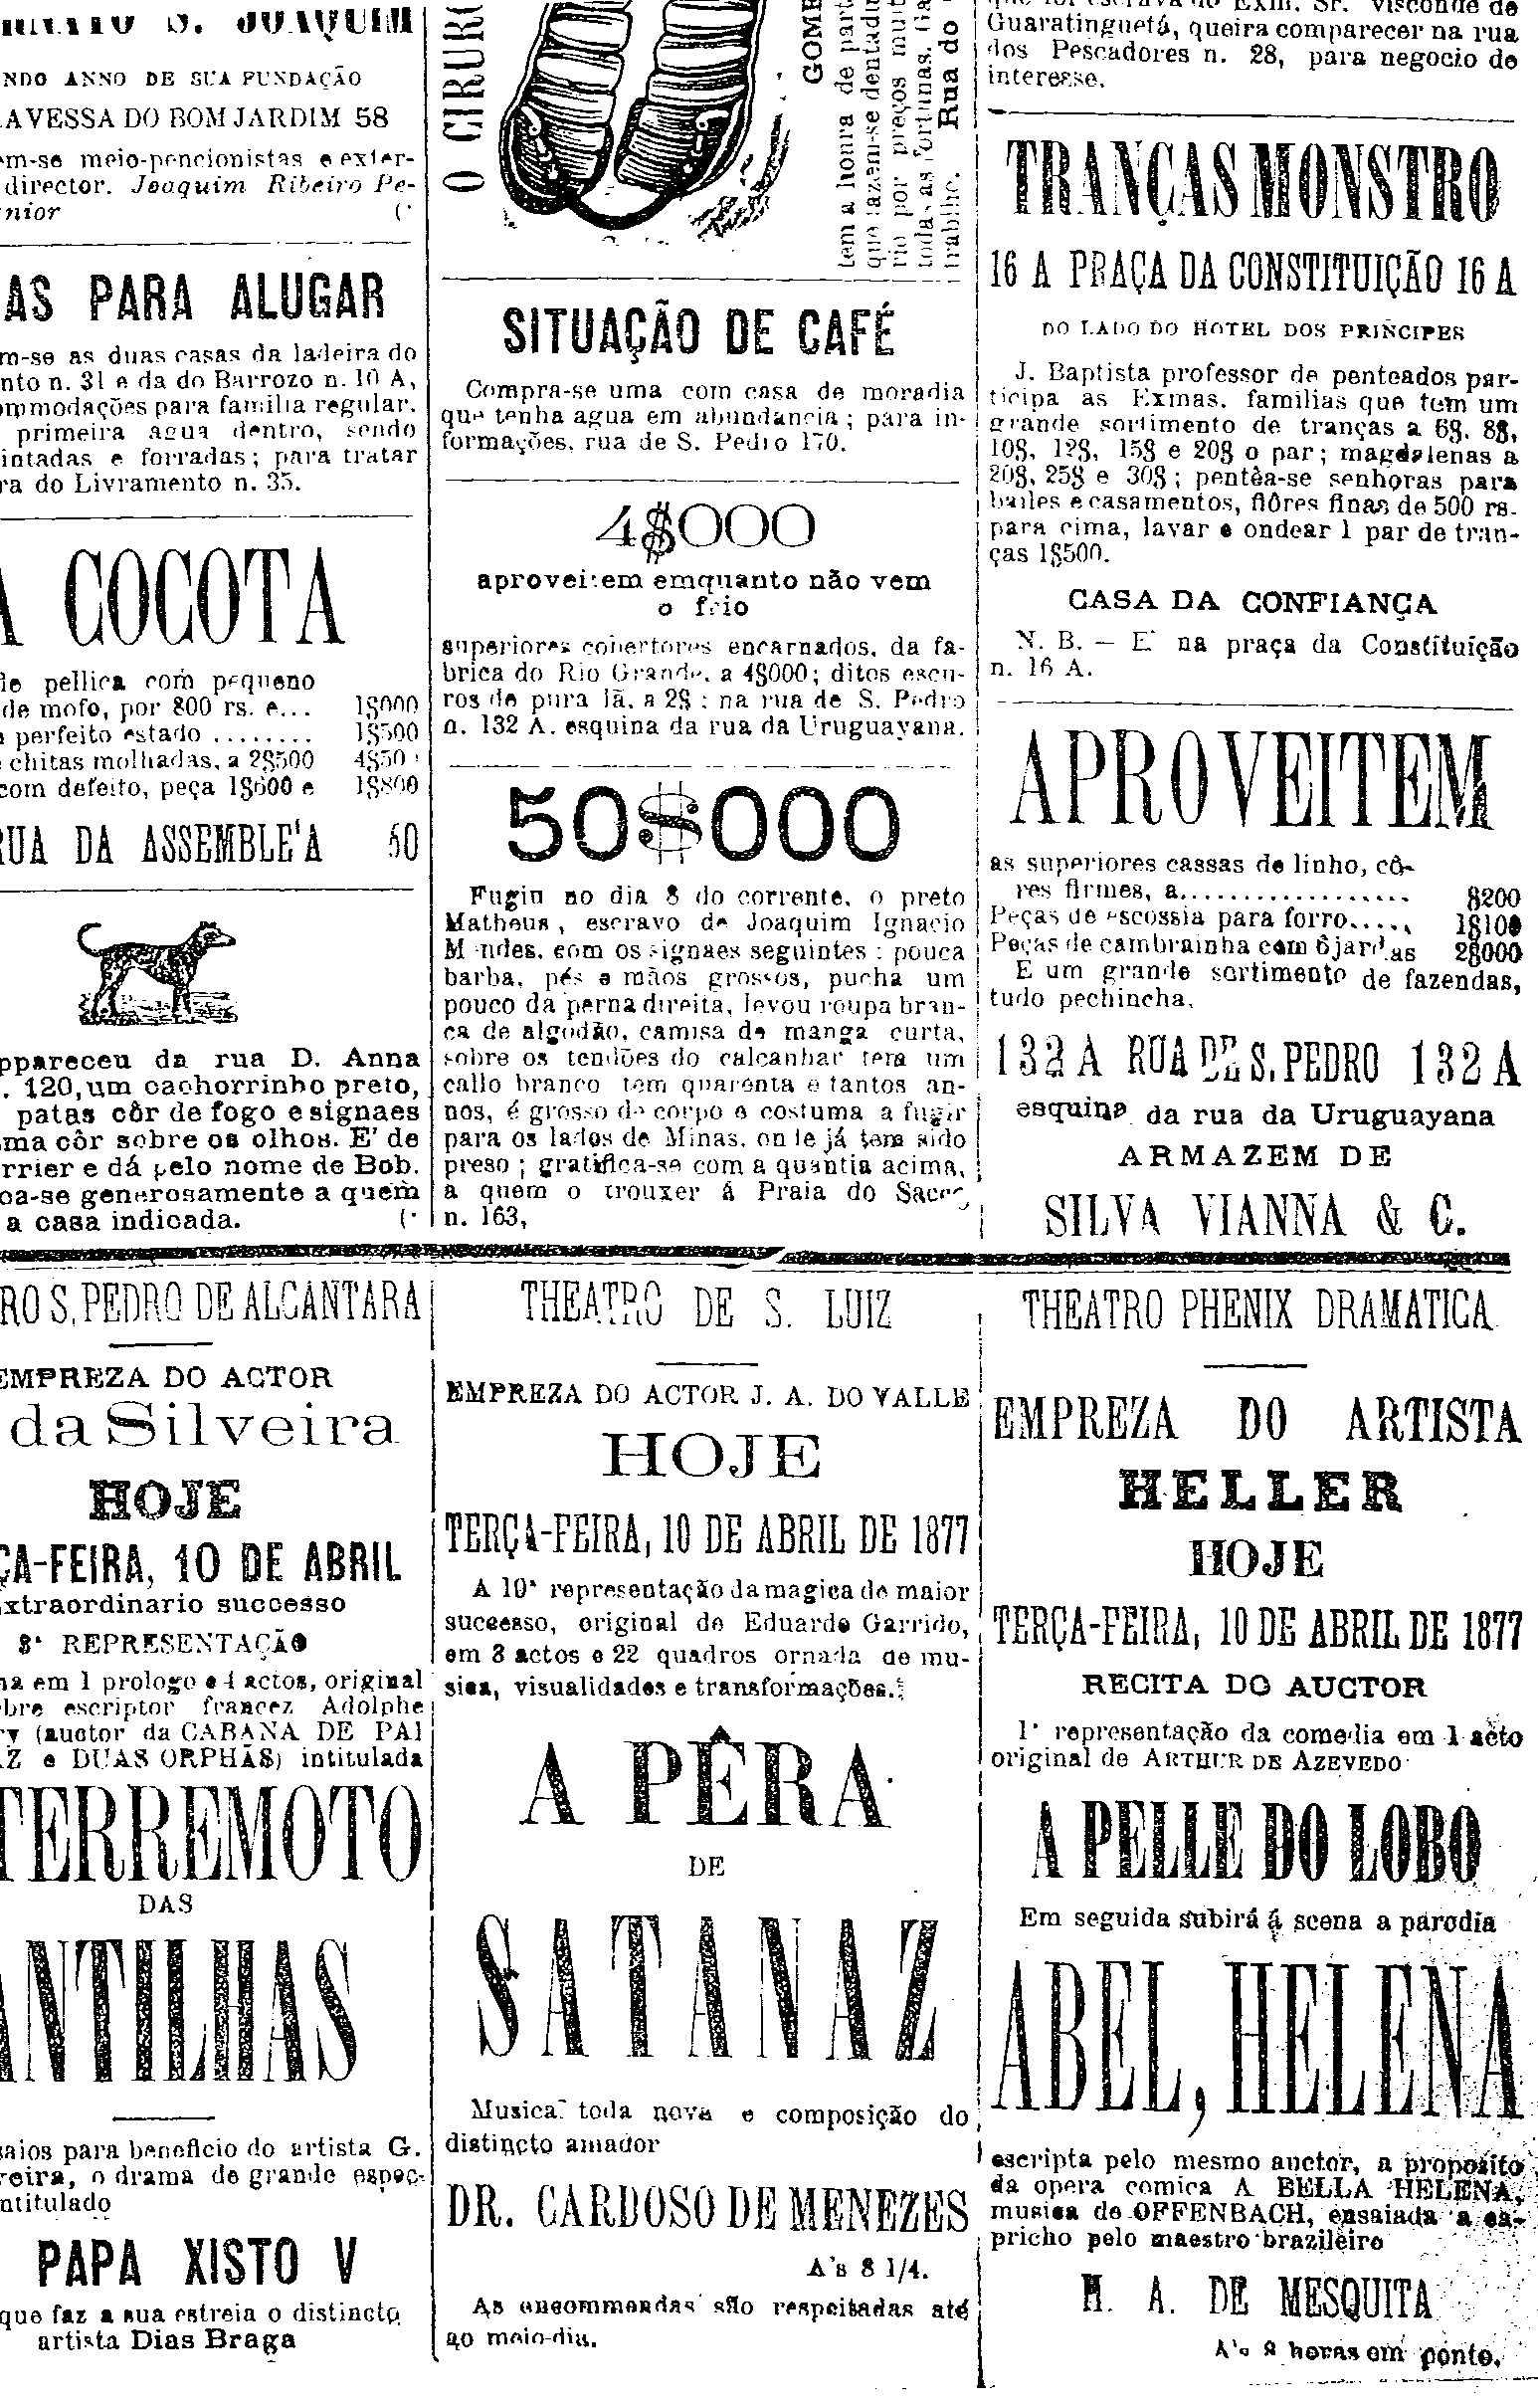
\includegraphics[width=\textwidth]{01.png}\\
{\footnotesize
Anúncio da peça \textit{A pele do lobo}, na \textit{Gazeta de Notícias},\\ em
10 de abril de 1877.}
\end{center}
\end{figure}

\part[A pele do lobo e outras peças]{\textsc{a pele do lobo}\break \textsc{e outras peças}}
\chapter[Amor por Anexins]{Amor por Anexins\subtitulo{Entreato cômico}}
\hedramarkboth{Amor por Anexins}{Artur Azevedo}
\medskip

\textit{Esta farsa, entremez, entreato, ou que melhor nome tenha
em juízo, o meu primeiro trabalho teatral, foi escrito há mais de
sete anos, no Maranhão, para as meninas Riosa, que a
representaram em quase todo o Brasil e até em Portugal. Pô"-la em
música e em boa música, Leocádio Raiol; mas ultimamente
representaram"-na sem ela Helena Cavalier e Silva Pereira:
desencaminhara"-se a partitura. Tem agora nova música, e não
inferior, de Carlos Cavalier.}

\castpage

\cast{Isaías}{solteirão}

\cast{Inês}{viúva}

\cast{Um Carteiro}

\vfill
A cena passa"-se no Rio de Janeiro.

Época, atualidade.

\pagebreak 
\newactnamed{Ato único}

\stagedir{Sala simples, janela à esquerda, portas ao fundo e à direita. Mesa à esquerda
com preparos de costura. Num dos cantos da sala uma talha
d’água. Cadeiras.}

\newscenenamed{Cena I}

\stagedir{\textsc{Inês}}

\repl{Inês} \paren{Cose sentada à mesa, e olha para a rua, pela janela.}  Lá
está parado à esquina o homem dos anexins! Não há meio de ver"-me livre
de semelhante cáustico. Ora eu, uma viúva, e, de mais a mais com promessa de
casamento, havia de aceitar para marido aquele velho! Não vê! E ninguém o tira
dali! Isto até dá que falar à vizinhança\ldots\ \paren{Desce à boca de cena.}

{\smallskip\raggedleft\itshape Copla\footnote{ Versos a serem cantados pelos atores em cena.}\par}
\begin{verse}
Eu, que gosto, perdido\\
Tenho casamentos mil,\\
Com mais de um belo marido,\\
Garboso, rico e gentil,\\
De um velho agora a proposta,\\
Meu Deus! Devia aceitar?\\
Demais um velho que gosta\\
De assim tão jarreta andar!\\
\quad Nada! Nada!\\
\quad Não me agrada!\\
Quero um marido melhor!\\
É bem mau não ser casada,\\
Mas mal casada é pior.\\
\end{verse}

Ainda hoje escreveu"-me uma cartinha, a terceira em que me fala de amor, e a
segunda em que me pede em casamento. \paren{Tira uma carta da algibeira.}
Ela aqui está. \paren{Lê.} “Minha bela senhora. Estimo que estas duas regras vão
encontrá"-la no gozo da mais perfeita saúde. Eu vou indo como Deus é servido.
Antes assim que amortalhado. Venho pedi"-la em casamento pela segunda vez. Ruim é
quem em ruim conta se tem, e eu que não me tenho nessa conta. Jamais senti por
outra o que sinto pela senhora; mas uma \mbox{vez é} a primeira.” \paren{Declamando.}
Que enfiada de anexins! Pois é o mesmo homem a falar! \paren{Continua a
ler.} “Tenho uns cobres a render; são poucos, é verdade, mas de hora em hora
Deus melhora, e mais tem Deus para dar do que o diabo para levar. Não devo nada a ninguém, e quem não
deve não teme. Tenho boa casa e boa mesa, e onde come um comem dois. Irei saber
da resposta hoje mesmo. Todo seu,
Isaías.” \paren{Guardando a carta.} Está bem aviado, Senhor Isaías!  Vou às
compras; é um excelente meio de me ver livre de vossemecê e de seus
anexins. Vou preparar"-me. \paren{Sai pela porta da direita.  Pausa.}

\newscenenamed{Cena II} 

\stagedir{\textsc{[Isaías]}}

\repl{Isaías} \paren{Deita com precaução a cabeça pela porta do fundo.} Porta
aberta, o justo peca.
\paren{Avançando na ponta dos pés.} A ocasião faz o ladrão. Preciso estudar o
gênio desta mulher: antes que cases, olha o que fazes. Dois gênios iguais não
fazem liga; se a pequena não me sai ao pintar, para cá vem de carrinho. É
preciso olhar para o futuro: quem para adiante não olha atrás fica; quem cospe
para o ar cai"-lhe na cara, e quem boa cama faz nela se deita. Resolvi casar"-me,
mas bem sei que casar não é casaca. Alguém dirá que resolvi um pouco tarde,
porém, mais vale tarde que nunca. Deus ajuda a quem madruga, é verdade; mas nem
por muito madrugar se amanhece mais cedo. Procurei uma mulher como quem procura
ouro. Infeliz até ali! Vi"-as a dar com um pau: bonitas, que era um louvar a Deus
de gatinhas; mas\ldots\ nem tudo o que luz é ouro; feias também que era um Deus
nos acuda; mas muitas vezes donde não se espera daí é que vem. Quem porfia mata
caça dizia com meus botões, e não foi nada, que enquanto o diabo esfrega um
olho, cá a dona encheu"-me\ldots\ o olho. Pois olhem que não me passou camarão
pela malha\ldots\ Esta é viúva e costureira\ldots\ Estou pelo beicinho, e creio
que estou servido. Quem já deu não tem para dar, é certo; mas, ora adeus!
quem muito quer muito perde. Já tomei informações a seu respeito: foram as
melhores possíveis; mas como o saber não ocupa lugar, e mais vale um tolo no seu
que um avisado no alheio, observei"-a. Eu sou como
São Tomé: ver para crer. Vi"-a andar sempre sozinha\ldots\ e nada de pândegas!
Dize"-me com quem andas, dir"-te"-ei as manhas que tens.
\paren{Examinando a casa.} Boa dona"-de"-casa parece ser! Asseio e simplicidade.
Pelo dedo se conhece o gigante. Há de ser o que Deus quiser: o casamento e a
mortalha no céu se talham. \paren{Reparando.} Ai, que ela aí vem!
\paren{Perfilando"-se.} Coragem, Isaías! Lembra"-te de que um homem\ldots\
\paren{Atrapalhando"-se.} é um gato e um bicho é um homem!
Disse asneira\ldots


\newscenenamed{Cena III}

\stagedir{\textsc{Isaías} e \textsc{Inês}}

\repl{Inês} \paren{Vem pronta para sair, ao ver Isaías assusta"-se e quer fugir.} Ai!

\repl{Isaías} \paren{Embargando"-lhe a passagem.}  Ninguém deve correr sem ver
de quê.

\repl{Inês}  Que quer o senhor aqui?

\repl{Isaías}  Vim em pessoa saber da resposta de minha carta: quem quer vai e
quem não quer manda; quem nunca arriscou nunca perdeu nem ganhou; cautela e
caldo de galinha\ldots

\repl{Inês} \paren{Interrompendo"-o.} Não tenho resposta alguma que dar!
Saia, senhor!

\repl{Isaías}  Não há carta sem resposta\ldots

\repl{Inês} \paren{Correndo à talha e trazendo um púcaro cheio d’água.} Saia,
quando não\ldots

\repl{Isaías} \paren{Impassível.}  Se me molhar, mais tempo passarei a seu
lado; não hei de sair molhado à rua. Eh! Eh! Foi buscar lã e saiu
tosquiada\ldots

\repl{Inês}  Eu grito!

\repl{Isaías}  Não faça tal! Não seja tola, que quem o é para si \mbox{pede a} Deus
que o mate e ao diabo que o carregue! Não exponha a sua boa reputação! Veja que
sou um rapaz; a um rapaz nada fica mal\ldots

\repl{Inês}  O senhor, um rapaz?! O senhor é um velho muito idiota e muito
impertinente!

\repl{Isaías}  O diabo não é tão feio como se pinta\ldots

\repl{Inês}  É feio, é!\ldots

\repl{Isaías}  Quem o feio ama bonito lhe parece.

\repl{Inês}  Amá"-lo eu?! Nunca\ldots

\repl{Isaías}  Ninguém diga: desta água não beberei\ldots

\repl{Inês}  É abominável! Irra!

\repl{Isaías}  Água mole em pedra dura, tanto dá\ldots

\repl{Inês}  Repugnante!

\repl{Isaías}  Quem espera sempre alcança.

\repl{Inês}  Desengane"-se!

\repl{Isaías}  O futuro a Deus pertence!

\repl{Inês}  Há alguém que me estima deveras\ldots

\repl{Isaías}  Esse alguém \paren{naturalmente} sou eu.

\repl{Inês}  Isso era o que faltava! \paren{Suspirando.} Esse alguém\ldots

\repl{Isaías}  Quem conta um conto, acrescenta um ponto\ldots

\repl{Inês}  Esse alguém é um moço tão bonito\ldots\ de tão boas
qualidades\ldots

\repl{Isaías}  Quem elogia a noiva\ldots

\repl{Inês}  O senhor forma com ele um verdadeiro contraste.

\repl{Isaías}  Quem desdenha quer comprar\ldots

\repl{Inês}  Comprar! Um homem tão feio!\ldots

\repl{Isaías}  Feio no corpo, bonito na alma.

\repl{Inês} \paren{Sentando"-se.}  Deus me livre de semelhante marido!

\repl{Isaías}  Presunção e água benta cada qual toma a que quer\ldots
\paren{Senta"-se também.}

\repl{Inês} \paren{Erguendo"-se.}  Ah, o senhor senta"-se? Dispõe"-se a ficar! Meu
Deus, isto foi um mal que me entrou pela porta!

\repl{Isaías} \paren{Sempre impassível.}  Há males que vêm para bem.

\repl{Inês}  Temo"-la travada.

\repl{Isaías}  Venha sentar"-se a meu lado. \paren{Vendo que Inês senta"-se longe
dele.} Se não quiser, vou eu\ldots\ \paren{Dispõe"-se a aproximar a cadeira.}

\repl{Inês}  Pois sim! Não se incomode! \paren{Faz"-lhe a vontade.} Não há
remédio!

\repl{Isaías} \paren{Chegando mais a cadeira.}  O que não tem remédio remediado
está.

\repl{Inês} \paren{Afastando a sua.} O que mais deseja?

\repl{Isaías}  Diga"-me cá: o seu noivo? \ldots\ \paren{Faz"-lhe uma cara.}

\repl{Inês}  Não entendo.

\repl{Isaías}  Para bom entendedor meia palavra basta\ldots

\repl{Inês}  Mas o senhor nem meia palavra disse!

\repl{Isaías}  Pergunto se\ldots\ fala francês\ldots

\repl{Inês}  Como?

\repl{Isaías}  Ora bolas! Quem é surdo não conversa!

\repl{Inês}  Mas a que vem essa pergunta?

\repl{Isaías} \paren{Naturalmente.}  Quem pergunta quer saber.

\repl{Inês}  Ora!

\repl{Isaías} \paren{Sentencioso.}  Dois sacos vazios não se podem ter de pé.

\repl{Inês}  Essa teoria parece"-se muito com o senhor.

\repl{Isaías}  Por quê?

\repl{Inês}  Porque já caducou também.

\repl{Isaías} \paren{Formalizado.}  Então eu já caduquei, menina?  Isso é
mentira.

\repl{Inês}  É verdade.

\repl{Isaías}  Não é.

\repl{Inês}  É.

\repl{Isaías}  Pois se é, nem todas as verdades se dizem.  \paren{Ergue"-se e
passeia.}

\repl{Inês}  Ah! O senhor zanga"-se? É porque quer; não me viesse dizer tolices!
\paren{Ergue"-se.}

\repl{Isaías} \paren{Interrompendo o seu passeio, solenemente.} Na casa em
que não há pão, todos ralham, ninguém tem razão.

\repl{Inês}  Ora! Somos ainda muito moços!

\repl{Isaías}  Quem? Nós?

\repl{Inês} \paren{De mau humor.}  Não falo do senhor: falo dele\ldots

\repl{Isaías}  Ah! Fala dele\ldots

\repl{Inês}  Havemos de trabalhar um para o outro\ldots

\repl{Isaías}  É bom, é: Deus ajuda a quem trabalha.

{\smallskip\raggedleft\itshape Canto\par}
\begin{verse}
\fala{Inês}\\
Sem desgosto viveremos,\\
Seremos ricos, talvez;\\
Muitos morgados teremos\ldots

%\vfil\pagebreak
\fala{Isaías}\\
Mas um só de cada vez\ldots\\
\paren{Zangado.} A faceira\\
Talvez convidar"-me queira\\
Para padrinho de algum!
\end{verse}

\repl{Inês}  E não suponha que, apesar de pobre, não me faça bonitos presentes
o meu noivo.

\repl{Isaías}  É! Quem cabras não tem e cabritos\ldots

\repl{Inês}  Insulta"-o?

\repl{Isaías}  Cão danado, todos a ele! Pois eu havia de insultá"-lo, senhora?

\repl{Inês}  Se estivesse calado\ldots

\repl{Isaías}  Sim, senhora: em boca fechada não entram mosquitos\ldots\ Mas é
que o seu futurozinho me interessa\ldots

\repl{Inês}  Muito obrigada. \paren{Senta"-se.}

\repl{Isaías}  Não há de quê. Se bem que eu não seja nenhum Matusalém, estou no
caso de lhe dar conselhos. Ouça"-me; quem me avisa meu amigo é; quem à boa árvore
se chega boa sombra o cobre.

\repl{Inês}  Mesmo por já estar no caso de me dar conselhos, é que o não quero
para marido.

\repl{Isaías}  Se eu fosse jovem, não me havia de aceitar, por estar no caso de
os receber. Preso por ter cão e preso por não ter!\ldots

\repl{Inês}  Não desejo enviuvar de novo\ldots

\repl{Isaías}  Vaso ruim não quebra\ldots

\repl{Inês}  Desengana"-se, senhor: não são os seus ditados que me hão de fazer
mudar de resolução! \paren{Passeia.} Oh!

\repl{Isaías} \paren{Acompanhando"-a.} Talvez façam, talvez!\ldots\ Devagar se
vai ao longe\ldots\ Muito tolo é quem se cansa\ldots\ \paren{Inês volta"-se, param defronte um do outro.} Menina,
antes só do que mal acompanhado\ldots\ Olhe que o pior cego é aquele que não
quer ver\ldots

\repl{Inês} \paren{À parte.}  Vou pregar"-lhe uma peta.  \paren{Alto.} Mas se me
faltasse esse noivo, outros rapazes há que me têm feito pé"-de"-alferes.

\repl{Isaías}  Águas passadas não movem moinhos!

\repl{Inês}  E entre eles\ldots

\repl{Isaías} O passado! passado!

\repl{Inês}  Não me interrompa!\ldots\ E entre eles há um ricaço que em outro
tempo\ldots

\repl{Isaías} O tempo que vai não volta!

\repl{Inês}  Não me interrompa, já disse! E entre eles há um ricaço que noutro
tempo se esqueceu da promessa\ldots

\repl{Isaías}  O prometido é devido!

\repl{Inês}  Ai, mau!\ldots\ se esqueceu da promessa que me havia feito; mas
que está outra vez pelo beicinho\ldots

\repl{Isaías}  Cesteiro que faz um cesto faz um cento\ldots \paren{Movimento
de Inês. Com força.} Se tiver verga e tempo! E quem é esse\ldots\ ricaço?

\repl{Inês}  É segredo.

\repl{Isaías}  Segredo em boca de mulher é manteiga em nariz\ldots\ \paren{A um
gesto de Inês} de homem! Mas faz bem, faz bem: o segredo é a alma do
negócio\ldots

\repl{Inês}  O senhor tem na cabeça um moinho de adágios! Passa!\ldots

\repl{Isaías}  O que abunda não prejudica.

\repl{Inês}  Bem! Para maçadas basta. Mude"-se!

\repl{Isaías}  Os incomodados é que se mudam.

\repl{Inês}  Mas eu estou em minha casa, senhor!

\repl{Isaías}  Descobriu mel de pau!

\repl{Inês}  Irra! Que homem sem"-vergonha!

\repl{Isaías} \paren{Examinando cinicamente a costura.}  Quem não tem vergonha
todo o mundo é seu.

\repl{Inês}  Se o meu noivo o visse aqui! Ele, que jurou dar cabo do primeiro
rival que\ldots

\repl{Isaías}  Cão que ladra não morde\ldots\ E eu sou homem!\ldots\ tenho
força\ldots\ E contra a força não há resistência!\ldots

\repl{Inês} \paren{Irônica.}  Ora, por quem é, não faça mal ao pobre moço, sim?

\repl{Isaías}  Faço!\ldots\ Quem o seu inimigo poupa às mãos lhe morre.  Julga
que não estou falando sério? Uma coisa é ver a outra\ldots

\repl{Inês} \paren{No mesmo.}  Ora não faça tal.

\repl{Isaías}  Faço! Isto é tão certo como dois e três serem cinco. São favas
contadas.
Quem não quiser ser lobo não lhe vista a pele!

\repl{Inês}  Mas sabe que ele é valente?

\repl{Isaías}  Também eu sou! Cá e lá más fadas há! Duro com duro não faz bom
muro, e dois bicudos não se beijam!

\repl{Inês}  Ponha"-se ao fresco, preciso sair; tenho que fazer lá fora.

\repl{Isaías}  E eu tenho que fazer cá dentro. Um dia bom mete"-se em casa.
\paren{Pausa.} Olhe, senhora, olhe bem para mim, acha"-me feio: não acha?

\repl{Inês}  Ai, ai, ai!\ldots

\repl{Isaías}  Eu também acho, e feliz é o doente que se conhece. Mas muitas
vezes as aparências enganam e o hábito não faz o monge. Experimente e verá.
\paren{Suplicante.} Case comigo.

\repl{Inês}  Gentes!

\repl{Isaías}  Ah! se fôssemos casadinhos, outro galo cantaria! Por exemplo: em
vez de sair agora à rua, com este sol de matar passarinho, mandava"-me a mim, ao
seu maridinho\ldots

\repl{Inês} \paren{Arremedando"-o.} Ao seu maridinho\ldots\ \paren{À parte.}
Oh! Que ideia! Vou me ver livre dele. \paren{Alto.} Então, sem sermos casados,
não pode prestar"-me um pequeno serviço?

\repl{Isaías}  Conforme o serviço: ponha os pontos nos \textit{ii}.

\repl{Inês}  Se me fosse comprar três metros de escumilha. Olhe\ldots\ Aqui tem
a amostra\ldots\ No armarinho do Godinho\ldots\ Sabe onde é?

\repl{Isaías}  Sei; mas quando não soubesse? Quem tem boca vai a Roma.

\repl{Inês}  Está contrariado?

\repl{Isaías}  O que vai por gosto regala a vida.

\repl{Inês}  Tome o dinheiro.

\repl{Isaías}  Nada\ldots\ não é preciso\ldots\ \paren{Vai saindo e estaca.}
Diabo! não me lembra um ditado a propósito! \paren{Sai.}

\newscenenamed{Cena IV} 

\stagedir{\textsc{[Inês]}}

\repl{Inês}  Está bem aviado\ldots\ Quando voltares, hás de achar a porta
fechada. 
Safa! Que maçador! Agora, tratemos de sair: são mais que horas. \paren{Aparece à
porta um carteiro.}

\newscenenamed{Cena V}

\stagedir{\textsc{Inês, o Carteiro}}

\repl{O Carteiro}  Boa tarde, minha senhora.

\repl{Inês}  Boa tarde. O que deseja?

\repl{O Carteiro}  Aqui tem esta carta\ldots\ é da caixa urbana\ldots

\repl{Inês}  Uma carta? \paren{Recebendo a carta, consigo.} De quem será?
\paren{Ao carteiro.} Obrigada.

\repl{O Carteiro}  Não há de quê, minha senhora. Passe muito bem!

\repl{Inês} Adeus. \paren{O Carteiro sai.}

\newscenenamed{Cena VI} 

\stagedir{\textsc{[Inês]}}

\repl{Inês}  Ah! A letra é de Filipe. Faz bem em escrever"-me o ingrato! Há doze
dias que nos não vemos\ldots\ \paren{Abre a carta e lê. Jogo de fisionomia.}
“Inês.  Peço"-te perdão por ter dado causa a que perdesses comigo o teu tempo.
Ofereceram"-me um casamento vantajoso, e não soube recusar. Ainda uma vez perdão!
Falta"-me o ânimo para dizer"-te mais alguma coisa.
Dentro em uma semana estarei casado. Esquece"-te de mim --- Filipe.”
\paren{Declamando.} Será possível! Oh! Meu Deus! \paren{Relendo.} Sim\ldots\ cá
está\ldots\ é a sua letra\ldots\ \paren{Depois de ter ficado pensativa um
momento.} Ora, adeus. Eu também não gostava dele lá essas coisas\ldots\ Digo
mais, antes o
Isaías; é mais velho, mais sensato, tem dinheiro a render, e Filipe acaba de me
provar que o dinheiro é tudo nestes tempos. Espero aqui o Isaías com o meu “sim”
perfeitamente engatilhado! Oh! O dinheiro\ldots

\begin{verse} 
Louro dinheiro, soberano esplêndido,\\*
Força, Direito, Rei dos reis, Razão.\\*
Que ao trono teu auriluzente e fúlgido\\*
Meus pobres hinos proclamar"-te vão.\\! 

Do teu poder universal, enérgico,\\*
Ninguém se atreve a duvidar! Ninguém!\\*
Rígida mola desta imensa máquina,\\*
Fácil conduto para o eterno bem!\\!

Aos teus acenos, Deus antigo e déspota,\\*
Aos teus acenos, Deus moderno e bom,\\*
Caem virtudes e se exaltam vícios!\\*
Todos te almejam precioso dom!\\!

Inda hás de ser o derradeiro ídolo,\\
Inda hás de ser a só religião,\\
Louro dinheiro, soberano esplêndido,\\
Força, Dinheiro, Rei dos reis, Razão!\ldots
\end{verse}

\newscenenamed{Cena VII}

\stagedir{\textsc{Inês, Isaías}}

\repl{Isaías} \paren{Entrando.}  Quem canta seus males espanta.

\repl{Inês}  Já de volta! O senhor foi a correr!

\repl{Isaías}  Nada! Quem corre cansa. Encontrei outro armarinho mais
perto\ldots

\repl{Inês} \paren{Tomando a fazenda.}  Muito obrigada. Quanto custou?

\repl{Isaías}  Um pau por um olho. Mil e duzentos o metro\ldots

\repl{Inês}  Pois olhe: o outro vende mais barato.

\repl{Isaías}  O barato sai caro, e mais vale um gosto do que quatro vinténs.

\repl{Inês}  Regateou?

\repl{Isaías}  Regatear! Para quê? Mais tem Deus para dar do que o diabo para
tomar.

\repl{Inês}  Já vejo que é tão pródigo de dinheiro como de anexins!

\repl{Isaías}  Da pataca do sovina o diabo tem três tostões e dez réis. Poupado
sim, sovina não.
Eu cá sou assim! Nem tanto ao mar nem tanto à terra. Tenho um só defeito: quero
casar"-me. Cada louco com sua mania.

{\smallskip\raggedleft\itshape Canto\par}
\begin{verse} 
Há sido um gato sapato;\\
Preciso do casamento!\\
O maldito celibato\\
Não é viver, é tormento.

Quero honesta rapariga\\
Entre as belas procurar,\\
Muito embora o mundo diga:\\
Quem já andou não tem pra andar\ldots

A existência de casado\\
Talvez venturas me traga,\\
Se diz verdade o ditado:\\
Amor com amor se paga.

Se eu for constante e fervente,\\
Ela tudo isso será;\\
Se eu amá"-la eternamente,\\
Ela também me amará!

Eu escravo e a esposa escrava,\\
Viveremos sem desgosto;\\
Uma mão a outra lava\\
E ambas lavam o rosto!\ldots
\end{verse}

Faço"-lhe pela milésima vez o meu pedido. Nem todos os dias há carne gorda. A
senhora falou"-me em um apaixonado. Por onde andará ele? Eu estou aqui, e mais
vale um pássaro na mão do que dois a voar.

\repl{Inês} \paren{À parte.}  Levemos a coisa com jeito.  \paren{Alto.} O
senhor\ldots\ \paren{Com uma ideia.} Ah!

\repl{Isaías}  Oh!

\repl{Inês}  Já viu representar \textit{As pragas do Capitão}?

\repl{Isaías}  Não, senhora. De pragas ando eu farto.

\repl{Inês}  Era um militar que praguejava muito. A senhora que ele amava deu"-lhe a mão de esposa, mas depois de estabelecer"-lhe a condição de não praguejar
durante meia hora.

\repl{Isaías}  Falo em alhos, a senhora responde com bugalhos!

\repl{Inês}  Já lá vamos aos alhos: aceito a sua proposta.

\repl{Isaías} \paren{Impetuosamente.}  Aceita?

\repl{Inês}  Sim, senhor.

\repl{Isaías} \paren{Incrédulo.}  Qual! Quando a esmola é muita, o pobre
desconfia\ldots

\repl{Inês}  Mas imponho também a minha condição\ldots

\repl{Isaías}  Imponha: manda quem pode.

\repl{Inês}  Se conseguir levar meia hora sem\ldots

\repl{Isaías}  Sem praguejar?\ldots

\repl{Inês}  Não! Sem dizer um anexim! Se conseguir, é sua a minha mão.

\repl{Isaías}  Deveras?

\repl{Inês} \paren{Sentando"-se.}  Deveras.

\repl{Isaías}  Mas eu posso estar calado?

\repl{Inês}  Como assim?! Era o que faltava! Há de falar pelos cotovelos!

\repl{Isaías}  Isso é um pouco difícil: o costume faz lei\ldots

\repl{Inês}  Ai, que escapou"-lhe um!

\repl{Isaías}  Pois o que quer? A continuação do cachimbo\ldots

\repl{Inês}  Faz a boca torta, já duas vezes.

\repl{Isaías}  Nas três o diabo as fez.

\repl{Inês}  Ai, ai, ai! Vamos muito mal!

\repl{Isaías}  Mas não tínhamos ainda entrado em campo\ldots\ Aqueles foram
ditos de propósito. Agora sim! Agora é que são elas!

\repl{Inês}  Outro!

\repl{Isaías}  Protesto! “Agora é que são elas” nunca foi anexim. A César o que
é de César!

\repl{Inês}  O senhor vai perder\ldots\ Olhe: são duas horas. \paren{Aponta para um
relógio que deve estar sobre a mesa.} Aceita o desafio? \paren{Pausa.} Bem. Quem
cala consente\ldots

\repl{Isaías}  Ah! Agora é a senhora quem os diz! Virou"-se o feitiço contra o
feiticeiro\ldots

\repl{Inês}  Ai, ai!

\repl{Isaías}  Foi engano.

\repl{Inês}  Dos enganos comem os escrivães. \paren{Pausa.} Então?  Diga alguma
coisa\ldots

\repl{Isaías}  O que hei de dizer\ldots\ senão\ldots\ que gosto muito da
senhora\ldots\ e\ldots

\repl{Inês}  Pois diga: vai tantas vezes o cântaro à fonte, que lá fica.

\repl{Isaías}  Não me provoque, senhora, não me provoque!

\repl{Inês}  Cada qual puxa a brasa para sua sardinha\ldots

\repl{Isaías} \paren{Agitado.}  Brasa! Sardinha! Oh! que suplício!

\repl{Inês}  O que tem o senhor?

\repl{Isaías}  Nada\ldots\ não tenho nada\ldots\ é que esta proibição me
incomoda\ldots\ Este maldito costume\ldots\ parece que não estou em mim\ldots

\repl{Inês}  Sabe o que mais?

\repl{Isaías}  Vou saber.

%Jorge: conf. esta fala (o ? final) com o original (mudamos!)
\repl{Inês}  Diga o que quiser! Abra a torneira dos anexins, ditados,
rifões, sentenças, adágios e provérbios\ldots\ Fale, fale para aí!

\repl{Isaías}  E a condição?

\repl{Inês}  Caducou. \paren{Dando"-lhe a mão.} Aqui tem: sou sua.

\repl{Isaías} \paren{Contente.}  Minha! \paren{Em outro tom.} E os outros?

\repl{Inês}  Não existem, nunca existiram!

\repl{Isaías}  Pois estou acordado? Se estiver dormindo, deixa"-me estar: não me
acordes.

\repl{Inês}  Está bem acordado.

\repl{Isaías}  Estou?! \paren{Pulando de contente.} Então viva Deus! Viva o
prazer!\ldots\ Trá lá lá rá lá! \paren{Quer abraçá"-la.}

\repl{Inês} \paren{Gritando.}  Alto lá! Mais amor e menor confiança!

\repl{Isaías}  É que o rato nunca comeu mel, quando come\ldots\ \paren{Outro tom.}
Pode"-se dizer este ditadozinho?\ldots

\repl{Inês}  Quantos quiser!

\repl{Isaías} \paren{Concluindo.}  \ldots\ se lambuza!  \paren{Tomando"-lhe as
mãos.} E tu? Amas"-me, meu bem?

\repl{Inês}  Sossegue: o amor virá depois. Seja bom marido e deixe o
barco andar!

\repl{Isaías}  Apoiado. Roma não se fez num dia!

\repl{Inês}  E tenha sempre muita fé nos seus anexins.

\repl{Isaías}  É verdade: o que tem de ser tem muita força. O homem põe\ldots\
e a mulher dispõe!\ldots

\repl{Inês}  Basta! Despeça"-se destes senhores, e vá tratar dos papéis\ldots

\repl{Isaías}  Quem tem boca não manda\ldots\ cantar. Mas, enfim\ldots\ 
\smallskip

\paren{Ao público.} 

{\smallskip\raggedleft\itshape Copla final\par}
\begin{verse} 
Antes que daqui nos vamos,\\
Inês vos dirá quais são\\
Os votos que alimentamos\\
No fundo do coração.  
\end{verse}

\begin{verse}
\fala{Inês}\\
Os votos que neste instante\\
Fazemos nestes confins\\
\paren{Deita a mão sobre o coração.}\\
É que nos ameis bastante\\
Embora por anexins.

\fala{Ambos}\\
Muitas palmas esperamos\\
\quad De vós:\\
Metade para o autor, metade para nós.
\end{verse}

\vspace{1cm}

\begin{center}
\textsc{Cai o pano}
\end{center}


\chapter{A pele do lobo}

\begin{linenumbers}

\textit{Comédia em um ato escrita em 1875 e representada pela primeira vez no Rio de Janeiro, no
Teatro Fênix Dramática, em 10 de abril de 1877.}
\medskip

\hfill A Antonio Fontoura Xavier


\castpage

\cast{Cardoso}{subdelegado}

\cast{Amália}{sua mulher}

\cast{Apolinário}

\cast{Perdigão}

\cast{Jerônimo}

\cast{Manuel Maria}

\cast{Vitorino}

\cast{O Compadre}

\cast{Uma Parte}

\cast{Dois Soldados da polícia}
\vfil

A cena passa"-se no Rio de Janeiro.
Atualidade.
\pagebreak 

\newactnamed{Ato único}
\stagedir{Sala, secretária, relógio de mesa etc. etc.}

\newscenenamed{Cena I}
\stagedir{\textsc{Cardoso, Amália} vestidos para a cerimônia e prontos para sair.}

\repl{Uma Parte\footnote{ Pessoa que faz a queixa de algum crime (dar parte) ao subdelegado. Todas as notas
são da organização.}} \paren{Que logo sai, à porta do fundo.}

\repl{Cardoso} Sim, senhor; sim, senhor! Pode ir com Deus. Descanse, que
hoje mesmo serão dadas as providências que o caso exige.

\repl{Parte} Às ordens de Vossa Senhoria. \paren{Retira"-se.}

\repl{Cardoso} Safa!

\repl{Amália} \paren{Erguendo"-se.}  Deixar"-te"-ão desta vez?

\repl{Cardoso} E metam"-se! \paren{Passeando.}

\repl{Amália}  Hein?

\repl{Cardoso} E metam"-se a servir o país!

\repl{Amália} Para que aceitaste esta maldita subdelegacia?

\repl{Cardoso} \paren{Ainda passeando.} Eu não aceitei: pedi. Mas já tenho dito
um milhão de vezes que os serviços prestados ao país e ao partido pesam muito no
ânimo daqueles que me podem fazer galgar mais um degrau na
escala social.

\repl{Amália} Deixa"-te disso, Cardoso; um degrau dessa tão falada escala social
não vale decerto o sacrifício que te custa essa autoridade de ca"-ca"-ra"-cá. São
uns desfrutadores, eis o que são! Hás de ser pago com um pontapé. Verás!

\repl{Cardoso} Hei de ser promovido na primeira vaga que aparecer. O
Cantidiano está por pouco a bater a bota. Verás se o lugar é ou não é meu!

\repl{Amália} Fia"-te na Virgem e não corras.

\repl{Cardoso} E uma vez que aceitei o cargo\ldots{}

\repl{Amália} A carga, deves dizer.

\repl{Cardoso} Venha com ele o sacrifício. Antes de tudo o dever!

\repl{Amália} Estamos prontos para sair há duas horas.

\repl{Cardoso} \paren{Consultando o relógio de mesa.} Há duas horas e
dois minutos.

\repl{Amália} \paren{Embonecando"-se ao espelho.} Creio que não chegamos a
tempo para o batizado.

\repl{Cardoso} Que remédio terão eles, senão esperar pelos padrinhos?

\repl{Amália} E o carro na porta há tanto tempo!

\repl{Cardoso} Anda com isso, anda com isso! E metam"-se!

\repl{Amália} Hein?

\repl{Cardoso} E metam"-se a servir o país!

\repl{Amália} Vamos. Não percamos mais tempo.

\repl{Cardoso} Vamos. \paren{Vão saindo. Batem palmas.}

\repl{ambos} Bateram.

\repl{Cardoso} Quem é?

\repl{Apolinário} \paren{Fora.} Sou eu.

\repl{Amália} Eu quem?

\repl{Apolinário} \paren{No mesmo.} Um criado de Vossa Senhoria.

\repl{Cardoso} Entre quem é.

\repl{Amália} Temo"-la travada! \paren{Entra Apolinário. Pisa macio e fala
descansado.}

%\vfil\pagebreak 
\newscenenamed{Cena II}

\stagedir{\textsc{Os mesmos} e \textsc{Apolinário}}

\repl{Apolinário} \paren{À porta do fundo.} Dá licença, senhor
subdelegado?

\repl{Cardoso} Entre, senhor. \paren{Vai outra vez pôr o chapéu na
secretária.}

\repl{Apolinário} \paren{Entrando e sentando"-se em uma cadeira que deve estar
no meio da cena.} Não se incomode
Vossa Senhoria. Estou muito bem. Vossa Senhoria como tem passado?

\repl{Cardoso} Bem, obrigado. O que pretende o senhor?

\repl{Apolinário} Sua senhora tem passado bem, senhor subdelegado?

\repl{Amália} Bem, obrigada. O senhor o que pretende?

\repl{Apolinário} Ah! estava aí, minha senhora? Os meninos estão bons?

\repl{Amália} Que meninos, senhor?

\repl{Apolinário} Os seus filhos, minha senhora.

\repl{Amália} Não os tenho. E esta!

\repl{Apolinário} Pois levante as mãos para o céu e dê graças a Nosso Senhor Jesus
Cristo! \paren{Sinais de impaciência em Cardoso e Amália.} Eu tenho três, três!
Todos três machos, felizmente. Mas que consumição! Que canseira! Quando não está
um doente, está outro; quando não está outro, está outro; quando não está
nenhum, está a mãe; quando não está a mãe, está o pai. Às vezes estão, filhos e
pais, todos doentes. É preciso chamar a
vizinha para dar"-nos qualquer coisa. É uma lida, minha rica senhora!
Peça a Deus que não lhe dê filhos. Olhe\ldots{} \paren{Mostra a cabeça.} Não vê?

\repl{Amália} O quê? O quê?

\repl{Apolinário} Já estou pintando\ldots{} Ainda anteontem\ldots{} Anteontem
não\ldots{} Quando foi, Apolinário? Segunda\ldots{} terça\ldots{} Foi anteontem
mesmo\ldots{}  Eu tinha acabado de tomar o meu banhinho e de ouvir minha
missinha\ldots{}

\repl{Cardoso} \paren{Interrompe"-o.}  Meu caro senhor, tomo a liberdade
de preveni"-lo que temos muita pressa e não
podemos perder tempo. Íamos saindo justamente quando o senhor entrou\ldots{}

\repl{Apolinário} \paren{Erguendo"-se.} Nesse caso, senhor doutor\ldots{}

\repl{Cardoso} Perdão; não sou doutor.

\repl{Apolinário} Fica para outro dia\ldots{} Eu vinha dar minha queixa, mas\ldots{}
\paren{Cumprimenta.} Senhor doutor\ldots{} minha
senhora\ldots{} \paren{Vai saindo.}

\repl{Cardoso} Venha cá, senhor: já agora diga o que pretende.

\repl{Apolinário} \paren{Voltando"-se e preparando"-se como para um discurso,
com força.}  Senhor subdelegado\ldots{}

\repl{Cardoso} Não é preciso gritar tanto\ldots{}

\repl{Apolinário} Esta noite fui roubado.

\repl{Cardoso} Diga.

\repl{Apolinário} Dezoito cabeças de criação\ldots{} dezoito ou dezenove\ldots{} Ontem
esteve em nossa casa um cunhado
meu, irmão de minha mulher, empregado no Arsenal de Guerra, e não tenho
certeza de que ele levasse alguma
galinha consigo, mas creio que não. Em todo caso, foram dezoito ou
dezenove cabeças, não falando em um
bonito galo de crista, que comprei no mercado, não há quinze dias.

\repl{Cardoso} Muito bem. O senhor chama"-se\ldots{}

\repl{Apolinário} Apolinário, um criado de Vossa Senhoria.

\repl{Cardoso} Apolinário de quê?

\repl{Apolinário} Apolinário da Rocha Reis Paraguaçu \paren{Dando um
cartão.} Olhe, aqui tem Vossa Senhoria meu
nome e morada.

\repl{Cardoso} Bem; pode ir descansado, que serão dadas as providências que o
caso exige.

\repl{Apolinário} \paren{Preparando"-se outra vez para um discurso e elevando
muito a voz.} Ainda não fica nisso,
senhor doutor!

\repl{Cardoso} Já tive ocasião de dizer"-lhe, primeiro, que não é preciso
gritar tanto; segundo, que não sou doutor.

\repl{Apolinário} \paren{Com a mesma inflexão, porém baixinho.} Não fica
nisso. Eu conheço o gatuno!

\repl{Cardoso} E por que estava calado?

\repl{Amália} \paren{Não se podendo conter.} Com efeito, Senhor
Paraguaçu!

\repl{Apolinário} \paren{Atarantado.} Hein! \paren{Falando com cada
vez mais descanso.} Não conheço eu outra coisa!
Chama"-se Jerônimo de tal, um ilhéu, um vagabundo, que foi há tempo
cocheiro de bondes e agora não sai da
venda de seu Manuel Maria, ao qual dizem que vende por um precinho de
amigo, o que\ldots{} \paren{Ação de furtar.}
Vossa Senhoria sabe qual é a venda de seu Manuel Maria? É a que fica
mesmo em frente à casa do meu
cunhado, do mesmo que esteve ontem em nossa casa, e sobre o qual estou
em dúvida se levou ou não alguma
galinha. \paren{A Amália.} Mas que bonito galinho, senhora! Vossa
Senhoria dava oito mil réis por ele com os olhos
fechados\ldots{} Era branco, branquinho, como aqueles patinhos do Passeio
Público. Uma crista escarlate! Que
bonito galo!

\repl{Cardoso} Vamos! Não temos tempo a perder! Faça o favor de sentar"-se
naquela mesa e dar a queixa por
escrito.

\repl{Apolinário} De muito bom gosto, senhor doutor. \paren{Obedece.}

\repl{Cardoso} E o senhor a dar"-lhe! Já lhe disse que não sou doutor.

\repl{Apolinário} Isso é modéstia de Vossa Senhoria.

\repl{Amália} Parece de propósito, Senhor Paraguaçu.

\repl{Cardoso} Deixa"-o lá. \paren{Vai para junto de Amália.} Que
maçador! E metam"-se!

\repl{Amália} Não chegaremos a tempo.

\repl{Apolinário} \paren{À mesa.} Esta pena está escarrapachada, senhor
subdelegado\ldots{}

\repl{Cardoso} Vou dar"-lhe outra\ldots{} Vou dar"-lhe outra\ldots{}

\repl{Amália} Anda\ldots{} Tem paciência\ldots{} Acaba com isso. \paren{Cardoso vai
abrir a secretaria e muda a pena da caneta.}

\repl{Apolinário} Muito obrigado! Que incômodo tem tomado Vossa Senhoria! Mas
também não há quem diga à
boca cheia: “Aquilo é que é um subdelegado! Zelo até ali\ldots{} É o pai das
Partes!”.

\repl{Cardoso} Faça o favor de escrever o que tem de escrever\ldots{}

\repl{Apolinário} Às ordens de Vossa Senhoria. \paren{Escreve.}

\repl{Cardoso} \paren{Voltando para junto de Amália.} Decididamente peço
a demissão!

\repl{Amália} Isso é o que já devias ter feito há muito tempo.

\repl{Cardoso} Olha que é bem difícil suportar uma maçada assim\ldots{} E
metam"-se!

\repl{Amália} Hein?

\repl{Cardoso} E metam"-se a servir o país!

\repl{Amália} Pede a demissão, Cardoso, pede a demissão.

\repl{Apolinário} \paren{Da mesa.} Senhor subdelegado, faça o favor de
me dizer o modo por que devo principiar este
requerimento\ldots{} Em matéria de polícia sou completamente leigo\ldots{} Diga"-me
só o cabeçalho\ldots{} O cabeçalho!
O resto vai\ldots{}

\repl{Cardoso} Ai, Senhor Paraguaçu! O senhor é maçante! Tenho estado a
aturá"-lo há meia hora!

\repl{Amália} \paren{Olhando o relógio.} Há meia hora e sete minutos.

\repl{Cardoso} Estamos muito apressados, meu caro senhor\ldots{} Não posso estar
com isso\ldots{}

\repl{Apolinário} Eu quis retirar"-me quando Vossa Senhoria disse que\ldots{}

\repl{Cardoso} Vamos lá! Escreva no alto --- Ilustríssimo Senhor.

\repl{Apolinário} O Ilustríssimo Senhor --- já cá está.

\repl{Cardoso} Bem \paren{Ditando.} “O abaixo assinado, morador nesta
freguesia, à rua de tal, número tal\ldots{}”

\repl{Apolinário} \paren{Escrevendo.} \ldots{} número treze\ldots{}

\repl{Cardoso} “Queixa"-se a Vossa Senhoria de que, ontem, às tantas horas da
noite\ldots{}”

\repl{Apolinário} “Queixa"-se” é com \textit{x} ou \textit{ch}?

\repl{Amália} Ó céus! \paren{Rindo"-se.}

\repl{Cardoso} Como quiser! Não faço questão de ortografia.

\repl{Apolinário} Vai com \textit{ch}. \paren{Acabando.}\ldots{} “da noite”\ldots{}

\repl{Cardoso} Como está?! \paren{Vendo.} Fulano de tal, tal, tal. Ah!
\paren{Ditando.} “Furtaram"-lhe tantas galinhas\ldots{}”

\repl{Apolinário} \paren{Escrevendo.} \ldots{}``e um galo de crista”\ldots{}
%luis não falta abertura das aspas?

\repl{Cardoso} “\ldots{} as suspeitas de cujo furto faz recair em Fulano de Tal.”
\paren{Consultando o relógio.} E metam"-se!

\repl{Apolinário} \paren{Escrevendo.} “Fulano de tal, vulgo
Barriga"-cheia.” Pronto!

\repl{Cardoso} Na outra linha: “Deus guarde a Vossa senhoria”.

\repl{Apolinário} \ldots{} “a Vossa Senhora”\ldots{}

\repl{Cardoso} Na outra linha: “Ilustríssimo Senhor Subdelegado de tal
freguesia”.

\repl{Apolinário} Pronto.

\repl{Cardoso} Assine.

\repl{Apolinário} \ldots{} “Apolinário da Rocha Reis Paraguaçu.”
\paren{Erguendo"-se.} Pronto.

\repl{Cardoso} Bem; agora pode ir descansado, que serão dadas as providências
que o caso exige.

\repl{Apolinário} Com licença, senhor subdelegado\ldots{} Às ordens de Vossa
Senhoria\ldots{}

\repl{Cardoso} Passe bem.

\repl{Apolinário} Minha senhora\ldots{}

\repl{Amália} Viva. \paren{Volta"-lhe as costas.}

\repl{Apolinário} Sem mais incômodo. \paren{Saída falsa.}

\repl{Cardoso} Safa!

\repl{Amália} Saiamos, saiamos quanto antes! Pode vir outro\ldots{} \paren{Vão
saindo.}

\repl{Apolinário} \paren{Voltando.} Ia"-me esquecendo, senhor
subdelegado\ldots{}

\repl{Cardoso} Outra vez!

\repl{Amália} Assustou"-me até!

\repl{Cardoso} O que mais deseja?

\repl{Apolinário} Hoje, logo depois do almoço, encontrei"-me cara a cara com o
tal Jerônimo!

\repl{Cardoso} Que Jerônimo, senhor?

\repl{Apolinário} O Barriga"-cheia, o tal que me furtou as galinhas\ldots{}

\repl{Cardoso} E o que tenho eu com isso, não me dirá?

\repl{Apolinário} Direi, sim, senhor. Com licença. \paren{Desce à cena e
senta"-se.} Chamei"-o de ladrão! Disse"-lhe assim: “Você é um ladrão!” --- Com licença da senhora\ldots{}

\repl{Amália} E o que tem meu marido com isso?

\repl{Apolinário} É que o sujeito tomou três testemunhas, e diz que me vai
processar por crime de injúrias verbais.

\repl{Cardoso} Mas, enfim, faz favor de me dizer para que voltou cá?

\repl{Apolinário} Vim prevenir a Vossa Senhoria de que\ldots{}

\repl{Cardoso} Vá prevenir ao diabo que o carregue!

\repl{Apolinário} \paren{Levantando"-se.} Senhor, doutor.

\repl{Cardoso} \paren{Gritando.} Já lhe disse que não sou doutor!

\repl{Apolinário} \paren{Imitando"-o.} Isso é modéstia de Vossa senhoria!

\repl{Cardoso} Saia! Ponha"-se ao fresco! Supõe o senhor que sirvo de joguete?

\repl{Apolinário} Mas Vossa Senhoria\ldots{}

\repl{Cardoso} Saia!

\repl{Apolinário} É que\ldots{}

\repl{Amália} Oh! senhor, já é a terceira vez que se lhe diz --- saia.

\repl{Apolinário} Minha senhora, eu\ldots{} \paren{Tornando a sentar"-se, com todo
o sossego.} Com licença\ldots{}

\repl{Amália} Oh! isto é demais!

\repl{Cardoso} Então, não ouve!

\repl{Apolinário} Quero justificar"-me!

\repl{Cardoso} \paren{Ameaçador.} Cuidado, Senhor Paraguaçu!

\repl{Apolinário} Bem, Vossa Senhoria está em sua casa: manda.
\paren{Levantando"-se e cumprimentando.} Às ordens
de Vossa Senhoria.

\repl{Cardoso} Viva! Há mais tempo! \paren{Passeia agitado.}

\repl{Apolinário} Minha senhora\ldots{}

\repl{Amália} Passe bem. \paren{Saída falsa de Apolinário.} Que inferno!
Que inferno! E metam"-se!

\repl{Apolinário} \paren{Voltando.} Acredite, senhor doutor, que eu não
queria de forma alguma\ldots{}

\repl{Cardoso} \paren{Desesperado.} Ah! ele é isso? \paren{Agarra uma
cadeira e levanta"-a, correndo para Apolinário.}

\repl{Amália} \paren{Muito aflita.} Ah! \paren{Suspende o braço de
Cardoso. Ficam todos numa posição dramática.}

\repl{Apolinário} \paren{Com todo o sangue frio.} Tableau.\footnote{ \textit{Tableau}: O final de uma cena;
``quadro'', em francês.}
\paren{Desaparece.}


\newscenenamed{Cena III} 

\stagedir{\textsc{Cardoso} e \textsc{Amália}}

\repl{Cardoso} Vês, Sinhá, vês como um homem se deita a perder?

\repl{Amália} Sim, sim, mas vamos, anda daí!

\repl{Cardoso} \paren{Caindo na cadeira que tinha nas mãos.} E que dor
de cabeça fez"-me este bruto!\ldots{} E metam"-se.

\repl{Amália} Hein?

\repl{Cardoso} E metam"-se a servir o país!

\repl{Amália} Espera\ldots{} vou buscar a garrafinha de água"-flórida.\footnote{
Água de colônia utilizada no século \textsc{xix} para limpar, perfumar e fazer
descarrego.}
\paren{Sai
e volta com a garrafinha.}

\repl{Cardoso} Depressa\ldots{} depressa, Sinhá! \paren{Amália esfrega"-lhe as
frontes com água"-flórida.} Bem\ldots{} basta\ldots{} está
pronto\ldots{} Ai! que ferroadas! Deita a garrafinha em cima da mesa e vamos,
vamos! \paren{Amália deita a garrafinha sobre a mesa e vai dar o braço a seu marido.}

\repl{Amália} Vamos! \paren{Saem e voltam.} Esqueci"-me do leque.
\paren{Entra à direita baixa.}

\repl{Cardoso} \paren{Falando para dentro.} Que demora, Sinhá, que demora!
Ainda há de vir alguém, verás! \paren{Passeia.}
Então não achas esse leque! Ai! minha cabeça! E metam"-se!
\paren{Quebra"-se alguma coisa dentro.} O que foi
isso?! O que foi isso?! \paren{Corre também para a direita baixa.}

\repl{Amália} \paren{Dentro.} O meu frasco de água da Colônia!

\repl{Cardoso} \paren{Dentro.} Que pena!

\repl{Amália} \paren{Dentro.} Ah! cá está o leque! \paren{Voltam à
cena, de braço dado e dirigem"-se para a porta.}

\repl{Cardoso} Já estou suando. \paren{Procura nos bolsos.} Não tenho
lenço.

\repl{Amália} Oh! que maçada! Quanto mais pressa, mais vagar. \paren{Sai
correndo pela direita baixa.}

\repl{Cardoso} E metam"-se, hein! E metam"-se a servir o país!

\repl{Amália} \paren{Voltando com um par de meias na mão.} Toma, toma\ldots{} Apre! 
\paren{Dá"-lho.}

\repl{Cardoso} Isto é um par de meias, Sinhá! Estás a meter os pés pelas
mãos! \paren{Restitui"-lho.}

\repl{Amália} Como está esta cabeça, meu Deus! \paren{Sai e volta com um
lenço.} Toma\ldots{} Vamos\ldots{} Uf!

\repl{Cardoso} Vamos! \paren{Encaminham"-se para a porta. Batem palmas.}

\repl{Ambos} Ah!

\repl{Cardoso} \paren{Fora de si.} Não estou em casa!

\repl{Jerônimo} \paren{Aparecendo, de chapéu na cabeça.} Licença para
um\ldots{}


\newscenenamed{Cena IV} 

\stagedir{\textsc{Os mesmos} e \textsc{Jerônimo}}

\repl{Cardoso} Então é assim que se entra em casa alheia?

\repl{Jerônimo} \paren{Sombrio.} Assim como? A casa da autoridade é uma
repartição pública. \paren{Deita no chão a cinza de um cachimbo; e escarra na parede.}

\repl{Cardoso} E que tal?

\repl{Amália} Vê o que ele quer, Cardoso?

\repl{Jerônimo} Venho preveni"-lo de que é falso o que lhe veio hoje dizer um
tal Paraguaçu, acerca de um furto de
galinhas. É provável que ele lhe dissesse que eu, Jerônimo Linhares,
vulgo Barriga"-cheia, sou o autor desse
furto, como andou por aí dizendo a quem quis ouvi"-lo. É falso!
\paren{Cospe outra vez na parede.}

\repl{Amália} \paren{Empurrando um escarrador com o pé.} Faz favor de
não cuspir no chão\ldots{} Aqui tem o escarrador\ldots{}
\paren{Jerônimo nem olha para Amália.}

\repl{Cardoso} Era só isso? Estou ciente.

\repl{Jerônimo} Não, senhor; por isto só não vinha eu cá, ora viva! Venho
queixar"-me do queixoso por crime de
injúrias verbais. Chamou"-me de ladrão, e se quiser o mais, mande aquela
mulher para dentro. \paren{Cospe outra vez na parede.}

\repl{Cardoso} Pois apresente a queixa e as testemunhas.

\repl{Jerônimo} A queixa aqui está. \paren{Apresenta um papel sujo, que
Cardoso pega com repugnância. Vai à porta do fundo.} Ó compadre! Ó seu Manuel Maria! Ó seu Vitorino? Podem
entrar\ldots{} Nada de cerimônias!

\repl{Cardoso} \paren{A Amália.} O tratante dispõe desta casa como se
fosse sua!

\newscenenamed{Cena V} 

\stagedir{\textsc{Os mesmos, Manuel Maria}, depois \textsc{O Compadre}, depois \textsc{Vitorino}}

\repl{Manuel Maria} \paren{Entrando.} Aqui estou eu!

\repl{Compadre} \paren{Entrando.} E eu\ldots{}

\repl{Vitorino} \paren{Entrando.} E eu\ldots{}

\repl{Amália} Cardoso, dize"-lhes que venham em outro dia\ldots{} \paren{À
Parte.} Como cheiram a cachaça!

\repl{Cardoso} Meus senhores, tenham a bondade de voltar amanhã.

\repl{Jerônimo} Aí vem o maldito sistema da demora e do papelório.

\repl{Cardoso} Cala"-te daí, insolente, que não tens autoridade para fazer
considerações neste lugar\ldots{} Apareçam
terça"-feira ou mesmo amanhã! Mas terça"-feira é melhor, porque é o dia da
audiência. Não posso estar agora
com isto\ldots{} Estamos prontos para sair há muito tempo!

\repl{Amália} Há três horas!

\repl{Cardoso} \paren{Consultando o relógio.} Há três horas e três
minutos!

\repl{Jerônimo} \paren{Cuspindo na parede.} Então, podiam ter dito logo!
Escusava a gente de estar aqui à espera! É isto
sempre! A autoridade vai para a pândega, e o povo que sofra!

\repl{Cardoso} Insolente! Espera que te ensino! \paren{Agarra numa cadeira
que está perto do toucador.}

\repl{Amália} Cardoso! O que vais fazer?!\ldots{}

\repl{Jerônimo} Ah! Ele é isso? \paren{Tira uma faca e deita a correr atrás
de Cardoso. Amália fecha"-se no quarto. As três testemunhas correm atrás de Jerônimo, para retê"-lo. Cardoso
apita.\footnote{ No século \textsc{xix}, a polícia utilizava um apito para chamar ou reunir
os soldados para ação. As pessoas comuns também podiam apitar para chamar a polícia.}}

\repl{Manuel Maria} O que é isto, seu Jerônimo?!

\repl{Compadre} Compadre, tenha mão!

\repl{Vitorino} Não se deite a perder!
\paren{Cardoso continua a apitar. Confusão.}

\repl{Amália} \paren{Grita de dentro.} Aqui d’el"-rei!


\newscenenamed{Cena VI} 

\stagedir{\textsc{Os mesmos} e \textsc{Dois Soldados}}

\repl{Soldados} O que é isto? O que é isto?\ldots{} \paren{Correm todos em redor da cena.}

\repl{Cardoso} Prendam"-no! Prendam"-no! \paren{Jerônimo é afinal preso.}
Levem"-no! \paren{Os Soldados levam o preso.} 
\paren{Saem também as testemunhas.}


\newscenenamed{Cena VII} 

\stagedir{\textsc{Cardoso} e depois \textsc{Amália}}

\repl{Cardoso} \paren{Caindo extenuado em uma cadeira.} Uf!

\repl{Amália} \paren{Entrando.} Feriu"-te o maldito, feriu"-te?

\repl{Cardoso} Creio que não. \paren{Apalpando"-se.} Não feriu, não, Sinhá!
Se não fossem as ordenanças que estavam na
porta, a estas horas estavas viúva!

\repl{Amália} Credo! Viúva!

\repl{Cardoso} Maldita subdelegacia! Maldita a hora em que aceitei semelhante
cargo!

\repl{Amália} Como estás suando! Esta camisa é incapaz de aparecer no
batizado\ldots{}

\repl{Cardoso} É verdade! O batizado! Vou mudar de camisa\ldots{}

\repl{Amália} Mas isso depressa\ldots{} depressa! \paren{Saída falsa de
Cardoso.} Ó Senhor Deus! Isto contado lá se acredita!
É bem feito, senhor meu marido, é bem feito! Quem não quiser ser
lobo, não lhe vista a pele. \paren{Rolo na rua.
Apitos. Gritos. Pancadaria. Amália vai à janela.} Que vejo! Uma
malta de capoeiras!\footnote{ Grupos de capoeiras formados, em sua maioria, por homens
mulatos e negros, que lutavam entre si e com a polícia, utilizando golpes de
capoeira, navalha e bengalas como armas. As maltas foram duramente reprimidas
pela polícia, no final do século \textsc{xix}. Ver Introdução, p.~\pageref{capoeira}.} Cardoso! Cardoso! Não
tardam a entrar\ldots{}

\repl{Cardoso} \paren{Entra em mangas de camisa e com o fitão de
subdelegado.\footnote{ Fita utilizada por delegados e subdelegados, como símbolo do cargo.}} 
O que é isto? \paren{Espirra.} Atchim!
Constipei"-me\ldots{} Atchim! O que é isto? Atchim! \paren{Sai a correr pelo
fundo.}


\newscenenamed{Cena VIII} 

\stagedir{\textsc{Amália}, depois \textsc{Perdigão}}

\repl{Amália} Meu Deus! Hoje parece ser o dia de São Bartolomeu! Se não anda
o diabo solto na cidade, ao menos
nesta freguesia.

\repl{Perdigão} \paren{Entra apressado pelo fundo, vestido para a cerimônia.}
Ó compadre! Ó comadre!

\repl{Amália} Mais uma Parte!

\repl{Perdigão} Deixe"-se de Partes!

\repl{Amália} Meu marido não está\ldots{} \paren{Reparando.} Ah! é o compadre!

\repl{Perdigão} Estamos até estas horas à espera do padrinho e nada!

\repl{Amália} Queixe"-se da maldita subdelegacia, compadre! Estamos vestidos
há três horas\ldots{} \paren{Consultando o relógio.} Há três horas e um quarto\ldots{}

\repl{Perdigão} Ora! Para que foi o compadre buscar sarna para se coçar\ldots{}

\repl{Amália} O compadre não imagina! Quantas vezes, alta noite, está ele
sossegado a dormir, quando, de
repente, é despertado pelas malditas partes\ldots{}

\repl{Perdigão} Por força!

\repl{Amália} \paren{Indo à janela.} Já está aplacado o rolo\ldots{}
\paren{Voltando.} Hoje quase o matam!

\repl{Perdigão} \paren{Dando um salto.} A quem?

\repl{Amália} Ao Cardoso.

\repl{Perdigão} Ah! Ele descia a escada com tanta impetuosidade! Ia em mangas
de camisa e de fitão\ldots{} Olhem que
figura! Espirrava, que era um Deus nos acuda! “Viva!” lhe disse eu; ele,
porém, não me conheceu, apesar de
responder ``\textit{Dominus tecum”},\footnote{ “Deus esteja contigo”, em latim.}
em vez de ``Obrigado!”

\newscenenamed{Cena IX}

\stagedir{\textsc{Os mesmos} e \textsc{Cardoso.}}

\repl{Cardoso} \paren{Entra e cai espirrando em uma cadeira.} Atchim!

\repl{Perdigão} Viva!

\repl{Cardoso} \textit{Dominus te\ldots{}} Quero dizer: obrigado\ldots{} Atchim! Ah! é o
senhor, compadre? Desculpe.

\repl{Perdigão} Já sei de tudo\ldots{} Está mais que desculpado\ldots{} Mas não perca
tempo!

\repl{Amália} Sim, não percamos tempo!

\repl{Cardoso} Vamos! \paren{Ergue"-se e deita o chapéu.} Estou pronto!

\repl{Perdigão} Em mangas de camisa, compadre?

\repl{Cardoso} É verdade! \paren{Corre ao quarto e volta vestindo a
casaca.}

\repl{Amália} De fitão, Cardoso?

\repl{Cardoso} É verdade! \paren{Despedaça o fitão zangado.} Atchim!

\repl{Perdigão} Já leu o que traz hoje o \textit{Jornal} a seu respeito?

\repl{Cardoso} Já: descompostura bravia! É o pago que dão a tantos
sacrifícios.

\repl{Perdigão} Diga antes: é o castigo que infligem ao erro de aceitá"-los.

\repl{Amália} \paren{Impaciente.} Vamos embora! \paren{Vão todos
saindo.}


\newscenenamed{Cena X}

\stagedir{\textsc{Os mesmos} e \textsc{um soldado.}}

\repl{Soldado} \paren{A Cardoso.} Trouxeram este ofício e esta carta
para Vossa Senhoria. \paren{Entrega a carta e o ofício e sai.}

\repl{Cardoso} Dê cá. \paren{Abrindo a carta.} Com licença. \paren{Lê.}
É um bilhete em que o oficial do gabinete do ministro
me participa haver sido outro nomeado para a vaga do Cantidiano\ldots{} E
metam"-se!

\repl{Perdigão} Hein?

\repl{Cardoso} E metam"-se a servir o país! \paren{Abrindo o ofício.} Com
licença! \paren{Depois de ler o ofício.} Sabem o que
é? Minha demissão.

\repl{Perdigão e Amália} Demissão?

\repl{Cardoso} À vista do que a meu respeito tem aparecido na imprensa
periódica!

\repl{Perdigão} Não falemos mais nisso! Vamos embora.

\repl{Cardoso} Poupou"-me o trabalho de pedi"-la.

\repl{Amália} Quem não quiser ser lobo\ldots{}

\repl{Perdigão} Mas o compadre acaba de despir a pele do
lobo. \paren{Apanhando o fitão.} Ei"-la!

\repl{Cardoso} Atchim! \paren{Saem todos três.}

\vspace{1cm}

\begin{center}
\textsc{Cai o pano}
\end{center}

\end{linenumbers}



\chapter[O Oráculo]{O Oráculo\subtitulo{Comédia em um ato}}
\hedramarkboth{O Oráculo}{Artur Azevedo}

\linenumbers

\textit{Representada pela primeira vez no Rio de Janeiro, no Teatro
Recreio Dramático, pela Companhia Dias Braga,
em 2 de abril de 1870.}
%luis checar data

\hfill A Eduardo Vitorino

\hfill Que me fez escrever esta comediazinha

\castpage

\cast{Helena}{viúva}
\cast{Nélson}{advogado}
\cast{Frederico Pontes}{solteirão}
\cast{José}{criado de Nélson}

\vfil
A cena passa"-se na cidade do Rio de Janeiro.

Atualidade.

\pagebreak

\newactnamed{Ato único}


\stagedir{Sala e, ao mesmo tempo, consultório do doutor Nélson. Porta ao fundo.
Duas janelas à esquerda e duas portas à direita. Estantes de livros, consolos
etc. À direita, perto do primeiro plano, mesa carregada de livros, papéis, pena,
tímpano, tinteiro, uma caixa de charutos etc. Perto da mesa, quase ao centro,
uma poltrona.}

\newscenenamed{Cena I}
\stagedir{\textsc{José}, só.}

\repl{José} \paren{Ao levantar o pano, José está refestelado
na poltrona com um espanador na mão, a
saborear um charuto.}  Digam lá o que disserem: não há vida
melhor que a de um criado de um advogado rico e sem causas. Passo os
dias numa beatitude invejável, sem ter absolutamente o que fazer,
comendo e bebendo do melhor, e fumando magníficos charutos! O amo nunca
está em casa, e eu faço de conta que tudo isto é nosso. Permita Deus
que tão cedo não acabem os seus amores com a tal viúva das Laranjeiras.
Enquanto aquilo durar, durará também a minha beatitude. E por que não
há de durar? A viúva é bonita a valer, e não deve custar grandes
sacrifícios por ser senhora abonada. \paren{Sinal de dinheiro.} É
esquisito que não se casem\ldots{} ela, viúva\ldots{} ele, solteiro. Mas Deus me
livre de se lembrarem disso. Entrando uma mulher nesta casa, adeus
beatitude! \paren{Toque de campainha. José
levanta"-se.} Quem será? Algum cliente? Duvido! Seria o mesmo
que aparecer uma violeta em dezembro. \paren{Indo espiar pelo buraco
da fechadura da porta do fundo.} Mas não me engano, é ela, é a viúva
de Laranjeiras! Ora esta! É a primeira vez que aqui vem. Dar"-se"-á caso
que\ldots{} \paren{Novo toque de campainha.} Lá vou! Lá vou!
\paren{Abre a porta. Entra Helena elegantemente vestida. Toalete
clara.}

\newscenenamed{Cena II}
\stagedir{\textsc{José, Helena}}

\repl{José} \paren{Inclinando"-se diante de Helena.} Minha
senhora.

\repl{Helena}  Boa tarde. \paren{Procura alguém com os
olhos.}

\repl{José}  Ele não está em casa, minha senhora.

\repl{Helena}  Demora"-se?

\repl{José}  Não sei, porque não tem horas certas.

\repl{Helena} \paren{Encarando"-o.} Conhece"-me?

\repl{José}  Pois não, minha senhora. Mais de uma vez tive a honra de
ir à casa de Vossa Excelência, a mandado do s'or
doutor.

\repl{Helena}  Sim\ldots{} é verdade\ldots{}

\repl{José}  E, quando assim não fosse, bastava todos os dias ver o
retrato de Vossa Excelência à cabeceira do leito do
s'or doutor\ldots{} \paren{Apontando para a porta da
direita, primeiro plano.} Ali naquele quarto.

\repl{Helena}  O meu retrato?

\repl{José}  Está parecidíssimo. Só lhe falta falar.

\repl{Helena}  Ele saiu há muito tempo?

\repl{José}  Logo depois do almoço.

\repl{Helena}  Tem estado doente?

\repl{José}  Não, minha senhora; está de perfeita saúde.

\repl{Helena} \paren{Arrebatadamente.}  Então por que há quatro
dias não me aparece?

\repl{José}  Não sei, minha senhora.

\repl{Helena}  Está visto\ldots{} não pode saber\ldots{} não é da sua conta\ldots{} Mas como
estou nervosa e agitada!

\repl{José} \paren{Oferecendo"-lhe a poltrona.} Por que
não se senta, minha senhora? \paren{Helena senta"-se.} Vossa
Excelência quer que lhe vá buscar um copo d'água com
um pouco de açúcar e uma gota de flor de laranja?\footnote{
A água, ou infusão, de flor de laranjeira é utilizada como calmante e contra enxaqueca.}

\repl{Helena}  Para quê?

\repl{José}  Como Vossa Excelência disse que estava nervosa\ldots{}

\repl{Helena}  Pois sim, aceito. \paren{José inclina"-se e
sai. Helena ergue"-se e percorre a cena.} Não há que ver: está farto de
mim! Desfez"-se o encanto! Tudo acabou. Já o esperava: há muitos meses
noto a mudança do seu entusiasmo de outrora. Melhor seria que nos
houvéssemos casado. E dizer que fui eu que não quis! Dei"-me tão mal com
o casamento, que não me sorriu experimentá"-lo de novo. Era bem
independente para não me importar com o que dissessem.
\paren{Senta"-se e ergue"-se logo em seguida, cada vez mais agitada.}
Mas não! É impossível que Nélson seja ingrato. Há três anos
pertenço"-lhe, e nunca tive outro amor, nunca pensei noutro homem.
\paren{José volta trazendo um copo d'água
numa salva de prata, que apresenta a Helena. Ela bebe alguns goles\ldots{}}
Obrigada. \paren{José vai colocar a salva com o copo sobre
um consolo\ldots{}} Diga"-me, José. \paren{Ele aproxima"-se.} Chama"-se
José, não é assim?

\repl{José}  José Tralhota, para servir a Vossa Excelência.

\repl{Helena} Diga"-me. \paren{Arrependendo"-se.} Não, não me diga
nada! \paren{À parte\ldots{}} Que ia eu fazer? Um criado!

\repl{José}  Vossa Excelência pode confiar cegamente em mim. Há dois anos
estou a serviço do s'or doutor Nélson e ele aprecia
muito a minha discrição.

\repl{Helena}  Não; não seria correto interrogá"-lo. Não quero que o seu amo
possa acusar"-me da mais leve incorreção.

\repl{José}  Sou um simples criado de servir, mas\ldots{} possuo alguma
penetração.

\repl{Helena}  Que tenho eu com isso?

\repl{José}  Julgo ser agradável a Vossa Excelência afiançando"-lhe
que nada observei nesta casa que pudesse causar a Vossa Excelência a
menor inquietação.

\repl{Helena}  Bom.

\repl{José}  Entretanto, se Vossa Excelência quiser, observarei daqui
em diante ainda com mais cuidado, e comunicarei a Vossa Excelência.

\repl{Helena}  Cale"-se! Por quem me toma? Espiá"-lo? Nunca!
\paren{Toque de campainha; sobressaltada\ldots{}} Será ele?

\repl{José}  Não, minha senhora. O toque de campainha do
s'or doutor é mais enérgico, mais de dono da casa.

\repl{Helena}  Então algum cliente?

\repl{José}  Seria um fenômeno, mas\ldots{} quem sabe? Tudo acontece. Não
fizeram a avenida?\footnote{
Referência à abertura da avenida Central, atual Rio Branco, pelo prefeito Pereira Passos, em 1906, no Rio de Janeiro.} 
\paren{Indo ver pelo buraco da fechadura\ldots{}} Não,
senhora, não é um fenômeno. \paren{Descendo\ldots{}} É um cavalheiro do
meu conhecimento, que nunca vi cá em casa: o comendador Frederico
Pontes.

\repl{Helena}  Frederico Pontes? Não quero que me veja! É um velho
amigo de minha família.

\repl{José} \paren{Indo abrir a porta do quarto da direita\ldots{}}
Queira Vossa Excelência entrar para cá enquanto o despacho.

\repl{Helena} \paren{Hesitando\ldots{}} No quarto
dele?\ldots{}

\repl{José} \paren{Quase malicioso\ldots{}} Que tem isso? Vossa Excelência já lá
está em fotografia. O original não será de mais.

\repl{Helena} \paren{Ao entrar.} Se ele aparecer, não lhe diga
que estou no seu quarto.

\repl{José}  Sim, minha senhora.

\repl{Helena}  Quero causar"-lhe uma surpresa.

\repl{José}  E muito agradável. \paren{Helena sai.} Parece"-me que a água de
flor de laranja lhe fez bem. \paren{Novo toque de campainha.} Lá
vou! Lá vou! \paren{Vai abrir a porta do fundo.}

\newscenenamed{Cena III}
\stagedir{\textsc{José, Frederico}}

\repl{José} \paren{Inclinando"-se.}  Queira entrar,
s'or comendador Frederico Pontes. \paren{Entra
Frederico. Homem quase septuagenário, bem conservado e
elegante. Cabelos brancos. Monóculo. Polainas.
Veste um fato claro da última moda, um pouco
impróprio, talvez, da sua idade. Traz um pacote na
mão.}

\repl{Frederico}  Então você conhece"-me?

\repl{José}  Se o conheço! Olhe bem para mim, s'or
comendador: sou o José, o José Tralhota, que Vossa Excelência trouxe de
Lisboa.

\repl{Frederico} \paren{Assestando o monóculo.}  Ah!
sim\ldots{} o meu criado de quarto do Hotel Central. Eras tão esperto, tão
vivo, tão inteligente, que resolvi trazer"-te comigo quando saí de
Lisboa\ldots{} Chegando, porém, ao Rio de Janeiro, arrependi"-me, e pus"-te no
olho da rua. \paren{Senta"-se na poltrona.}

\repl{José}  Ainda estou por saber o motivo dessa desgraça.

\repl{Frederico}  Convenci"-me de que tinhas espírito demais para um
simples criado. Os Scapins\footnote{ Nome de um criado, na comédia \textit{Les Fourberies de Scapin} (1671), de Molière.} 
e Frontins\footnote{ Nome de um criado, na comédia \textit{Marton et Frontin} (1804), de Jean"-Baptiste Dubois.} 
só me agradam na \textit{Comédie}\footnote{ \textit{Comédie Française}: 
grande companhia de teatro francesa, criada em 1680 e subvencionada pelo governo.}
ou no Odéon.\footnote{
Teatro francês inaugurado em 1782.}
Fora dali acho"-os detestáveis. Entretanto, ao saíres de
minha casa, poderias aspirar a coisa melhor\ldots{} Por que não te
arranjaste no comércio?

\repl{José}  Não sou ambicioso\ldots{} Agrada"-me esta situação\ldots{} considero"-me
colocado melhor que o meu amo.

\repl{Frederico}  És filósofo\ldots{} e mandrião.

\repl{José}  Mais mandrião que filósofo.

\repl{Frederico}  Estás então ao serviço do doutor Nélson?

\repl{José}  Sim, senhor, e afianço"-lhe que o doutor Nélson está satisfeito.

\repl{Frederico}  Se ele fosse tão espirituoso como tu, não te
poderia aturar.

\repl{José}  Nem eu o aturaria.

\repl{Frederico}  Ele fuma charutos tão bons como os que eu fumava?

\repl{José}  Os charutos que ele fuma não se comparam com os de Vossa
Excelência. Os de Vossa Excelência eram baianos; os dele são de Havana.

\repl{Frederico}  Tanto melhor para ti. Eu gosto dos meus, e não
quero de outros. \paren{Mostrando o pacote.} Ainda agora aqui trago
provisão para um mês. \paren{Erguendo"-se.} Vai pôr isto sobre um
móvel qualquer. \paren{José coloca o pacote sobre um
consolo.} Pelo que vejo, teu amo não está em casa?

\repl{José}  Não, senhor.

\repl{Frederico}  Se é bem criado, não deve tardar. Escreveu"-me,
pedindo"-me que desse um pulo até cá quando viesse à cidade, porque
desejava fazer"-me uma consulta.

\repl{José}  Logo vi que Vossa Excelência vinha para ser consultado.
Para consultar ainda está para ser o primeiro que aqui venha.

\repl{Frederico}  Respondi"-lhe dizendo que hoje às duas horas o
procuraria. \paren{Consultando o relógio.} Já são duas e
cinco.

\newscenenamed{Cena IV}
\stagedir{\textsc{Os mesmos, Nélson}, depois \textsc{Helena}, escondida.}

\repl{Nélson} \paren{Entrando do fundo.}  O seu relógio
está cinco minutos adiantado, comendador. O meu está certo pelo balão.

\repl{Helena} \paren{Entreabrindo a porta, à
parte.}  É a sua voz! É ele!\ldots{} 

\repl{Frederico}  Mais minutos, menos minutos não quer dizer nada.
\paren{Depois de apertar a mão de Nélson.} Estou
ao seu dispor.

\repl{Nélson} \paren{A José.} Vá lá dentro.
\paren{José sai pela direita, olhando para a porta do quarto
onde Helena está escondida; leva a salva e o copo.}
Desculpe"-me tê"-lo incomodado, mas o senhor mora tão longe, na Gávea\ldots{} 
para lá ir é preciso perder um dia inteiro\ldots{} por isso pedi"-lhe que
quando viesse à cidade\ldots{}

\repl{Frederico}  Fez muito bem, não tem de que se desculpar. Sou um
solteirão ocioso. Vivo dos rendimentos que escaparam à minha mocidade
tempestuosa, e tornei"-me um contemplativo, sem outra ocupação que não
seja fumar e ler Balzac.

\repl{Nélson} \paren{Oferecendo"-lhe uma cadeira perto da
mesa.} É o seu
autor favorito?  

\repl{Frederico}  O favorito não, o único: Balzac é suficiente para a
existência de um leitor. Na sua obra estão compendiados, não só toda a
sociedade moderna, como todo o gênero humano. Tenho relido aqueles cem
volumes não sei quantas vezes. Sempre que chego ao último, sinto
saudades do primeiro, e atiro"-me a ele com curiosidade e sofreguidão.
Bastaram a Balzac vinte anos para escrever tudo aquilo; aos simples
mortais como nós, meu caro Nélson, são necessários cinquenta para ler
aquilo tudo. Mas vamos lá, que deseja de mim? \paren{Sentam"-se,
devendo Nélson ficar o mais perto possível de Helena, que continua
escondida.}

\repl{Nélson}  Eu sei que o comendador é um dos brasileiros
que mais têm viajado\ldots{} Sei que, na sua mocidade, que o senhor é o
primeiro a classificar de tempestuosa, teve um número considerável de
aventuras galantes, e é tido como oráculo em questões de amor.
Sei também que muitos rapazes inexperientes recorreram aos seus
conselhos, e tais e tão discretos foram estes, que eles alcançaram tudo
quanto pretendiam. Pois bem; fiado na velha amizade que o ligou a meu
pai e na bondade com que sempre me tratou, quero também eu consultá"-lo
sobre um caso melindroso.

\repl{Frederico}  Um caso de amor?

\repl{Nélson}  Sim, um caso de amor.

\repl{Frederico}  Exagerou quem lhe disse que sou oráculo. Alguma
experiência, isso tenho, porque toda a minha vida rescende a
\textit{odor di femina.} As mulheres me custaram muito para que não me
deixassem, pelo menos, o orgulho e a consolação de as ficar conhecendo.
Entretanto, não foram elas, foi esse grande psicólogo, Balzac, quem fez
de mim, em questão de amor, não um oráculo, mas um conselheiro modesto,
embora avisado. Exponha"-me o seu caso.

\repl{Nélson}  Mas de antemão perdoe a maçada.

\repl{Frederico}  Não é maçada. Estes assuntos, para mim, têm mais
interesse que a navegação aérea e a telegrafia sem fios.

\repl{Nélson}  Então um charutinho, para me ouvir com mais
paciência. \paren{Oferece"-lhe a caixa de charutos.}

\repl{Frederico} \paren{Tirando um charuto.}  Aceito, mesmo porque sei que
só fuma havanos.

\repl{Nélson}  Sabe?

\repl{Frederico}  Pelo seu criado.

\repl{Nélson}  Ah! \paren{Acendem os charutos e fumam.}

\repl{Frederico}  Vamos lá.

\repl{Nélson}  Há três anos sou o amante de uma senhora
viúva, distinta, bem educada. Quero acabar com essa ligação. Que devo
fazer?

\repl{Helena} \paren{À parte.} Oh!

\repl{Frederico}  É a primeira vez que sou consultado neste sentido.
Ordinariamente recorrem à minha experiência os que desejam, não acabar,
mas principiar. É indispensável, antes de mais nada, conhecer o motivo
que o desgostou. Tem ciúmes dela?

\repl{Nélson}  Ciúmes? Oh! se a conhecesse! É um modelo de
meiguice, fidelidade e constância.

\repl{Frederico}  Existe alguma particularidade que o afaste desse
modelo?\ldots{} Quero dizer: alguma enfermidade\ldots{} Algum defeito físico\ldots{}
por exemplo: o mau hálito?

\repl{Nélson}  Por amor de Deus! É uma mulher sadia, limpa,
cheirosa!

\repl{Frederico}  Então é feia?

\repl{Nélson}  Feia? Uma das caras mais bonitas do Rio de
Janeiro!

\repl{Frederico}  Tem mau gênio?

\repl{Nélson}  Uma pombinha sem fel.

\repl{Frederico}  Então é tola, vaidosa, presumida, afetada,
asneirona?\ldots{}

\repl{Nélson} \paren{Interrompendo"-o.}  Nada
disso. É uma mulher de espírito e, como já lhe disse, perfeitamente
educada.

\repl{Frederico}  É devota? Anda metida nas igrejas? Passa
horas esquecidas a rezar diante de um oratório?

\repl{Nélson}  Apenas vai ouvir missas aos domingos.

\repl{Frederico}  Talvez abuse do piano, ou cante
desafinado\ldots{}

\repl{Nélson}  Não canta. Toca piano, mas não abusa.
Digo"-lhe mais: é uma boa intérprete de Chopin.

\repl{Frederico}  O senhor gosta de outra mulher?

\repl{Nélson}  Juro"-lhe que não.

\repl{Frederico}  Bom. Já sei o que é. O meu amigo
aborreceu"-se dela, porque não lhe descobriu defeitos. É boa demais.

\repl{Nélson}  Quem sabe?

\repl{Helena} \paren{À parte.} Oh!

\repl{Nélson}  O caso é que esta ligação já durou mais tempo
do que devia. Urge acabar com ela. A viúva tem uma filhinha que ainda
está na idade em que se olha sem ver, mas a menina cresce a olhos
vistos, e é conveniente fazer com que mais tarde não obrigue a mãe a
corar.

\repl{Frederico}  Isso agora é um pouco de hipocrisia. Que
lhe importaria a filha se o senhor gostasse deveras da mãe? O amor não
conhece escrúpulos nem conveniências.

\repl{Nélson}  Demais, sou moço\ldots{} tenho um grande horizonte
diante de mim\ldots{} enceto agora a minha carreira de advogado\ldots{} Esta
ligação pode prejudicar seriamente o meu futuro.

\repl{Frederico}  Vá por aí. O que o inquieta é o seu
futuro, e não o da menina. Mas diga"-me: tem certeza, certeza absoluta
de que essa mulher possui todas as perfeições?

\repl{Nélson}  Se não é a mais perfeita, é a menos
imperfeita que ainda conheci.

\repl{Frederico}  Cuidado, meu amigo! Muitas vezes tem a gente certeza de uma
coisa, e a coisa é outra, muito diversa. Por exemplo: este charuto, que
o senhor pagou como sendo de Havana, é um rio"-grandense que não troco
pelo pior dos meus baianos. \paren{Levanta"-se e vai atirar o charuto
pela janela.}

\repl{Nélson} \paren{Erguendo"-se.}  Pois olhe, paguei"-o
bem caro.

\repl{Frederico}  E as mulheres enganam mais facilmente que os
charutos.

\repl{Nélson}  Afirmo"-lhe que a mulher de quem se trata é
excepcional.

\repl{Frederico}  E o senhor quer se ver livre dela?

\repl{Nélson}  Quero!

\repl{Frederico}  E a sua resolução é inabalável? 

\repl{Nélson}  Inabalável.

\repl{Frederico}  Que esquisitice! Enfim, só há um meio de conseguir o que
deseja\ldots{} um meio violento, mas único.

\repl{Nélson}  Qual?

\repl{Frederico}  Suma"-se! Desapareça!

\repl{Nélson}  Ela irá procurar"-me onde quer que eu vá.

\repl{Frederico}  Boa dúvida; mas faça"-se invisível, meta"-se no mato e volte
ao cabo de oito dias. Naturalmente ela aparece e pergunta em termos
ásperos, ou sentidos, o motivo do seu procedimento. Muna"-se então de um
pouco de coragem, e responda o seguinte: ``à vista de um
fato que chegou ao meu conhecimento, nada mais pode haver de comum
entre nós. Não me peça explicações: meta a mão na consciência, e meça a
extensão do meu ressentimento.''

\repl{Nélson}  E se ela aparecer antes que eu desapareça? Há
quatro dias não a procuro. Espero que de um momento para outro surja
por aí. Admira"-me até que ainda não tivesse vindo.

\repl{Frederico}  Ela não lhe escreveu?

\repl{Nélson}  Não há nada neste mundo que a obrigue a
escrever uma carta, nem mesmo um simples bilhete ao amante. É um
sistema que adotou e ao qual não cede, haja o que houver.

\repl{Frederico} Decididamente essa mulher é uma fênix. Eu,
no seu caso, metia"-a numa redoma.

\repl{Nélson}  Mas diga"-me\ldots{} se ela aparecer?

\repl{Frederico}  Atire"-lhe a tal frase: ``À
vista de um fato\ldots{}''

\repl{Nélson} \paren{Interrompendo"-o.}  Mas que fato?
Pois não lhe disse já que ela é um modelo de fidelidade?

\repl{Frederico} \paren{Sorrindo.} Meu jovem
amigo, devo parecer"-lhe implacável para com o belo sexo; mas creia: não
há mulher, por mais virtuosa, por mais amante, que não tenha alguma
coisa de que a acuse a consciência. A sua bela viúva, em que pese às
aparências, não deve, não pode escapar à lei comum. Desde que o senhor
se refira positivamente, categoricamente, a um fato, embora não declare
que fato seja, ela ficará persuadida de que o seu amante veio ao
conhecimento de alguma coisa que se passou, e que a pobrezinha julgava
encoberta no véu de impenetrável mistério.

\repl{Nélson}  Mas quando mesmo ela tenha algum pecadilho na
consciência (juro"-lhe que o não tem), com certeza protestará
energicamente e exigirá que eu ponha os pontos nos \textit{ii}; há de
querer que eu declare a que fato aludo e\ldots{} Vamos e venhamos! Como
acusá"-la sem consentir que ela se defenda?

\repl{Frederico} Ah! meu doutor! se pretende aplicar razões
jurídicas ao caso, está bem arranjado! A jurisprudência do amor é
absurda. Acuse, retire"-se e não entre em explicações. Afianço"-lhe que o
êxito é seguro, tanto mais, perdoe"-me este pequenino ataque ao seu
amor\ldots{}  tanto mais que receio seja ela tão inocente como os seus
charutos são de Havana. \paren{Indo buscar o chapéu
e a bengala.} E com esta, adeus! Siga o meu conselho e dê"-me
notícias suas. \paren{Estende a mão.}

\repl{Nélson} \paren{Apertando"-lha.}  Adeus, comendador,
e muito obrigado. Vou acompanhá"-lo até a escada.

\repl{Frederico}  Por quem é, não se incomode!

\repl{Nélson}  Ora essa é boa! \paren{Saem ambos pela
porta do fundo.}

\repl{Helena} \paren{Vindo à cena.} 
Agora nós!\ldots{} é preciso que ele não me veja\ldots{} quero mostrar a estes
senhores que eu também li a \textit{Comédia Humana}. \paren{Esconde"-se
atrás de uma das portas do fundo.}

\repl{Nélson} \paren{No corredor.} Adeus,
comendador, e ainda uma vez obrigado! \paren{Volta sem ver Helena, e
esta sai rapidamente pela porta do fundo.}

\newscenenamed{Cena V}
\stagedir{\textsc{Nélson}, depois \textsc{José}}

\repl{Nélson}  ``À vista de um fato que chegou
ao meu conhecimento, nada mais pode haver de comum entre nós! Não me
peça explicações. Meta a mão na consciência e meça a extensão do meu
ressentimento!'' Assim, sozinho, sem ela diante de mim, é
fácil; mas dizer coisas destas a uma senhora de quem não se suspeita\ldots{} 
Mas, se realmente\ldots{} Qual! Pode lá ser! Decididamente há de faltar"-me o
ânimo. \paren{Com uma ideia.} Se eu lhe escrevesse? O
efeito seria o mesmo. \paren{Senta"-se à mesa, dispondo"-se para
escrever e toca um tímpano. Molha a pena, prepara o papel etc.
Entra José.} Ninguém me procurou enquanto estive fora?

\repl{José} \paren{Depois de lançar uma olhadela
à porta do quarto.} Ninguém.

\repl{Nélson}  Feche aquela porta. \paren{Aponta para o
fundo.}

\repl{José} \paren{Depois de fechar a porta, reparando no
pacote que o Comendador deixou ficar.} Oh! o
s'or comendador deixou ficar aqui os charutos!

\repl{Nélson}  Como sabe que são charutos?

\repl{José}  Ele disse"-me.

\repl{Nélson}  Conhecem"-se?

\repl{José}  Pois se foi ele quem me trouxe de Lisboa.

\repl{Nélson}  É um bom tipo.

\repl{José}  Magnífico.

\repl{Nélson}  E atirado às mulheres, hein?

\repl{José}  Faziam dele gato"-sapato.

\repl{Nélson}  Deveras?

\repl{José}  E foi uma delas que o fez comendador.

\repl{Nélson}  Como assim?

\repl{José}  Foi a condição que impôs aos seus favores. Parece"-me estar ainda
a ouvi"-la: {``meu Frederiquinho, enquanto não fores
comendador, não serei tua!''. Dai a quinze dias ele tinha a
comenda de Cristo.

\repl{Nélson}  Bom. Basta de dar à língua. Veja se o apanha
no largo da Carioca. Provavelmente foi tomar o bonde da Gávea. Esses
charutos devem fazer"-lhe falta.

\repl{José}  É já. \paren{Vai abrir a porta do fundo.}

\repl{Nélson}  Por aí não. Vá pela porta da sala de
jantar\ldots{} \paren{José sai pela direita, segundo plano.}

\newscenenamed{Cena VI}
\stagedir{\textsc{Nélson}, depois \textsc{Helena}}

\repl{Nélson} \paren{Tomando a pena e escrevendo.}
%Jorge: checar essas aspas!
``Minha senhora, à vista de um fato\ldots{}''
\paren{Toque de campainha.} Deve ser o comendador, que vem buscar
os charutos\ldots{} E eu lhos mandei levar! \paren{Levanta"-se e vai abrir
a porta. Entra Helena.} Helena!

\repl{Helena} \paren{Com ímpeto.} Meu Nélson, meu amor, que quer
isto dizer? Há quatro dias não me apareces! É a primeira vez em três
anos que a tua ausência foi tão prolongada!\ldots{} Dize\ldots{} que tens tu?\ldots{} 
Que te fiz eu?\ldots{} por que me recebes com tanta frieza?\ldots{} que se
passou?\ldots{} disseram"-te mal de mim?\ldots{} fui vítima de alguma intriga?\ldots{} 
Já me não amas? Dize! \paren{Pausa.} Este silêncio\ldots{} \paren{Com
um grito.} Ah! Tudo adivinho! amas outra!\ldots{}

\repl{Nélson} \paren{Com um grande esforço.} À
vista de um fato que chegou ao meu conhecimento, nada mais pode haver
de comum entre nós.

\repl{Helena}  Que fato?

\repl{Nélson}  Não me peça explicações.

\repl{Helena}  Tenho, me parece, o direito não de pedi"-las,
mas de exigi"-las.

\repl{Nélson}  Meta a mão na consciência, e meça a extensão
do meu ressentimento. \paren{Afasta"-se.}

\repl{Helena}  Estou perdida! O miserável não guardou
segredo! \paren{Cai sentada numa cadeira e cobre o rosto com as
mãos.}

\repl{Nélson} \paren{Com um sobressalto.} O
miserável?! Que miserável?!

\repl{Helena}  Bem sabes quem é, pois vejo que nada
ignoras. \paren{Erguendo"-se.} Tens razão, Nélson: nada mais pode
haver de comum entre nós. Aprecio e respeito a delicadeza dos teus
sentimentos. \paren{Dirige"-se para a porta do fundo.}

\repl{Nélson}  Ouve, Helena!

\repl{Helena}  Nada mais quero ouvir. Peço"-te, como um
último favor, que me não insultes. Eu estava na doce persuasão de que
tudo ignorarias, de que jamais virias ao conhecimento de uma fraqueza
que tão desgraçada me faz, porque cava um abismo entre nós. Vejo que o
infame foi indiscreto e fez chegar aos teus ouvidos a notícia de uma
vergonhosa aventura a que fui arrastada num momento de desvario, e da
qual me arrependi amargamente. Que fatalidade! \paren{Finge que chora
e soluça.} Oh! Eu devia ter adivinhado que tudo sabias!\ldots{} A
tua ausência foi significativa, e eu, louca, na suposição estúpida de
que poderia esconder a minha ignomínia! \paren{Com um
soluço.} Adeus!

\repl{Nélson}  Mas vem cá\ldots{} quero saber\ldots{}

\repl{Helena}  Saber o que, se tudo sabes? Que resultaria de
qualquer explicação entre os dois? O teu perdão?\ldots{} Oh! não! não me
perdoes, Nélson, porque o teu perdão deporia contra o teu caráter de
homem de bem! \paren{Com outro soluço.} Adeus!
\paren{Encaminha"-se para a porta.}

\repl{Nélson} \paren{Tomando"-lhe a passagem.}  Já te
disse que quero saber.

\repl{Helena}  Se alguma coisa queres saber que não saibas,
sabe que foi a tua frieza, o teu desprendimento, o pouco caso com que
afinal começaste a tratar"-me, que me determinaram a dar o mau passo que
dei, e que tantas lágrimas me vai custar. Tu nunca me compreendeste\ldots{} 
nunca estimaste o incomparável tesouro que havia aqui. \paren{Bate no
peito.}

\repl{Nélson} \paren{Enfurecido.}  Então era certo?
Pertenceste a outro homem?

\repl{Helena} \paren{Com doçura.}  Se já tão
fria, tão tranquilamente mo disseste, por que o repetes agora com tanta
veemência? Não fiquemos irritados um com o outro\ldots{} separemo"-nos como
dois bons amigos\ldots{} com um aperto de mão. \paren{Enquanto lhe aperta
a mão.} Adeus! Lembra"-te sempre da infeliz Helena, que te ama
ainda como sempre te amou, mas não procures nunca mais tornar a vê"-la:
não é digna de ti. \paren{Aproximando"-se mais de Nélson, sem lhe
largar a mão.} Se algum dia te recordares, com pena, da nossa
ventura passada, console"-te a certeza de que a minha vida vai ser de
agora em diante um inferno de remorsos e saudades. Adeus para sempre!

\repl{Nélson} \paren{Enlaçando"-a.}  Não! Não sairás daqui
sem me dizer o nome desse homem!

\repl{Helena} \paren{Tranquilamente.}  Pois se o sabes\ldots{}

\repl{Nélson} \paren{Furioso.}  Não sei! Queria
experimentar"-te\ldots{} e não imaginava\ldots{}

\repl{Helena} \paren{Fugindo"-lhe dos braços.}  Experimentar"-me! Não
compreendo! Se de nada sabias, como e por que me lançaste em rosto a
minha culpa? E culpa foi? Pergunto agora. Tens acaso mais direito sobre
mim que qualquer outro homem? Não sou eu livre como os pássaros? Não
recusei a mão de esposo que me ofereceste? Sabes tu se nesse homem
encontrei mais solicitude, mais carinho, mais amor do que em ti? Quem é
aqui o credor? Que me deste em troca de quanto te dei? Por ti
segreguei"-me da sociedade, sacrifiquei o futuro de minha filha,
enterrei a minha mocidade, porque imaginei que o teu amor compensasse
tudo isso! Qual foi a compensação? Esse ardil infame de inventar um
homem! Pois bem, Nélson, esse homem existe e nunca saberás quem é!
Adeus!

\repl{Nélson} \paren{Agarrando"-a.} Helena!
Helena! Dize"-me o nome do teu amante!

\repl{Helena}  Cala"-te! Não desças mais!

\repl{Nélson} \paren{Frenético e apaixonado.}
Desço! Desço! Quero descer, descer muito, contanto que te
encontre lá embaixo!\ldots{} Faze de mim o juízo que quiseres\ldots{} despreza"-me
como ao mais abjeto dos homens\ldots{} Mas essa terrível confissão fez com
que o meu amor extinto despertasse mais violento, mais impetuoso que
nunca!

\repl{Helena} \paren{Tentando desvencilhar"-se dos
braços de Nélson.} Deixa"-me! Deixa"-me.

\repl{Nélson}  Ao meu amor faltou isto --- o ciúme! Eu amo"-te!
Amo"-te mais do que te amei, porque nunca me pareceste mais bela, nunca
me seduziste assim!

\repl{Helena}  Não! Deixa"-me! Não sou digna de ti!

\repl{Nélson}  Cala"-te, meu amor, minha amante, minha doce
Helena! Perdoo"-te! Amo"-te! Adoro"-te!

\repl{Helena}  Se realmente me amas, se me adoras, então és
tu que não és digno de mim! \paren{Desprende"-se dos braços
dele e corre para a porta do fundo.}

\repl{Nélson} \paren{Indo buscá"-la.}  Vem cá\ldots{} 
ouve\ldots{} Não sou eu que te perdoo\ldots{} És tu que me perdoas a mim, porque
tens razão: o indigno sou eu. \paren{Helena finge que chora.} Não
chores\ldots{} Senta"-te aqui\ldots{} ao pé de mim\ldots{} e conversemos
tranquilamente. \paren{Fá"-la sentar"-se na poltrona e
senta"-se numa cadeira.}

\repl{Helena} \paren{Enxugando as lágrimas fingidas.} 
Nada disto sucederia se nos tivéssemos casado.

\repl{Nélson}  Tu não quiseste\ldots{}

\repl{Helena}  Se eu fosse tua mulher não te enganaria\ldots{}

\repl{Nélson}  Ainda estás em tempo de o ser.

\repl{Helena}  Oh! Nélson!

\repl{Nélson}  Amo"-te! Amas"-me! Que nos importa o resto?

\repl{Helena}  Não, tu não me podes amar como outrora\ldots{}

\repl{Nélson}  Amo"-te com mais paixão, com mais fogo!
\paren{Enche"-a de beijos; entra José e cobre os
olhos com as mãos.}

\newscenenamed{Cena VII}
\stagedir{\textsc{Nélson, Helena, José}, que logo sai.}

\repl{José}  Ah!

\repl{Nélson e Helena}  Ah!

\repl{Nélson} \paren{Erguendo"-se.} Que é? Tire
a mão dos olhos!

\repl{José}  Não encontrei o comendador no largo da Carioca. Voltei
com os charutos.

\repl{Nélson}  Pois guarde"-os lá dentro. Logo à tardinha irá
levá"-los à Gávea.

\repl{José} \paren{À parte.}  Um passeio à Gávea! Oh! beatitude!\ldots{} 
\paren{Sai pela direita, segundo plano.
Nélson volta a sentar"-se onde estava, ao lado de
Helena.}

\repl{Helena}  Queres então que eu seja tua mulher?

\repl{Nélson}  Esse é o único meio de sermos felizes; essa é
a maior prova de amor que podemos dar um ao outro.

\repl{Helena}  Imponho apenas uma condição.

\repl{Nélson}  Dize.

\repl{Helena}  Jamais e sob pretexto algum me pedirás
explicações sobre o passado\ldots{} nenhum nome procurarás saber\ldots{}

\repl{Nélson}  Persistes então em me ocultar\ldots{}

\repl{Helena} \paren{Erguendo"-se.} Persisto.

\repl{Nélson} \paren{Erguendo"-se.} Seja!

\newscenenamed{Cena VIII}
\stagedir{\textsc{Nélson, Helena, Frederico}}

\repl{Frederico} \paren{Entrando.}  Com licença. Deixei
ficar aqui os meus charutos. \paren{Vendo Helena, surpreso.} Oh! a
senhora Dona Helena aqui!

\repl{Nélson}  Conhecem"-se?

\repl{Helena}  Há muitos anos\ldots{} O senhor comendador foi
muito amigo de meu pai.

\repl{Nélson}  E também do meu. Que coincidência.

\repl{Frederico}  Coincidência, por quê?

\repl{Nélson}  Porque somos noivos.

\repl{Frederico}  Noivos?

\repl{Helena}  Acabamos de ajustar o nosso casamento. 

\repl{Frederico}  Parabéns, muitos
parabéns\ldots{} Mas os meus charutos? Tenho um bonde daqui a meia hora.

\repl{Nélson}  Vou buscá"-los. Estão com o criado.
\paren{Sai pela direita, segundo plano.}

\newscenenamed{Cena IX}
\stagedir{\textsc{Helena}, \textsc{Frederico}, depois \textsc{Nélson} e \textsc{José}}

\repl{Helena}  Aí está em que deram os seus conselhos,
senhor oráculo!

\repl{Frederico}  Os meus conselhos?

\repl{Helena}  Eu sou a fênix, a mulher ideal, de quem ele se queria ver
livre, e ouvi tudo dali, onde estava escondida. Creia, não obstante a
sua implacabilidade para com as pobres mulheres, que nunca tive outro
amante\ldots{} Mas disse"-lhe o contrário\ldots{} Confessei"-lhe uma culpa que não
tinha, porque só assim poderia reconquistá"-lo.

\repl{Frederico}  Mas agora que o casamento está tratado, é
preciso dissuadir o pobre rapaz.

\repl{Helena}  Mais tarde, ou talvez nunca. Esse homem, que
ele não sabe quem é\ldots{} essa aventura misteriosa\ldots{} essa ignóbil mentira
é a garantia da minha felicidade. Enquanto ele supuser que não fui dele
só, será só meu.

\repl{Frederico}  Que mulher! Aquele idiota não a merece!

\repl{Helena}  Merece\ldots{} Hei de prová"-lo. Tenho a minha ideia.

\repl{Frederico} \paren{À parte.} 
Hum!

\repl{Nélson} \paren{Voltando com o pacote e acompanhado por José.}
 Comendador, aqui tem seus baianos.

\repl{Frederico}  Obrigado. \paren{Apertando a
mão a Nélson.} Meu amigo, renovo os meus parabéns,
e, uma vez que se vai casar, recomendo"-lhe que leia a \textit{Fisiologia do
casamento}.

\repl{Helena}  De Balzac?

\repl{Frederico}  De Balzac, sim. É uma fantasia licenciosa,
mas genial, que corre mundo desde 1829, minha senhora\ldots{} 
\paren{Aperta a mão a Helena.}

\repl{José} \paren{A parte.} Ele casa"-se!\ldots{} Adeus, beatitude!\ldots{}

\bigskip

\begin{center}
\textsc{Cai o pano}
\end{center}

\nolinenumbers


\chapter[Como eu me diverti!]{Como eu me diverti!\subtitulo{Conto"-comédia}}
\hedramarkboth{Como eu me diverti!}{Artur Azevedo}

\castpage

\cast{Jorge}{empregado no comércio}

\cast{O Comendador Andrade}{negociante, sócio principal da firma Andrade,\\ Gomes \& Companhia}

\cast{Um Médico}

\cast{Dona Maria}{excelente senhora de meia"-idade, estabelecida\\ com casa de
alugar cômodos a moços solteiros}

\vfill
A ação passa"-se no Rio de Janeiro, em quarta"-feira de cinzas. 
Atualidade.

\pagebreak 
\newactnamed{Ato único}

\stagedir{A cena representa a sala e a alcova que Jorge ocupa em casa de Dona
Maria. Atirado sobre um velho canapé, um hábito de frade encardido de
suor e sujo de lama. No chão, um par de luvas, igualmente sujas, e um
nariz de papelão quase a desfazer"-se, preso a uns grandes bigodes e a
um par de óculos.}

\newscenenamed{Cena I}

\stagedir{\textsc{Dona Maria, O Médico}}

\repl{O Médico} Que tem ele?

\repl{Dona Maria} Não sei, doutor, não sei. O senhor Jorge tem muito bom
coração, mas tem muito má cabeça: é doido pelo carnaval.

\repl{O Médico} Gabo"-lhe o gosto.

\repl{Dona Maria} Ontem vestiu"-se de frade, pôs aquele nariz postiço e
andou, num carro todo enfeitado de flores, ao lado de uma sujeita que
mora no \textit{Hôtel Ravot}, acompanhando um préstito. Só o vestuário
da pelintra lhe custou perto de oitocentos mil réis!

\repl{O Médico} Quem lhe disse?

\repl{Dona Maria} Os meus hóspedes não têm segredo para mim.

\repl{O Médico} Adiante.

\repl{Dona Maria} Para se não constipar, o pobre moço levou consigo, por
baixo do hábito, uma garrafa de conhaque, e de vez em quando
atiçava"-lhe que era um gosto! Quando o préstito passou pela primeira
vez na rua do Ouvidor (eu estava lá\ldots), já ia o frade que não se podia
lamber! Depois, na rua da Constituição, isto sei eu por um amigo dele,
que tudo viu, outro moço, também fantasiado, bifou"-lhe a pelintra, e
isso deu lugar\ldots

\repl{O Médico} \ldots a um rolo! Pudera!\ldots

\repl{Dona Maria} Racharam"-lhe a cabeça!

\repl{O Médico} Naturalmente.

\repl{Dona Maria} E o demônio do rapaz andou toda a noite, de cabeça
rachada, à procura da tal mulher, dos Fenianos para os Tenentes,\footnote{
Fenianos (1867), Democráticos (1869) e Tenentes do Diabo (1855), três grandes
sociedades carnavalescas que desfilavam no centro da cidade, nos dias de
carnaval.} e dos
Tenentes para os Democráticos, bebendo sempre, até cair na rua do Fogo,
às três horas da madrugada!\ldots

\repl{O Médico} Com efeito!

\repl{Dona Maria} A polícia levou"-o para a estação da Travessa do Rosário, e
pela manhã uns amigos, que tinham sido avisados, trouxeram"-no para
casa.

\repl{O Médico} Onde está ele?

\repl{Dona Maria} Naquela alcova. Há cinco horas que ali está deitado, sem
dar acordo de si. Por isso, mandei chamá"-lo, doutor.

\repl{O Médico} Fez bem. Vamos vê"-lo. \paren{Entram na alcova.}

\newscenenamed{Cena II}

\stagedir{\textsc{Jorge, O Médico, Dona Maria}. Na alcova, Jorge está de cama, com a cabeça amarrada, os olhos
fechados, os braços caídos. O médico, ao ver o enfermo, tem um
movimento que escapa à Dona Maria.}

\repl{O Médico} \paren{Tomando o pulso ao doente.} Não tem febre.
\paren{Depois de examinar"-lhe a cabeça.} O ferimento nada vale\ldots\ Já
lhe puseram uns pontos falsos; é quanto basta\ldots\ O seu hóspede tem
apenas o que os estudantes chamam uma “ressaca”; precisa de descanso e
mais nada. Quando voltar a si, se quiser tomar alguma coisa, dê"-lhe uma
canja, dois dedos de vinho do Porto misturado com água de
Vichy,\footnote{ Água com propriedades consideradas terapêuticas.} 
um pouco de marmelada, e disse. Se amanhã continuar
incomodado, que tome um laxante.

\newscenenamed{Cena III}

\stagedir{\textsc{O Médico, Dona Maria}. Na sala.}

\repl{O Médico} \paren{Tomando o chapéu.} A senhora não imagina como
estimei por ter sido chamado para ver este senhor Jorge! Foi uma
providência!

\repl{Dona Maria} Por que, doutor?

\repl{O Médico} Conheço"-o, mas não sabia que se tratava dele. É o namorado,
quase noivo de minha afilhada, filha do meu velho amigo Raposo. A
menina gosta dele, e o pai já estava meio inclinado a consentir no
casamento: tinham"-lhe dado boas informações sobre este pândego. Agora,
porém, vou prevenir o compadre, e dissuadir minha afilhada, que é muito
dócil e me ouve acatamento.

\repl{Dona Maria} Valha"-me Deus! E sou eu a culpada de tudo isto!

\repl{O Médico} Culpada, por quê?

\repl{Dona Maria} Por ter mandado chamar o padrinho! Pobre rapaz!\ldots

\repl{O Médico} A senhora deve estar, pelo contrário, satisfeita, por ter
indiretamente contribuído para este resultado. \paren{Voltando"-se
para a alcova.} Que grande patife! Namorar uma menina pura como uma
flor, e andar de carro, publicamente, embriagado, em companhia de uma
prostituta!

\repl{Dona Maria} No carnaval tudo se desculpa.

\repl{O Médico} Nada! Eu sou o padrinho, o segundo pai daquele anjo!
\paren{Vai saindo.}

\repl{Dona Maria} \paren{Tomando"-o pelo braço.} Doutor, doutor, não vá
assim zangado com o senhor Jorge\ldots\ não diga nada à família da
menina\ldots\ Ah! se eu soubesse\ldots\ Mas que quer?\ldots\ Vejo que este hóspede
tem segredos para mim\ldots\ \paren{O doutor tenta safar"-se.} Ouça
doutor\ldots\ ele tem um bom emprego\ldots\ é muito estimado pelos patrões\ldots

\repl{O Médico} E a minha afilhada tem um dote de cento e cinquenta contos!

\repl{Dona Maria} \paren{Aterrada, largando o braço do Médico.} Cento e
cinquenta contos!

\repl{O Médico} \paren{Saindo.} Fora o que lhe há de caber por morte do
pai! \paren{Chegando à porta, para, volta"-se e diz:} Canja\ldots\ vinho
do Porto\ldots\ água de \textit{Vichy}\ldots\ marmelada\ldots\ e disse!
\paren{Sai.}

\newscenenamed{Cena IV}

\stagedir{\textsc{Dona Maria}, depois \textsc{Andrade}}

\repl{Dona Maria} \paren{Dona Maria fica perplexa, de olhos baixos, na
atitude de Fedra,\footnote{ Personagem mitológica que, ao ser rejeitada pelo enteado Hipólito, por quem se
apaixonara, levanta uma série de calúnias sobre ele, que o levam à morte.
Sentindo"-se tremendamente culpada, ela se mata. Sobre esse mito, o dramaturgo
Jean Racine (1639--1699) escreveu a tragédia \textit{Fedra}, muito encenada no Brasil,
durante do século \textsc{xix}.} quando diz:} \textit{Juste ciel! qu’ai je faite aujourd’hui?}\footnote{
“Ó justo céu! Por que fiz o que fiz?”. Fala da personagem Fedra, na tragédia de
Jean Racine. (Racine, \textit{Fedra} (Trad. Millôr Fernandes.)}
\paren{É despertada bruscamente pelo comendador Andrade, que entra
com grande espalhafato.}

\repl{O Comendador} \paren{Gritando.} Onde está o senhor Jorge?

\repl{Dona Maria} \paren{Consigo.} Um homem zangado! É ele, é o pai da
menina!\ldots

\repl{O Comendador} Senhora, pergunto"-lhe pelo senhor Jorge!

\repl{Dona Maria} Está doente\ldots\ naquela alcova\ldots\ dorme\ldots

\repl{O Comendador} Já me contaram as façanhas que ele praticou esta noite!
\paren{Apanhando o nariz postiço.} Cá está uma prova!
\paren{Atira"-o longe.}

\repl{Dona Maria} Desculpe"-lhe essa rapaziada, e não lhe negue a mão da
menina.

\repl{O Comendador} A mão da menina! Que menina?

\repl{Dona Maria} Sua filha.

\repl{O Comendador} Minha filha? Qual delas? Pois este mariola ainda por
cima se atreve a erguer os olhos para uma das filhas do seu patrão!

\repl{Dona Maria} Do seu patrão? Ah! então não é o senhor Raposo?

\repl{O Comendador} Que Raposo, nem meio Raposo! Eu sou o Comendador
Andrade, sócio principal da firma Andrade, Gomes \& Companhia! O senhor
Jorge está dormindo, disse a senhora\ldots

\repl{Dona Maria} Sim, senhor.

\repl{O Comendador} Pois bem; quando acordar, diga"-lhe que eu aqui estive, e
o ponho no olho da rua! Que apareça para fazermos as contas!

\repl{Dona Maria} Atenda, senhor Comendador!

\repl{O Comendador} A nada atendo! A casa Andrade, Gomes \& Companhia não
pode ter empregados que se embriagam e passam a noite no xadrez! Era o
que faltava! \paren{Sai arrebatadamente.}

\pagebreak 
\newscenenamed{Cena V}

\stagedir{\textsc{Jorge, Dona Maria}. Na alcova.}

\repl{Jorge} \paren{Abre um olho, depois o outro, olha em volta de si,
certifica"-se de que está em sua casa, dirige a Dona Maria um sorriso de
agradecimento, solta um longo suspiro, e exclama com voz rouca e
sumida} – Como eu me diverti!

\bigskip
\begin{center}
\textsc{Cai o pano}
\end{center}

\chapter[O Cordão]{O CORDÃO\subtitulo{Burleta em um ato e cinco quadros}}
\hedramarkboth{O Cordão}{Artur Azevedo}

\textit{Representada pela primeira vez no Teatro
Carlos Gomes, do Rio de Janeiro, em fevereiro de 1908}

\castpage


\cast{Alfredo}{namorado de Florinda}

\cast{Gastão}{namorado de Rosa}

\cast{Remígio}{praça reformado do Exército}

\cast{Florinda}{filha de Remígio}

\cast{Rosa}{irmã de Florinda}

\cast{Salustiano}{presidente do Cordão}

\cast{Emerenciana}{esposa de Salustiano}

\cast{Zeca}{filho de Salustiano e Emerenciana}

\cast{Cazuza}{malandro}

\cast{Zé}{português, tocador de bumbo}

\cast{Joaquina}{esposa de Zé}

\cast{Gaudêncio}{tocador de harmônica}

\cast{Conselheiro}{chefe de repartição dos
dois primeiros}

\vfill
\pagebreak

\newactnamed{Ato único} 
\newscenenamed{\textit{Quadro 1}}

\stagedir{A cena representa uma
travessa em Catumbi. À direita baixa, uma casa
modesta com porta e janela; ao fundo, um muro e, ao centro da cena, uma
amendoeira tendo por baixo um banco.}

\newscenenamed{Cena I}
\stagedir{\textsc{Alfredo} e \textsc{Gastão}}

\repl{Alfredo} \paren{Entrando com Gastão.} Aí tens! É naquela casinha que ela mora.

\repl{Gastão}  Salve Dinorá, casta e pura!

\repl{Alfredo} Casta e pura, dizes muito bem.

\repl{Gastão} Mas a aparência é medíocre.
Apesar de estarem os aluguéis\ldots{} de casas pela hora
da morte, aquilo é casa para uns cinquenta mil réis.

\repl{Alfredo} Já te disse que
Florinda é paupérrima e de condição
humilde. É filha de um velho soldado
reformado, hoje servente ou coisa que o valha, numa repartição
qualquer.

\repl{Gastão} Vê lá em que te vais meter!

\repl{Alfredo} As minhas intenções são as mais puras.

\repl{Gastão} Tira o cavalo da chuva. Não é,
decerto, para te casares com ela que a namoras?

\repl{Alfredo} Por que não, se é honesta?

\repl{Gastão} Mas pertence a uma sociedade que não é a tua.

\repl{Alfredo} E a minha sociedade qual é?

\repl{Gastão} Mas\ldots{}

\repl{Alfredo} Deixa"-te
disso. No Brasil não há hierarquias sociais; somos
todos da mesma massa.

\repl{Gastão} Essa rapariga não tem,
não pode ter a tua educação.

\repl{Alfredo} Enganas"-te, meu
amigo, não é mal"-educada. O pai é analfabeto. Ela
porém e a irmã\ldots{}

\repl{Gastão} Ah! Tem uma irmã?\ldots{}

\repl{Alfredo} Uma irmã
que também é bonita. Ambas sabem ler e são muito
prendadas, porque um velho general muito bom e de quem o pai
foi ordenança se incumbiu de educá"-las.

\repl{Gastão} E que fim levou
esse velho general?

\repl{Alfredo} Morreu como todos
os velhos generais. Morreu e deixou uns cobres às
raparigas. Ah, se ainda vivesse, elas não estariam
em casa do pai, onde vivem sozinhas porque perderam a
mãe há muito tempo! Vê que perigo!

\repl{Gastão} E onde fizeste esse
conhecimento?

\repl{Alfredo} Pois ainda
não te disse? Num cinematógrafo.

\repl{Gastão} Num cinematógrafo?

\repl{Alfredo} No
cinematógrafo Pathé. Bem sabes que não há
nada que se preste a um namoro como um
cinematógrafo! Encontramo"-nos primeiramente na sala
de espera. Aí começou uma correspondência
ativa entre os nossos olhos. Parece que fomos fulminados
simultaneamente, pelo mesmo raio vibrado do amor!

\repl{Gastão} Bonito! Mas
não confunda Cupido com Júpiter!

\repl{Alfredo} Cala"-te e ouve. Ao
atravessarmos aquela portinha estreita, ficamos apertadinhos um contra
o outro. Na sala encontrei meio de sentar"-me a seu lado. O bonito
é que naquela balbúrdia ela separou"-se do pai e da
irmã. Quando a sala ficou escura, as nossas
mãos encontraram"-se. Estavam mortas para isso\ldots{} E os
nossos corações entenderam"-se\ldots{}

\repl{Gastão} Estás completamente perdido!

\repl{Alfredo} Ela, a pobrezinha,
tremia que nem a fita do cinematógrafo\ldots{} uma fita
muito comprida\ldots{} tão comprida que tivemos tempo de
contar um ao outro a nossa vida. Ela disse"-me onde morava,
perguntei"-lhe se poderia falar aqui; respondeu"-me que sim, à
hora em que o velho saísse para a repartição.
E aqui estou. E como somos velhos amigos e moramos juntos,
pedi"-te que me acompanhasses para o que desse e viesse.

\repl{Gastão} Isto é,
para apanhar contigo a provável sova de pau!
Cá estou! Os amigos conhecem"-se nas
ocasiões. Mas vê lá que o morarmos
na mesma casa não é razão para apanharmos juntos.

\repl{Alfredo} Descansa que
não haverá sangue! \paren{Vê o relógio.}
São nove horas, o pai já saiu ou está por
sair. Ah, meu Gastão\ldots{} isto é amor.
\paren{Canta.}

{\smallskip\raggedleft\itshape Romança\par}
\begin{verse}
\hspace{17mm} I\\
\smallskip
Não imaginas, meu amigo,\\
Que amor violento eu sinto aqui!\\
Já pregar olho não consigo, \\
Inda esta noite não dormi! \\
E quando, pela madrugada, \\
Ardendo em febre, adormeci, \\
A minha bela namorada \\
Aparecer"-me em sonhos vi!

\hspace{17mm} II\\
\smallskip
Tal qual fizera no bondoso \\
Cinematógrafo Pathé, \\
Tomei"-lhe a mão, e um beijo ansioso\\
Lhe dei gostoso como quê\ldots{}\\
A minha amada, com meiguice, \\
A soluçar não sei por que, \\
Medrosa e trêmula me disse: \\
--- Eu gosto tanto de você!
\end{verse}



\repl{Gastão} Só? 

\repl{Alfredo} Só!

\repl{Gastão} Ainda bem. Para sonho, as
consequências não foram terríveis.  

\repl{Alfredo} \paren{Sério.} 
Mesmo em sonhos eu seria incapaz de lhe faltar ao respeito.

\repl{Gastão} Pois sim!

\repl{Alfredo} \paren{Olhando para a porta.} Olha, abre"-se a porta. É
talvez o velho que vai sair.

\repl{Gastão} Cuidado com o lombo!

\repl{Alfredo} Bico!
Escondamo"-nos atrás desta amendoeira.
\paren{Escondem"-se atrás da árvore.}

\newscenenamed{Cena II}
\stagedir{\textsc{Os mesmos, Remígio} \textit{e depois} \textsc{Florinda} e \textsc{Rosa.} \textsc{Remígio} 
\textit{sai de casa, fecha a porta com chave e guarda no bolso.}}


\repl{Remígio} \paren{Que ia saindo, voltando.} Não se esqueçam de ver se a galinha
já tirou os pintos!

\repl{As duas} Sim, papai!

\repl{Remígio} Meninas, não se esqueçam
de limpar a minha espingarda! A lixa está por trás
do alguidar grande, na despensa.

\repl{Rosa e Florinda} \paren{Dentro.} Sim, papai.

\repl{Remígio} Aprontem o jantar mais cedo. Olhem que hoje há ensaio.

\repl{Florinda} \paren{Dentro.} Ainda não se sabe. 

\repl{Rosa} \paren{Dentro.} Disse que o delegado ia proibir. 

\repl{Florinda} Se houver, seu Salustiano virá prevenir a gente. 

\repl{Remígio} Pois se seu
Salustiano vier dizer que há ensaio, aprontem o
jantar mais cedo. \paren{Vai sair e volta.}

\repl{Rosa e Florinda} Sim, papai!

\repl{Remígio}  E janelas fechadas, hein? Não abram, venha quem vier. Falem com
seu Salustiano mesmo de dentro. 

\repl{Rosa e Florinda} Sim, papai.

\repl{Remígio} \paren{À parte.} Da porta não tenho medo, porque
levo a chave comigo. \paren{Alto.} Até logo. \paren{Sai.}

\repl{Rosa e Florinda} Sim, papai.

\newscenenamed{Cena III}


\stagedir{\textsc{Os mesmos}, \textit{menos} \textsc{Remígio}.}


\repl{Florinda} \paren{Abre a janela e aparecem os dois.} Janelas fechadas?
Não vê! E o meu Alfredo?

\repl{Alfredo} \paren{A Gastão.} O seu Alfredo! Oh! que
delícia! 

\repl{Rosa} Ah! Florinda!
Você não pensa noutra coisa!

\repl{Florinda} Pudera!

\repl{Gastão} \paren{À parte, a Alfredo.}
A irmã é mais bonita!

\repl{Alfredo} \paren{Idem.}
São opiniões!

\repl{Florinda} Ele deve estar
perto\ldots{} Vamos até à esquina espiar?

\repl{Rosa} Papai pode voltar.

\repl{Florinda} Não volta, não.
\paren{Fecham a janela e vêm à cena pela porta, com muita cautela. Alfredo e Gastão saem do esconderijo, as duas
assustam"-se.}

\repl{Florinda e Rosa} \paren{Com medo.} Ah!		\EP[]

{\smallskip\raggedleft\itshape Quartetino\par}
\begin{verse}

\fala{Alfredo} \paren{Canta.}\\
Não tenhas medo!\\
É o teu Alfredo\\
Que te aparece!\\
Trouxe comigo\\
Fiel amigo!\\
Para o que desse\\
E viesse


\fala{Alfredo}\\
Não tenhas medo! etc.


\fala{Gastão}\\
Não tenhas medo! etc.


\fala{Rosa}\\
Não tenhas medo! etc.


\fala{Alfredo}\\
Por detrás da amendoeira\\
Ardendo como uma brasa,\\
Esperei uma hora inteira\\
Saísse o velho de casa.

\fala{Florinda} \paren{Mostrando Gastão.}\\
Este moço é moço sério?

\fala{Alfredo}\\
É de toda confiança.

\pagebreak

\fala{Gastão}\\
Confie no meu critério.

\fala{Rosa}\\
Tenho medo à vizinhança\ldots{}

\fala{Alfredo}\\
Ninguém passa a esta hora\\
Nesta lôbrega travessa;\\
Nem sequer um cão agora\\
Este deserto atravessa;

Mas se julgas que na rua\\
Não 'stamos em segurança,\\
Entremos na casa tua!\\
Lá não vai a vizinhança!

\fala{As duas}\\
Isso não!\\ 
Isso não!


\fala{Todos}\\
Aquela porta não passarão!\\
É o teu Alfredo etc.\\
É o meu  Alfredo etc.\\
É o seu Alfredo etc.
\end{verse}

\repl{Alfredo} \paren{Puxa Florinda para a extrema esquerda, e Gastão e Rosa sentam"-se no banco.}
Então como tens passado, desde aquela noite feliz?

\repl{Florinda} \paren{Baixa os olhos.} Com muitas saudades\ldots{}

\repl{Alfredo} De quem?

\repl{Florinda} De quem há de ser?!

\repl{Alfredo} Gostas muito de
mim?

\repl{Florinda} Se não gostasse, não estaria aqui. Mas peço"-lhe,
Alfredo, que não abuse da minha
condescendência e trate quanto antes de ser meu
marido, porque sou digna de você, juro"-lhe por essa
luz que nos alumia!

\repl{Alfredo} Que beleza!

\repl{Florinda} Mas olhe: minha
irmã irá para a nossa companhia! É
preciso que saiamos ambas daqui\ldots{} desta casa\ldots{} deste
bairro\ldots{} não posso sozinha com papai, que\ldots{} que\ldots{} 
\paren{Chora.}

\repl{Alfredo} Então que é isso? Choras, meu amor?

\repl{Florinda} Papai é
bom, muito bom, coitado, mas não mede o
alcance de sua responsabilidade e julga que fechar a porta e
levar a chave no bolso é quanto basta!

\repl{Alfredo} É verdade! Como
conseguiste sair, se ele está com a chave?

\repl{Florinda} As chaves
são duas e papai supõe que
é uma só\ldots{} \paren{Mudando de tom.} Mas
vamos ao que importa: o nosso casamento?

\repl{Alfredo} O nosso casamento
é todo meu desejo\ldots{} 
mas os meus recursos são limitados\ldots{} Já te
disse que não passo de um simples amanuense de
secretaria\ldots{} Não te posso dar luxo\ldots{}

\repl{Florinda} Luxo?! Basta que
me dê o que tenho em casa de meu pai. E, demais, eu
trabalho, e coso perfeitamente, posso ajudá"-lo\ldots{} E já
lhe disse que dindinho, o general, nos deixou alguma coisa a
mim e à minha irmã\ldots{} Mas eu
preciso sair daqui\ldots{} Imagine que papai nos leva a um cordão
carnavalesco!
%luis é preciso checar se dindinho é tratamento, como padrinho, ou apelido, que pede caixa alta

\repl{Alfredo} Que encanto eu
acho na tua voz! Como me agradam os teus modos!

\repl{Florinda} Sou como as
outras. Você é que me vê e ouve com
olhos de namorado\ldots{} Também eu gosto tanto de
você!

\repl{Alfredo} Ah, meu Deus! A
mesma frase do sonho.

\repl{Florinda} Que sonho?

\repl{Alfredo} Um sonho que eu
tive. Sonhei\ldots{} que me dizias isso mesmo.

\repl{Florinda} Também eu sonhei
com você\ldots{} Você de casaca preta e eu de vestido
branco! Uma grinalda de flores de laranjeira na cabeça\ldots{} 
subíamos os degraus de um altar muito bonito\ldots{} com muitas
velas\ldots{} muitas flores\ldots{} um padre muito velhinho à
nossa espera lá em cima. \paren{A Rosinha.} Não foi, Rosinha?
\paren{Rosa, que conversa com Gastão, não
ouve.} Rosinha\ldots{}

\repl{Rosa} \paren{Como despertando.}  Que é?

\repl{Florinda} Eu não te disse que sonhei que estava vestida de noiva?

\repl{Rosa} E seu Alfredo de
casaca, foi mesmo. E eu creio que esta noite vou também
sonhar com o outro\ldots{}

\repl{Gastão} \paren{A Alfredo.} Ah!
meu amigo! Que ingenuidade! Que candura! Que rapariga deliciosa! E olha
que é muito mais bonita do que a irmã.

\repl{Alfredo} São opiniões.

\repl{Gastão} Estou apaixonado,
sabes?

\repl{Alfredo} Apaixonado, já?

\repl{Gastão} E então, tu?!

\repl{Alfredo} Sim, mas eu, ao
menos fui ao cinematógrafo. A eletricidade influiu
talvez para a rapidez das minhas impressões. Pois,
ainda bem, os quatro nos entenderemos perfeitamente. Estou
resolvido a casar.

\repl{Gastão} Também eu. Já lho
disse, \paren{alto} não foi Rosinha?

\repl{Rosa} O quê?

\repl{Gastão} Não lhe disse que
desejava ser seu marido?

\repl{Rosa} Disse, mas eu
não sei se foi de bobagem.  

\repl{Gastão} Que
bobagem que nada. Sou teu. És minha. Acabou"-se.

\repl{Florinda} Xi! Lá
vem seu Salustiano!

\repl{Alfredo e Gastão} Quem é?

\repl{Florinda} O presidente dos Foliões do Itapiru.

\repl{Alfredo} Ah, o tal cordão?

\repl{Florinda} Vem prevenir a
gente de que hoje há ensaio. Adeus, adeus.

\repl{Alfredo} Assim, sem um
beijo?

\repl{Florinda} Não, os beijos
ficam para os maridos. Os namorados que se contentem
com um bom aperto de mão. \paren{Saem para casa e fecham a porta.}

\repl{Alfredo} Que diabo de homem
será esse presidente dos Foliões do Itapiru?

\repl{Gastão} Vamos para
trás daquela amendoeira e observemos.

\repl{Alfredo} Bem lembrado.
\paren{Escondem"-se.}

%\pagebreak 
\newscenenamed{Cena IV}


\stagedir{\textsc{Os mesmos} e \textsc{Salustiano}. Salustiano, pernóstico, pardavasco, grande carapinha, pretensa elegância, procurando os termos e sibilando \textit{ss}. Entra e vai bater à porta.}


\repl{Alfredo} A figura
é de um verdadeiro cafajeste.

\repl{Gastão} Cala a boca.

\repl{Florinda} e {Rosinha} \paren{Dentro.} 
Quem bate?

\repl{Salustiano} Eu, gentis
donzelas! Salustiano Barradas\ldots{} Vosso ilustre
progenitor está em casa?

\repl{Rosa} Não, senhor.
Papai saiu.

\repl{Florinda} Não abrimos a janela, porque ele
não quer.

\repl{Salustiano} E faz muito
bem. As donzelas são melindrosas flores, que devem
ser guardadas com o mais espontâneo recato. Tenham a
bondade, senhoritas, de dizer ao vosso honrado progenitor, quando ele
voltar do labor cotidiano e sintomático, que hoje
há ensaio.

\repl{Rosa e Florinda} Sim,
senhor.

\repl{Salustiano} A autoridade
policial desta circunscrição permitiu, contanto que o
ensaio não passe das onze horas.

\repl{Rosa e Florinda} Sim,
senhor.

\repl{Salustiano} Até logo, gentilíssimas
flores.

\repl{As vozes} Adeus, seu Salustiano.

\repl{Alfredo} \paren{A Gastão.} Vou falar àquele tipo.

\repl{Gastão} Para quê?

\repl{Alfredo} Tenho uma
ideia. \paren{Aproximando"-se de Salustiano
e cumprimentando"-o com muita
cortesia.} Oh! meu caro senhor Salustiano Barradas.

\repl{Salustiano} Cavalheiro.
Não tenho a honra de lhe
conhecer.

\repl{Alfredo} Isto não quer
dizer nada. Basta que eu o conheça. E quem o
não conhece?

\repl{Salustiano} Favores\ldots{} s\ldots{} s\ldots{}

\repl{Alfredo} Sei que estou em
presença do ilustre presidente do grupo de
Foliões do Itapiru

\repl{Salustiano} Efetivamente\ldots{}  
Oh, um modesto grupo destinado a arrastar as almas sensíveis
na elucubração dos folguedos carnavalescos\ldots{} s\ldots{} s\ldots{}

\repl{Alfredo} Pois eu e aqui o amigo\ldots{} 
dá licença que lho apresente? É o
senhor\ldots{} senhor\ldots{} Vasconcelos\ldots{}

\repl{Salustiano} Senhor Vasconcelos\ldots{} Tem um
humilde servo preponderante às suas ordens\ldots{}

\repl{Alfredo} O amigo e eu somos
doidos pelo carnaval\ldots{} mas o verdadeiramente popular, o carnaval bem
entendido, o carnaval de cordão.

\repl{Salustiano} Percebo, chefe.
\paren{Faz uns passes de velho, quando dançam.}

\repl{Alfredo e Gastão} Isso! Isso!

{\smallskip\raggedleft\itshape Coplas\par}
\begin{verse}
%I

\fala{salustiano}\\
Deixem lá falar quem fala,\\
Pois o melhor carnaval\\
Não é carnaval de sala\\
Nem da Avenida Central.\\
O verdadeiro carioca\\
Nascido nesse torrão\\
Por nenhum carnaval troca


\fala{Os três} \paren{Dançando.}\\
O do cordão!\\
O do cordão!\\
Dão, dão, dão, dão!

%II

\fala{Salustiano}\\
Ninguém nestes belos dias\\
Se diverte como nós,\\
Que odiamos as sombrias\\
Figuras dos dominós!\\
Carnaval que, como vinho,\\
Torna alegre o coração,\\
É o carnaval do povinho,


\fala{Os três} \paren{Dançando.}\\
O do cordão!\\
O do cordão!\\
Dão, dão, dão, dão
\end{verse}

\repl{Alfredo} \paren{Fala.} 
Oh! esse carnaval\ldots{} Só esse nos
entusiasma e alvoroça!

\repl{Salustiano} Vejo que falo
com pessoal escovado. Mas não percebo o motivo desta
intervenção jurídica e jubilosa para o meu eu.

\repl{Alfredo} Teríamos muito
prazer em assistir a um ensaio dos Foliões
do Itapiru.

\repl{Gastão} Aí está!

\repl{Salustiano} Com mil
vontades, meu chefe!\ldots{} Não me furto a esse
regozijamento\ldots{} Lá estamos todas as noites na sede
da nossa exuberante sociedade, isto é, na nossa
humilde choupana\ldots{} naquela rua\ldots{} avenida\ldots{} Ah!~eu também
moro numa avenida! Avenida Xavier, número
17, casa F, porta 11.

\repl{Alfredo} Pois hoje mesmo lá
iremos.

\repl{Salustiano} Mas com
franqueza: Vossas Senhorias não são do nosso pessoal.
Vão encontrar naquela vivenda certas
incoerências fatais\ldots{} uns em chinelos, outros em
trajes menores; vulgo\ldots{} mangas de camisas\ldots{} e ouvir palavras pouco
amenas e abstratas!

\repl{Alfredo} Já me lembrei
disso, não por nós, mas pelo pessoal. Como desejamos
que estejam todos à vontade, iremos
disfarçados. E o senhor nos apresentará
como velhos amigos do outro bairro, que os vão
visitar.

\repl{Gastão} O que nós queremos é
apreciar o ensaio.

\repl{Salustiano} Estamos
entendidos\ldots{} Direi que o chefe é quitandeiro e aqui
o senhor\ldots{}

\repl{Gastão} \paren{Distraído.} 
Barbosa\ldots{}

\repl{Salustiano} Perdão,
Vasconcelos\ldots{} s\ldots{}

\repl{Alfredo} \paren{Emendando.}
Pois é, Barbosa de
Vasconcelos.

\repl{Salustiano} Vossa Senhoria,
será\ldots{} será\ldots{}

\repl{Gastão} Vendedor de fósforos baratos.

\repl{Salustiano} Irá com vestes
sacerdotais?

\repl{Gastão} Não, senhor, a secular\ldots{}

\repl{Salustiano} Secular,
gosto!\ldots{} O moleque é sarado! \paren{Despede"-se.}
Creiam, cidadães conspícuos,
que têm neste seu criado um servo
preponderante, pródigo e observante de todas as
pragmáticas ultra"-sociais\ldots{} Avenida Xavier\ldots{}

\repl{Alfredo} Dezessete!

\repl{Gastão} Casa F.

\repl{Salustiano} Porta 11. \paren{Sai
cantando.}

\newscenenamed{Cena V}

\stagedir{\textsc{Alfredo} e \textsc{Gastão}}


\repl{Gastão} 
Mas que linguagem tão esquisita! Dez homens
assim são capazes de reformar a língua portuguesa.

\repl{Alfredo} No teatro,
pareceria um exagero. Entretanto, o tipo existe, é comum.
\paren{Olhando para a janela.} 
Ah! Florinda, agora compreendo as tuas lágrimas.

\repl{Gastão}  É
preciso arrancá"-las a esta sociedade.

\repl{Alfredo} E fazer delas as
companheiras das nossas vidas. Vamos arranjar os nossos disfarces.

\repl{Gastão} 
Mas que ideia a tua!

\repl{Alfredo} Estamos na
época de carnaval. Portanto, vamos.

\repl{Gastão} Vamos para
a casa. Adeus, Rosinha!\ldots{}

\repl{Alfredo} Adeus, Florinda. Coitadinhas! Devem
estar limpando a espingarda do pai. \paren{Saem atirando
beijos à casa. Mutação.}


\newscenenamed{\textit{Quadro 2}}

\stagedir{Em casa de Salustiano. Sala pobre característica. Ao fundo, 
sobre uma velha cômoda, o
estandarte do Grupo Carnavalesco Foliões 
do Itapiru. Bancos de madeira etc.}


\newscenenamed{Cena I}


\stagedir{\textsc{Salustiano} \textit{e depois} \textsc{Emerenciana}
Salustiano entra, e deixando perceber
que está um tanto bebido.}

\repl{Salustiano} Emerenciana.
Emerenciana\ldots{}

\repl{Emerenciana} \paren{Entra do interior.} 
Que é, seu Salustiano?

\repl{Salustiano} \paren{Sem mover"-se.} 
Hoje o ensaio é aqui na sala.

\repl{Emerenciana} Ora! A sala é tão pequena!

\repl{Salustiano} Não faz mal.

\repl{Emerenciana} O Zeca
já tinha levado as \textit{cadeira}
e a mesinha pro \textit{quintá}.

\repl{Salustiano} Espero dois amigos. Não
quero que eles suponham que o Grupo Carnavalesco
Foliões do Itapiru não
tenha um teto.

\repl{Emerenciana} Quem
são esses amigos?

\repl{Salustiano} Você não conhece eles.

\repl{Emerenciana} \paren{Chama.} Zeca!

\repl{Zeca} \paren{Dentro.} 
Senhora\ldots{} \paren{Percebe"-se que o menino responde
de má vontade.}

\repl{Emerenciana} Torna a
\textit{trazê} pra dentro a mesinha e as
\textit{cadeira}, que tu levou pro
\textit{quintá}. \paren{A Salustiano.} Se
você esperava dois \textit{amigo},
pra que foi \textit{bebê}?

\repl{Salustiano} \paren{No mesmo lugar.}
Percebe"-se no meu semblante que eu bebi?

%Jorge: Tirei itálicos abaixo.
\repl{Emerenciana} No seu
semblante, não sei. Mas quando você põe o
chapéu pra \textit{trais}, pisca muito os
\textit{olho} e fica parado no mesmo lugar com medo
de dar um passo e cambalear\ldots{} já se sabe que esteve
na venda\ldots{} Você quando tem visita não
devia \textit{bebê}!

\repl{Salustiano} Por
quê?

\repl{Emerenciana} Acaba sempre dando bordoada
nelas! Dando ou levando\ldots{}

\repl{Salustiano} Hoje não haverá
motivo para essa demonstração típica.
\paren{Fala para dentro.} Oh,
menino\ldots{} não ouviste\ldots{} traz as
\textit{cadeira}\ldots{}

\repl{Emerenciana} Você é muito
bom \textit{home}, seu Salustiano, é um
\textit{home} inteligente que até
fala \textit{dificel}, mas tem um
defeito\ldots{}

\repl{Salustiano} Que defeito?!
\paren{Emerenciana faz gesto de beber.}
Minha esposa, beber não envergonha ninguém.

\repl{Emerenciana} Que
não envergonha, que nada! E quando vai preso?

\repl{Salustiano} Minha esposa:
as crianças bebem, as virgens donzelas em casa de
seus extremosos pais bebem! Todos bebem; eu é que
não hei de beber?

\repl{Emerenciana} Beba
água!

\repl{Salustiano} Na culta Europa
ninguém bebe água. O rio Sena não
presta pra nada. Ali só se bebe vinho,
cerveja, água de \textit{Seltes} e
água de Caxambu.\footnote{ 
Marcas de água mineral vendidas em garrafa.}

\newscenenamed{Cena II}

\stagedir{\textsc{Os mesmos} e \textsc{Zeca}}


\repl{Zeca} \paren{Vem do interior arrastando umas
cadeiras de pau. Doze anos, descalço e
esfarrapado.} Se a senhora
não queria as \textit{cadeira no
quintá}, por que me \textit{mandô
levá elas?} \paren{Coloca as cadeiras ao fundo
à esquerda.}

\repl{Emerenciana} Bota aí as
\textit{cadeira} e cala a tua boca, diabo. Foi teu
pai que mandou.

\repl{Salustiano} \paren{A Zeca, que vai saindo.} 
Então não tomas a bênção ao autor dos teus
dias e das tuas noites?

\repl{Zeca} \paren{Com arremesso.} 
Ah! \paren{Sai.}

\repl{Emerenciana} Este menino
é a minha desgraça!

\repl{Salustiano} Deixe. Isso
é falta de \textit{instruquição} primária e
secundária. Vai \textit{fazê} doze anos e devia já
estar na escola.

\repl{Emerenciana} Devia. Mas
\textit{quedê} roupa? \textit{quedê}
sapato? Você não se importa\ldots{} 
\paren{Vendo Zeca, que entra arrastando mais duas
cadeiras.} Veja como está sujo e
esfarrapado!

\repl{Zeca} Isto parece casa de
malucos!

\repl{Emerenciana} Vai tomar a
bênção a teu pai.

\repl{Zeca} Não vou\ldots{} Não vou!
\paren{Coloca as cadeiras.}

\repl{Emerenciana} É assim que tu
\textit{arrespondes} à tua mãe?
Coisa ruim\ldots{}

\repl{Zeca} É.

\repl{Emerenciana} \paren{Correndo
atrás de Zeca, que foge pela frente
de Salustiano.} Eu te mostro, coisa ruim,
desavergonhado.

\repl{Zeca} \paren{Continua a correr,
Emerenciana persegue"-o.} Não mostra
nada.

\repl{Emerenciana} Patife! Bêbado!

\repl{Zeca} Se eu sou
bêbado, foi meu pai que me ensinou a
\textit{bebê}. \paren{Foge pela direita baixa.}

\repl{Emerenciana} Está ouvindo,
seu Salustiano?

\repl{Salustiano} Estou. Aquilo
é o fruto sazonado de uma educação inóspita
e desbragada! Hei de \textit{corrigi ele}.

\repl{Emerenciana} Isso diz
você há muito tempo. O pequeno acabará
feito vagabundo.

\repl{Zeca} \paren{Entra com uma mesinha
de pinho, muito suja.} Com esta vida que
eu levo aqui, não posso \textit{dá} senão
pra ladrão.

\repl{Salustiano} Deixe"-se de
impertinências esdrúxulas e vá buscar um
castiçal com uma vela acesa, porque estamos quase no
escuro!

\repl{Zeca} \paren{Com maus modos.} 
Ah! \paren{Sai.}

\repl{Emerenciana} Esse capeta ainda há de
ser a causa da minha morte\ldots{} Mais eu \textit{amostro}
a  ele o que é uma pernambucana\ldots{} \paren{Ouvem"-se palmas.}

\repl{Salustiano} São talvez os
amigos que espero. \paren{Grita para dentro.}
Menino\ldots{} Olha esse
castiçal!\ldots{} \paren{Vai à porta, faz entrar Alfredo e Gastão, que
vêm disfarçados. Zeca entra com uma
vela metida no gargalo de uma garrafa e coloca"-a sobre a mesa.}

\newscenenamed{Cena III}
\stagedir{\textsc{Os mesmos, Alfredo} e \textsc{Gastão}}


\repl{Salustiano} Entrai, meus nobres amigos\ldots{} 
\paren{Apresentando"-os a Emerenciana.} 
O senhor\ldots{}

\repl{Alfredo} Pereira\ldots{}

\repl{Salustiano} O senhor Pereira, meu velho
camarada, negociante matriculado, estabelecido com comércio
de quitanda, aves domésticas e louça do
país. \paren{A Zeca.} Vá buscar outro castiçal,
que ainda está escuro.

\repl{Zeca} \paren{Com maus modos.}
Ah! \paren{Sai.}

\repl{Salustiano} \paren{Continuando.}
O senhor\ldots{}

\repl{Gastão} Abdul Abdala!\ldots{} 
Sou turco.

\repl{Salustiano} Vendedor
ambulante de fósforos \textit{barato}. \textit{Surge et
ambula}\ldots{}footnote{
``Levanta"-te e anda'', em latim. Frase tirada do Evangelho de São João.}

\repl{Gastão} \textit{Fosfe barata}. \paren{Zeca entra com
garrafa e vela, coloca"-as sobre a mesa.}

\repl{Salustiano} Dona
Emerenciana Barradas\ldots{} Minha legítima esposa.

\repl{Alfredo e Gastão} Minha senhora\ldots{}

\repl{Emerenciana}  \paren{Com mesura.}
Seu Pereira\ldots{} Seu como se chama\ldots{} \textit{sejem} bem
aparecidos nesta sua casa\ldots{}

\repl{Salustiano} \paren{A Zeca.}
Menino, vai buscar outro
castiçal, mas sem vela! \paren{Zeca sai
com arremesso.} Com licença.
\paren{Toma uma vela e vai iluminar o estandarte.}
Admirem!

\repl{Alfredo e Gastão} \paren{Admirando.} 
Oh!\ldots{}

\repl{Salustiano} O nosso
estandarte\ldots{} \paren{Lendo.} Grupo
Carnavalesco. Foliões do Itapiru. A primeira ideia foi
filhos, e não foliões. Filhos do Itapiru. Mas filhos
prestava"-se a anfibologia fantástica e preliminar!
Ficou foliões! Que tal acham a pintura?

\repl{Alfredo e Gastão} Soberba! Magnífica!

\repl{Alfredo} Um Ticiano.

\repl{Gastão} Um Rafael!

\repl{Salustiano} O pintor é um
gênio. Infelizmente só pinta casas, e lá uma vez por outra
alguma tabuleta adventícia e tópica. \paren{Põe
a vela sobre a mesa.} Oh! As artes, neste
país, não têm o sufrágio das iminências
plásticas!

\repl{Alfredo} Isso não
têm. \paren{Baixo a
Gastão.} Percebeste?

\repl{Gastão} \paren{Baixo a Alfredo.}
Ele está que não se pode lamber.

\repl{Emerenciana} \paren{Vai buscar as cadeiras e
coloca"-as junto à mesa.}
Façam o favor de se abancar.

\repl{Alfredo e Gastão} Obrigado. \paren{Sentam"-se.}

\repl{Alfredo} Viemos um pouco cedo\ldots{}

\repl{Salustiano} Sim, os ensaios
nunca principiam antes das sete e meia, porque os nossos companheiros
têm ocupações variadas e problemáticas\ldots{} 
\paren{Toma de Zeca, que entra, uma garrafa.} 
Se os meus nobres amigos querem provar desta abrideira
simbólica e providencial\ldots{} \paren{A
Zeca.} \textit{Quedê} os copos?

\repl{Alfredo e Gastão} Não se incomode, depois\ldots{}

\repl{Emerenciana} Vai buscar os
copos, burro.

\repl{Zeca} Sim, minha
mãe. \paren{Sai e volta com os copos.}

\repl{Salustiano} Desculpai essa
\textit{ofragiologia}\ldots{} bem lhes preveni que ouviriam
palavras abstratas e incoerentes. \paren{Deita
cachaça em um copo.}
Então não vai uma gota virtuosa?

\repl{Alfredo e Gastão} Agora não. Depois\ldots{}

\repl{Salustiano} Então, à nossa!
\paren{Bebe.}

\repl{Emerenciana} Não beba mais,
Salustiano.

\newscenenamed{Cena IV}

\stagedir{\textsc{Os mesmos} e \textsc{Cazuza}}


\repl{Cazuza} \paren{Entra esbaforido,
como que perseguido por alguém. Gastão
e Alfredo assustam"-se.} 
Aqui estou seguro\ldots{} Que sangangu de maçadas!
Que sangangu onça, seu Salustiano!
\paren{Vendo Alfredo e Gastão,
interroga"-o com o olhar.}

\repl{Salustiano} São de paz.

\repl{Cazuza} Foi no botequim de
seu Chico. O Espanta quebrou uma cadeira na sinagoga
do trouxa. Tudo por causa daquela mulata do outro dia.

\repl{Salustiano} \textit{Cherchê la fama}.\footnote{
Deturpação do francês \textit{cherchez la femme}, ``procurai a mulher'', com
o sentido de que, achada esta, será descoberta a razão da desavença.}
E foi preso? \paren{A Gastão e
Alfredo.} O Espanta, de quem se trata,
é o tesoureiro dos Foliões do Itapiru.

\repl{Alfredo} Ah!

\repl{Cazuza} Foi preso.

\repl{Salustiano} Lastimável incidente!

\repl{Cazuza} Não houve tempo de
fugir da canoa. O Miudinho, o Pan"-americano e eu
\textit{arresistimo}. Eu dei um banho de
fumaça num praça de polícia, que coriscou rente na
alegria do tombo; mas veio o reforço e o
Pan"-americano foi pegado.

\repl{Salustiano} Que pena, o nosso
porta"-estandarte!

\repl{Cazuza} O Miudinho abriu o chambre pelo Nheco
acima e eu abri esta menina. \paren{Abre uma navalha e faz
passos de capoeiragem.} E brinquei uns
cinco minutos assim. Depois meti a cabeça num praça.
\paren{Quer meter a cabeça
em Alfredo, que foge.}

\repl{Alfredo} Pra lá!

\repl{Cazuza} Passei uma rasteira noutro\ldots{} \paren{Passa uma rasteira em
Gastão, que cai.} Azulei pela travessa do Navarro, passei pelo túnel, caí no
Rio Comprido e era uma vez seu Cazuza. \paren{Vai à garrafa e bebe por ela.}

\repl{Salustiano} \paren{Ajuda Gastão a levantar"-se.}
 Isto não é nada.  Simples brincadeira. \paren{Apresenta.} Nobres
amigos, apresento"-lhes o grande Cazuza, terror do Catumbi, e secretário dos
Foliões do Itapiru.

\repl{Cazuza} Viva!

\repl{Gastão} \paren{A Alfredo.}  Acho prudente irmos embora.

\repl{Alfredo} Deixá"-las com essa cáfila, nunca. \paren{Ouve"-se tocar
harmônica.}

\repl{Emerenciana} \paren{À porta.} É seu Gaudêncio.

\repl{Salustiano} É a nossa orquestra. Por falar em orquestra, Zeca, vai
buscar os pandeiros.  \paren{Zeca sai e volta com os pandeiros. Entra
Gaudêncio, embriagado, tocando harmônica. Salustiano vai
recebê"-lo à porta.}

\newscenenamed{Cena V}

\stagedir{\textsc{Os mesmos, Gaudêncio}, \textit{depois} \textsc{Zé} e \textsc{Joaquina}}


\repl{Salustiano} \paren{Apresenta.} O maestro Gaudêncio, que quanto mais
bêbado está, melhor toca. Vejam que expressão! Que alma! Que fulgurância divina
e harmoniosa!

\repl{Emerenciana} Mais não toca outra coisa senão aquela
porca. \paren{Gaudêncio senta ao fundo depois de beber na
garrafa.}

\repl{Gastão} \paren{A Alfredo.}  Os copos são
inúteis. Bebem todos pelas garrafas. \paren{Entram Zé da
Carroça e Joaquina, tipos de portugueses de cortiço.}

\repl{Zé} \paren{Na porta.} Ora \textit{biba} lá o \textit{S'or} Salustiano e \textit{mal} a companhia.

\repl{Joaquina} Como está, \textit{S'ora} Emerenciana?

\repl{Salustiano} Oh, o estimável vizinho, Senhor Zé das Carroças\ldots{} Como vai
essa bizarria?

\repl{Zé} \textit{Bamos indo, bamos indo}, graças a deus!  \textit{Bim bere o}
ensaio do \textit{grúpio}.

\repl{Salustiano} Ainda bem.  \paren{Apresenta"-os.} Este é o primeiro bombo
do Zé Pereira.

\repl{Joaquina} Mas não \textit{debes abusare} porque ano passado,
depois do \textit{carnabal, lebaste} uma s'mana inteira que nem
podias \textit{muber} o braço.

\repl{Zé} Cá a Joaquina também quis \textit{bir bere o ensaio}. Que isto de
mulheres, em lhe dando pra \textit{avelhudas} não há quem possa co elas.
\paren{Bebe pela garrafa.}

\repl{Salustiano} Receio que não tenhamos ensaio. Ou que tenhamos um ensaio
perfunctório e dogmático; o Espanta e o Pan"-americano estão engaiolados.

\repl{Joaquina} Ai!

\repl{Zé} Já \textit{tardaba}! Há oito dias que não iam ao xilindró!

\repl{Cazuza} \paren{Formalizando.}  Que tem você com isso,
seu trouxa?

\repl{Joaquina} Eh, lá!\ldots{} cá co meu \textit{home} não quero que se
\textit{ingracem}.

\repl{Cazuza} Eu\ldots{}

\repl{Salustiano} Cazuza, amigo, este é o meu lar doméstico, e é 
também a sede do nosso cordão. Comporte"-se com toda a dignidade e prosopopeia.

\repl{Cazuza} Não há novidade, seu Salustiano.

\repl{Salustiano} Não! Agora não me chama seu Salustiano; me chama seu
presidente.

\repl{Cazuza} Não há novidade, seu presidente.

\repl{Gastão} \paren{A Alfredo.}  Isto acaba mal!

\repl{Alfredo} Nada receies.

\repl{Gastão} Um trambolhão já levei.

\repl{Salustiano} Mas como ia dizendo: o Espanta e o Pan"-americano estão na
gaiola\ldots{} e o Miudinho homiziado no morro do Nheco.

\repl{Emerenciana} \paren{Na porta.} Aí vem seu Remígio e traz as moças.

\repl{Alfredo e Gastão} São elas!\ldots{}

\newscenenamed{Cena VI}
\stagedir{\textsc{Os mesmos, Remígio, Rosa} e \textsc{Florinda}}


\repl{Salustiano} \paren{Indo recebê"-lo.} Oh, o grande, o
incomensurável, o célebre Remígio e suas adoráveis filhas, as flores mais
odorantes e embrionárias dos jardins de Catumbi. Vão entrando, vão entrando.
\paren{Entram os três citados. Apresenta"-o.}  Este é o
ensaiador do grupo. Não há outro para combinar aquelas evoluções prismáticas e
sintéticas que dão tanta graça a um cordão, tornando"-o, se assim me posso
exprimir, um cordão sanitário\ldots{} \paren{Alfredo e Gastão esforçam"-se
para que Florinda e Rosa os vejam, porém elas conversam
de cabeça baixa, parecendo vencidas.}

\repl{Joaquina} Este seu Salustiano fala como um \textit{libro averto}.

\repl{Remígio} Antes de mais nada, um beijo nesta negra. \paren{Vai à mesa
e bebe pela garrafa. Depois, Salustiano examina se ainda há
alguma coisa na garrafa, bebe o resto e chama Zeca.}

\repl{Salustiano} Oh, Zeca\ldots{} Vai acender este castiçal. O garrafão está
debaixo da cama. \paren{Zeca sai e volta depois com a garrafa cheia.}

\repl{Remígio} Então o ensaio hoje não é no quintal?! Aqui faz muito calor.

\repl{Salustiano} Remígio, apresento"-lhes estes camaradas: o Pereira e o\ldots{} 
turco.

\repl{Gastão} Abdul Abdala. \paren{Ouvindo a voz de Gastão, Rosa
ergue
a cabeça e reconhece"-o, e reconhece também
Alfredo. Chama atenção de Florinda e começa
então um jogo de cena entre os quatro.}

\repl{Salustiano} O senhor Remígio, praça reformado do exército e ex"-bravo
da Pátria!

\repl{Gaudêncio} \paren{Despertando.}  Bravo da Pátria?

\repl{Salustiano} Ex.

\repl{Gaudêncio} Então com licença! \paren{Toca a polca na harmônica. Todos
se põem a dançar.  Alfredo e Gastão
aproveitam para dançar com Florinda e Rosa.}

\repl{Remígio}
\paren{Depois da dança.} 
Bravo da Pátria, sim. Mas de que serve isso? De que serviu ter arriscado tantas
vezes a pele? \paren{Vai pegar na garrafa e quebra um copo.}

\repl{Emerenciana} Zeca, leva esses copo lá para dentro, antes que
se quebrem os outro.

\repl{Salustiano} Oh!  \textit{copos hic, que labor est}!
\paren{Zeca carrega os copos.}

\repl{Remígio}
Sabe Deus o que me tem custado a educar
estas duas meninas!

\repl{Zé} \textit{Mais} também vossemecê pode \textit{gavar"-se} de que estão
pr'aí duas senhoras de truz!

\repl{Joaquina} Isso estão! \textit{Calquer} das duas é capaz de dar
\textit{boltas} ao miolo de um \textit{doitor}.

\repl{Cazuza} \textit{Mais}, seu \textit{Remijo}, você foi um herói. Foi cabra
valente, hein?

\repl{Remígio} Se fui valente\ldots{} Na batalha de 24 de Maio, eu
sozinho matei dez paraguaios e meio, digo meio porque um deles não morreu, foi
apenas ferido.

\repl{Gaudêncio} Dez paraguaios e meio?

\repl{Remígio} Sim, senhor!

\repl{Gaudêncio} Sozinho?

\repl{Remígio} Sim, senhor.

\repl{Gaudêncio} Então com sua licença! \paren{Toca harmônica e todos
dançam.}

\repl{Remígio} Lhes garanto que não \textit{houveram} muitos soldados como
eu.

\repl{Cazuza} Admira que não voltasse pelo menos alferes.

\repl{Remígio} Que quer você? Eu era valente, mas não
sabia ler nem escrever, e depois não tinha proteção. Ah! se eu fosse um cabra
escovado como é o nosso presidente, nem o Caxias me passava a perna\ldots{} Depois de
velho ainda mostrei que valia alguma coisa quando marchei para o Paraná. No
cerco da Lapa combati 27 dias e 27 noites sem parar.

\repl{Gaudêncio} 27 dias e 27 noites sem parar?!

\repl{Remígio} Sim, senhor.

\repl{Gaudêncio} Então com sua licença.  \paren{Toca a harmônica. Dançam.}

\repl{Remígio} Mas isso não foi nada. Na batalha de Tuiuti, dez de julho,
essa sim. Foi um delírio. Aí lutamos braço a braço. Nós éramos \textit{inferior}
em número, lutávamos um contra vinte. Os combates a armas brancas são
sensacionais. Vocês não imaginam! Os campos cobertos de cadáveres. Lutamos até
dentro de um rio, com água até o pescoço\ldots{} Foi tanto o sangue, que a água ficou
encarnada. Os cadáveres eram tantos, que fizeram uma ponte para nossas tropas.

\repl{Gaudêncio} Os cadáveres fizeram uma ponte?!

\repl{Remígio} Sim, senhor.

\repl{Gaudêncio} E vocês passaram por cima?!

\repl{Remígio} Sim, senhor.

\repl{Gaudêncio} Então com sua licença.  \paren{Toca a harmônica. Dançam.}

\repl{Cazuza} Mas há, ou não há ensaio?

\repl{Salustiano} Falta muita gente, e eu queria fazer um ensaio completo,
sugestivo e saliente para ser agradável àqueles nobres camaradas.

\repl{Cazuza} Vamos ensaiar com quem está.

\repl{Salustiano} Faltam tantas figuras. O Miudinho é insubstituível.

\repl{Remígio} Podemos dar amostra de uma cantiga. Forma o cordão.
\paren{Forma"-se um cordão com todos, menos os namorados.}
Vamos cantar\ldots{}

\begin{verse}
\fala{Todos} \paren{Repetem muitas vezes.}\\
Ai, ai, ai! eu ai!\\
Deixa as \textit{cadeira}\\
negra \textit{boli}.
\end{verse}

\repl{Remígio} E não se esqueçam das palminhas. Vamos\ldots{} 
lá\ldots{} Um, dois, três!  \paren{Cantam em evoluções.}

\begin{verse}
\fala{Todos} \paren{Repetem muitas vezes.}\\
Ai, ai, ai! eu ai!\\
Deixa as \textit{cadeira}\\
da negra \textit{boli}.
\end{verse}

\paren{Tanto para começar como para terminar, Remígio toca um
apito, que coloca no pescoço.}

\repl{Remígio} Mas isto aqui na sala não presta. Não há espaço e faz calor.
Vamos para o quintal?

\repl{Todos} Apoiado! Vamos!

\repl{Remígio} Levemos a mesa a as cadeiras.

\repl{Todos} Levemos. \paren{Saem levando as cadeiras e a mesa.}

\repl{Salustiano} Entrai, nobres amigos\ldots{} Disponham deste tugúrio tangente
e plácido.

\repl{Alfredo} Vão indo\ldots{} Nós acompanhamos\ldots{} \paren{Formam o
cordão e saem cantando. Ficam por último Rosa e Florinda, que
são retidas por Alfredo e Gastão, que
agarram"-nas e as trazem para o meio da cena, que fica escura. Orquestra em
surdina rápida, ai, ai, ai etc.}

%\vfill\pagebreak 
\newscenenamed{Cena VII}

\stagedir{\textsc{Alfredo, Gastão, Rosa} e \textsc{Florinda}}


\repl{Alfredo} Não há tempo a perder\ldots{} As senhoras não podem ficar aqui nem
mais um momento.

\repl{Rosa e Florinda} Meu Deus!

\repl{Florinda} E tudo escuro?

\repl{Alfredo} Venham conosco, vamos depositá"-las em casa de uma família
respeitável.

\repl{Florinda} Mas papai?\ldots{}

\repl{Alfredo} Seu pai é indigno das filhas que tem. Vamos.

\repl{Florinda} Não, Alfredo, não. Tudo, menos isso.

\repl{Alfredo} Nesse caso, adeus! Adeus para sempre! Porque se continuam
aqui, não serão dignas de nós. Vamos, Gastão.

\repl{Rosa} Meu Deus!  

\repl{Alfredo} Temos um automóvel ali na esquina. Venham.

\repl{Florinda} Juram que serão nossos maridos?

\repl{Alfredo} Juro por minha mãe.

\repl{Gastão} Juro por minha irmã.

\repl{Florinda} \paren{Resolutamente.} Vamos.

\repl{Rosa} Florinda!

\repl{Florinda} Vamos! É melhor assim!

\repl{Alfredo e Gastão} Vamos, vamos. \paren{Saem os quatro.}

\repl{Salustiano} \paren{Fora.}  Nobres amigos\ldots{}

\repl{Remígio} \paren{Fora.} Florinda\ldots{} Rosa\ldots{}  \paren{Entra Emerenciana, que
vai à porta e ainda os vê fugir.}

%\pagebreak 
\newscenenamed{Cena VIII}
\stagedir{\textsc{Todos}, \textit{menos os quatro namorados.} Entram todos com velas acesas.}


\repl{Remígio} \paren{Entra.}  Florinda.\ldots{} Rosa\ldots{} Onde estão
minhas filhas?

\repl{Emerenciana} Fugiram com o turco e o quitandeiro.

\repl{Salustiano} \paren{Entra.} Será possível?\ldots{} \paren{Falam ao mesmo
tempo. Grande confusão.}

\repl{Remígio} Quem é esse quitandeiro? Quem é esse turco?

\repl{Salustiano} Não conheço eles!

\repl{Remígio} Minhas filhas! Minhas filhas!

\repl{Cazuza} Bem me pareceram que não eram do pessoal. Demais, ali, na
esquina, estava um automóvel.

\repl{Remígio} Um automóvel?! Estão perdidas! Minhas filhas!\ldots{} Minhas
filhas!\ldots{} \paren{Saem todos correndo para a rua.}

\repl{Gaudêncio} \paren{Que entrou um pouco antes.}  Que é isso?\ldots{} As
pequenas fugiram? Então, com sua licença\ldots{} \paren{Toca a harmônica.}


\newscenenamed{\textit{Quadro 3}}

\stagedir{Jardim em casa do Conselheiro. Ao fundo, grade com portão.
À esquerda alta, grade com um banco de jardim.
Alvorada na orquestra, 
com pássaros.}


\newscenenamed{Cena I}
\stagedir{\textsc{Alfredo} e \textsc{Gastão}. Aparecem ao fundo por trás das grades.}


\repl{Alfredo} Não está ninguém\ldots{} vamos entrando. \paren{Empurram a
grade, entram.}

\repl{Gastão} Como terão passado a noite?

\repl{Alfredo} Naturalmente não dormiram\ldots{} Mas devem estar satisfeitas, por
terem reconhecido que somos dois rapazes sérios. O automóvel trouxe"-nos
diretamente do Itapiru para esta casa\ldots{}

\repl{Gastão} \ldots{} onde reside com sua excelentíssima
família o nosso ilustre e venerando diretor geral\ldots{}

\repl{Alfredo} \ldots{} que nos acolheu paternalmente\ldots{}

\repl{Gastão} \ldots{} depois de nos haver passado tremenda descalçadeira em
estilo oficial.

\repl{Alfredo} O conselheiro não tem outro estilo, mesmo quando não passa
descalçadeiras. Sua Excelência está saturado de burocracia.

\repl{Gastão} Estas moças, disse"-nos ele, só daqui sairão para a igreja\ldots{}

\repl{Alfredo} \ldots{} com escala pela pretoria.

\repl{Gastão} Elas aí vêm.

\repl{Alfredo} Ah!

\newscenenamed{Cena II} 
\stagedir{\textsc{Os mesmos, Florinda} e \textsc{Rosa}.}

{\smallskip\raggedleft\itshape Quarteto\par}
\begin{verse}
\fala{Rosa}\\
Gastão!

\fala{Alfredo}\\
Florinda!

\fala{Florinda}\\
Alfredo!

\fala{Gastão}\\
Rosinha!

\fala{Gastão e Alfredo}\\
Como passaram?

\fala{Rosa e Florinda}\\
Perfeitamente.

\fala{Florinda}\\
Fiquei tranquila.

\fala{Rosa}\\
Não tive medo.


\fala{Florinda}\\
Lençóis de linho!

\fala{Rosa e Florinda}\\
Cama excelente!

\fala{Os quatro}\\
Que bela coisa é estar ao lado\\
Do bem"-amado!\\
Sentir na mão, a mão querida\\
De quem nos dá prazer na vida,\\
Que bela coisa é estar ao lado\\
Do bem"-amado!

\fala{Florinda}\\
Quando o receio do perigo\\
Do meu peito varri,\\
Adormeci\ldots{} sonhei contigo\ldots{}

\fala{Rosa}\\
Eu cá também adormeci!

\fala{Florinda}\\
Pela manhã muito cedinho,\\
O sol no quarto penetrou,\\
E então a gente de mansinho,\\
Se levantou.

\fala{Rosa}\\
E, sem receio,\\
Florinda veio,\\
Eu também vim\\
Dar um passeio\\
Pelo jardim.

\fala{Florinda}\\
O que me dá cuidado\\  
Agora é só papai!

\fala{Alfredo}\\
Está tudo arranjado!

\fala{Gastão}\\
Tudo arranjar"-se vai!

\fala{Os quatro}\\
Que bela coisa é estar ao lado etc.
\end{verse}

\newscenenamed{Cena III}

\stagedir{\textsc{Os Mesmos} e \textsc{o Conselheiro}.}  

\stagedir{O Conselheiro é um velho
de suíças brancas, vestido com trajes matinais e boné; aparece ao fundo com um
Diário Oficial.}


\repl{Conselheiro} Oh!\ldots{}

\repl{Os quatro} \paren{Que estavam abraçados separam"-se num grito.} Ah!

\repl{Conselheiro} Declaro"-vos que me não conformo com esta infração das cláusulas do
nosso ajuste. Vós não podeis estar juntos, senão na presença de minha mulher ou
na minha. Foi essa a condição \textit{sine qua non} do recolhimento e manutenção
destas senhoritas em minha casa. E é o princípio administrativo que\ldots{}

\repl{Alfredo} \paren{Interrompe.} Chegamos neste instante\ldots{} Íamos entrar\ldots{}

\repl{Gastão} Encontramo"-las no jardim. \paren{Elas sobem.}

\repl{Conselheiro} Já fostes ter com o pai, a fim de que ele, com a urgência
possível, se dirigisse à nossa residência?!

\repl{Alfredo} Não, senhor Conselheiro, não fomos ter com ele, porque receamos que
nos recebesse mal\ldots{} O homem não é para graças! Matou de uma só vez dez
paraguaios e meio. Não fomos ter com ele, mas, logo pela manhã, mandamos"-lhe um
telegrama.

\repl{Gastão} ``Filhas depositadas casa conselheiro Faria, rua Escobar, 150.
São Cristóvão. Vá lá às nove horas.''

\repl{Conselheiro} Podíeis ter acrescentado: ``manhã''.

\repl{Alfredo} Não acrescentamos para não exceder de vinte palavras.

\repl{Gastão} Não queríamos gastar mais de cinco tostões.

\repl{Conselheiro} Ele é capaz de só aparecer aqui às nove horas da noite.

\repl{Gastão} Não creia, senhor conselheiro.

\repl{Florinda} \paren{Olhando para fora.} Meu Deus! Lá vem papai!

\repl{Gastão} Que dizia eu?

\repl{Conselheiro} Nesse caso tende por muito recomendado afastar"-vos até deliberação
ulterior.

\repl{Alfredo} \paren{À parte.} Saúde e fraternidade!

\repl{Conselheiro} Na ocasião oportuna chamar"-vos"-ei. Ide para debaixo daquele
caramanchão, mas espero do vosso critério, procedais com toda a circunspeção e
dignidade.

\repl{Alfredo} Esteja descansado, senhor Conselheiro\ldots{} Nós\ldots{} somos quatro,
fiscalizamo"-nos uns aos outros. \paren{Saem os quatro. Remígio aparece ao
portão.}

\newscenenamed{Cena IV}

\stagedir{\textsc{Conselheiro} e \textsc{Remígio}}


\repl{Remígio} \paren{Fora.} Minhas filhas\ldots{} Onde estão minhas filhas?!

\repl{Conselheiro} Empurre o portão e entre.

\repl{Remígio} Não tem cachorro?

\repl{Conselheiro} Não. \paren{Remígio entra.} Vossemecê chama"-se Remígio?

\repl{Remígio} Para servir a Sua Senhoria.

\repl{Conselheiro} É o próprio e autêntico pai de dona Florinda e dona
Rosa?

\repl{Remígio} Sim, senhor, e quero\ldots{}

\repl{Conselheiro} Já lá vamos. Sente"-se naquele banco.

\repl{Remígio} Não estou cansado, não, senhor.

\repl{Conselheiro} Sente"-se.  \paren{Remígio senta"-se.} Vossemecê está em
presença do Conselheiro Faria, velho funcionário, com quarenta anos de
serviço\ldots{} Conselheiro e Oficial da Rosa pelo Império, e tenente"-coronel
honorário do Exército pela República.  \paren{Remígio levanta"-se, perfila"-se e
faz continência militar.} Obrigado. Sente"-se [que] vossemecê é um praça
reformado\ldots{} Militou nas fileiras dos defensores da Pátria e, como tal, merecia
ser respeitado\ldots{} Se se desse ao respeito\ldots{}

\repl{Remígio} Então eu não me dou ao respeito?

\repl{Conselheiro} Não, senhor, vossemecê não se dá ao respeito.

\repl{Remígio} Por quê?

\repl{Conselheiro} Em primeiro lugar, porque mente e é fanfarrão.

\repl{Remígio} \paren{Levantando"-se.} Fanfarrão, eu?

\repl{Conselheiro} Sim, senhor. Sente"-se.

\repl{Remígio} Mas\ldots{}

\repl{Conselheiro} Sente"-se.  \paren{Remígio senta.} Vossemecê gaba"-se de
ter matado uma infinidade de paraguaios\ldots{} Ora, a guerra do Paraguai acabou há
38 anos\ldots{} Vossemecê tem cinquenta, quando muito\ldots{} Para lá ter
estado, era preciso que combatesse com idade de 12 anos.  \paren{Remígio
abaixa a cabeça.} Vossemecê\ldots{} tem duas filhas, menos mal"-educadas, não pelo
pai, mas pelo padrinho, um general de quem vossemecê foi ordenança. Em vez de
resguardar suas filhas e afastá"-las do mal, vossemecê leva"-as a um desses antros
denominados cordões carnavalescos, em casa de um homem de má vida, onde se
reúnem bêbedos e desordeiros.

\repl{Remígio} É uma casa de família.

\repl{Conselheiro} Não duvido, mas há família e família.  \paren{Remígio
abaixa a cabeça.} Vossemecê foi feliz. Dois moços honestos e morigerados,
empregados na mesma repartição onde exerço as funções de diretor geral,
enamoraram"-se de suas filhas e imediatamente resolveram subtraí"-las ao
pernicioso contato da sociedade onde vossemecê tão imprudentemente as levava.
Penetraram disfarçadamente no referido cordão, raptaram"-nas e trouxeram"-nas para
minha casa, de onde só sairão para se casarem. Para tais consórcios precisamos
do consentimento de vossemecê.

\repl{Remígio} \paren{Levantando"-se.} Mas, seu
tenente"-coronel\ldots{}

\repl{Conselheiro} Chame"-me Conselheiro.

\repl{Remígio} Mas, seu Conselheiro, não era preciso nada disso. Bastava que
esses moços me aparecessem e dissessem: ``Seu Remígio, nós queremos
casar com suas filhas''. Se elas quisessem, eu não empatava.

\repl{Conselheiro} Então, está satisfeito?

\repl{Remígio} Se estou satisfeito? Sua Excelência não imagina que peso
tirou de riba de mim\ldots{} Passei uma noite dos diabos! Podia lá pensar que as
meninas estivessem aqui? Quer saber onde fui procurar elas? Na Copacabana.

\repl{Conselheiro} Pois estão em São Cristóvão, no seio de uma família respeitável.

\repl{Remígio} Muito obrigado a Sua Senhoria.

\repl{Conselheiro} Vou chamá"-las e também os noivos, que se acham presentes\ldots{}
\paren{Acena para fora com o Diário Oficial.} Quanto a vossemecê,
esforce"-se de agora em diante por ser digno daquelas filhas, e deixe aos rapazes
os prazeres impróprios da sua idade.  \paren{Entram os quatro, ressabiados.
Remígio abre os braços à Florinda e à Rosa, sorrindo. Elas vão a ele e
abraçam"-no.}


\newscenenamed{Cena V}

\stagedir{\textsc{Os mesmos} e \textsc{Rosa, Florinda, Alfredo} e \textsc{Gastão}}

\repl{Remígio} Oh, minhas filhas! Que susto!

\repl{Florinda} Perdoe, papai!

\repl{Remígio} Não tenho nada que perdoar.  Pelo contrário, vocês é que
devem perdoar seu pai! Este bom homem é que me abriu os olhos, e me deu bons
conselhos.

\repl{Conselheiro} Não fosse eu conselheiro.

\repl{Remígio} \paren{A Alfredo e Gastão.}  Olha o quitandeiro, olha o
turco.

\repl{Gastão} Abdul Abdala!

\repl{Conselheiro} Bem, vamos almoçar, que são horas. O serviço público nos
reclama a mim e a estes senhores. Venha almoçar conosco, senhor Remígio.

\repl{Remígio} Oh, senhor Conselheiro, eu\ldots{}

\repl{Conselheiro} Venha!

\repl{Alfredo} É o nosso almoço de núpcias. \paren{Saem.}

\repl{Remígio} Seu Conselheiro\ldots{} Sua Senhoria de hoje em diante pode contar
com um homem pra lhe servir como um escravo. \paren{Saem todos.}


\newscenenamed{\textit{Quadro 4}}

\stagedir{A mesma cena do segundo quadro}


\newscenenamed{Cena I}
\stagedir{\textsc{Gaudêncio}, vestido de princês, com a máscara atirada para
as costas: vem bêbedo e tocando a sua harmônica,
depois \textsc{Salustiano}, depois \textsc{Zeca}.}


\repl{Gaudêncio} Seu Salustiano\ldots{} Seu Salustiano\ldots{} \paren{Salustiano
ricamente vestido de veludo e ouro, mas de um modo híbrido, sem inteligência,
propriedade e gosto. Vem de botinas.}

\repl{Salustiano} Aqui estou! Admire, maestro. Admire esta imponência,
surpreendente e circuncisfláutica! Tenho cinquenta mil réis em cima de mim\ldots{} 
Mas que quer? Sou o presidente e o porta"-estandarte dos Foliões do
Itapiru. \textit{Nobresse obrige} como dizia o grande
Chateaubriand. \paren{Chamando.} Ó Zeca, traz as cadeiras para dentro. \paren{A
Gaudêncio.} As cadeiras ficaram esta noite no quintal.

\repl{Gaudêncio} Mas não houve ensaio\ldots{}  Foi proibido.

\repl{Salustiano} Sim, porque o Comendador, meu vizinho, praticou uma
insídia incongruente.  Aproveitando a emergência das imposições policiais,
apresentou na delegacia um atestado médico, provando que a sogra estava
gravemente enferma\ldots{} \paren{Zeca entra vestido de diabinho.} \textit{Quedê} as
cadeiras? 
 \paren{Zeca faz um arremesso e sai.} Pois bem, hoje, logo ao romper
da roxa aurora, fui ao quintal refrescar os humores aquáticos do cérebro
alagadiço\ldots{}

\repl{Gaudêncio} Sim, você ontem apanhou uma camoeca turuna\ldots{}

\repl{Salustiano} E você, duas; mas lancemos um véu sobre o passado\ldots{} Vou ao
quintal e quem hei de ver à janela do Comendador?

\repl{Gaudêncio} A sogra?

\repl{Salustiano} A sogra, que, na véspera, estava gravemente enferma. Foi
ou não foi uma insídia incongruente?

\repl{Gaudêncio} Incongruentíssima!

\repl{Salustiano} \paren{A Zeca, que entra.} \textit{Quedê} sua mãe?

\repl{Zeca} Não sei\ldots{} Tá se vestindo. \paren{Sai.}

\repl{Gaudêncio} Mas deixe lá\ldots{} estes ensaios\ldots{} estas cantorias\ldots{} estes
pandeiros devem atordoar a vizinhança, mesmo sem haver sogra doente\ldots{}

\repl{Salustiano} Meu caro artista: o carnaval é uma época de loucuras
anormais e casuísticas em que há o direito de procrastinar a vizinhança.

\newscenenamed{Cena II}

\stagedir{\textsc{Os mesmos} e \textsc{Emerenciana}}


\repl{Emerenciana} \paren{Vestida de baiana.} Boas tardes, seu Gaudêncio.

\repl{Gaudêncio} Bravos à baiana!

\repl{Emerenciana} Eu cá não quero outra fantasia\ldots{} É a mais barata\ldots{} E
esta há quatro anos que serve. Quando chega quarta"-feira de Cinzas vai pro fundo
do baú, e só sai no sábado gordo do outro ano.

\repl{Gaudêncio} Por isso o cheiro do bafio, chega até cá.

\repl{Emerenciana} Não sou como seu Salustiano, que gasta um dinheirão com
aquela roupa de princês, e o pequeno anda coberto de trapos e, por isso, não vai
à escola. \paren{Ouve"-se ao longe o cordão cantar o ai, ai, ai etc.}

\repl{Salustiano} Sendo eu o presidente, o porta"-estandarte dos
Foliões do Itapiru, sou obrigado a esta suntuosidade híbrida e
analítica! Mas não me engano, aí chega a bela rapaziada.

\newscenenamed{Cena III}
\stagedir{\textsc{Os mesmos, Cazuza, Zé das Carroças, Joaquina, Espanta,
Pan"-americano} e outros foliões. Todos fantasiados. Cazuza entra à frente,
vestido de velho, dançando, Zé das Carroças com bombo e outros com pandeiros,
entram cantando e fazendo uma volta pela cena.}

\begin{verse}
Eis aqui os Foliões\\
\quad Do Itapiru,\\
Venham palmas e ovações,\\
Pois não há, na realidade,\\
Tão bonita sociedade\\
Desde a Gávea até o Caju!\ldots{}\\
Venham palmas e ovações\\
\quad Pra os Foliões\\
\quad Do Itapiru!\ldots{}
\end{verse}

\repl{Cazuza} \paren{Tirando a cabeçorra.} O diabo é que esta cabeçorra
pesa muito e faz lá dentro um calor de assar passarinho!

\repl{Salustiano} Cazuza amigo, o sacrifício é o apanágio do carnaval.

\repl{Zé} São horas. Tenho comichões no \textit{vraço}.  Este diabo deste bombo está a
me desafiar.

\repl{Joaquina} Ah, \textit{mê home}! Vê lá se, passada a festa,
\textit{nam} podes \textit{mober} o \textit{vraço} como no ano passado.

\repl{Zé} Deixa lá, mulher!

\repl{Salustiano} Estão presentes todos os foliões?

\repl{Todos} Falta seu Remígio!

\repl{Salustiano} Sim, falta o nosso Remígio. Mas esse pertence agora a
outro pessoal que não é o nosso! Casou as filhas com aqueles dois heróis
românticos e anda agora de sobrecasaca e cartola\ldots{} Não pensemos em coisas
tristes\ldots{} \paren{Vai buscar o estandarte.} Chegou o momento solene! Vou
empunhar o brioso estandarte e 
pôr"-me à frente do cordão! Estão todos em ordem?

\repl{Todos} Estamos!

\repl{Salustiano} Marche!  \paren{Todos cantando e marchando.}


\newscenenamed{\textit{Quadro 5}}


\stagedir{Avenida Central, em noite de Carnaval.}


\newscenenamed{Cena I}


\stagedir{\textsc{Alfredo, Gastão, Rosa, Florinda} e \textsc{Remígio}. Entram todos com roupas leves. Remígio, de barba
feita, de cartola e sobrecasaca; os quatro vêm de braço.}


\repl{Alfredo} \paren{A Florinda.} Não achas melhor irmos para casa?

\repl{Florinda} Decerto. Estas festas não se inventaram para os noivos.
Depois, já vimos passar as sociedades.

\repl{Gastão} Florinda diz bem. O nosso carnaval é em casa. Não achas,
Rosinha?

\repl{Rosa} Acho, meu amor.

\repl{Alfredo} Sogro e amigo, fique a divertir"-se. Nós vamos tomar um carro.
Vamos para casa.

\repl{Remígio} Pois vão com Deus.  \paren{Saem os quatro.}

\repl{Rosa e Florinda} Adeus, papai.

\newscenenamed{Cena II}

\stagedir{\textsc{Remígio}, \textit{povo e todos os personagens do cordão.}}


\repl{Remígio} Tirei a sorte grande\ldots{} Mas que vejo!\ldots{} O meu ex"-cordão!

\repl{Salustiano} Olhem, é ele! O nosso incomensurável Remígio! Viva o
Remígio! \paren{O cordão entra cantando e dançando.}

\repl{Todos} Viva! Entra! Entra! Fecha!  \paren{Põem Remígio no centro e
dançam todos.}

\repl{Remígio} Não \textit{arresisto}! Oh, o cordão! O cordão do povo!

\paren{Dança.}


\bigskip

\begin{center}
\textsc{Cai o pano}
\end{center}



%\input{\printindex}
